%*****************************************						
% gi004@hdm-stuttgart.de														
%******************************************
%
% Masterdatei für die einzelnen Kapitel
%********************************************
% Allgemeine Einstellungen
%********************************************
\documentclass[
               	a4paper, 
                oneside, 
                fontsize=12pt,
                toc=bibliography]
                {report}
\usepackage[utf8]{inputenc}
\usepackage[ngerman]{babel}
\usepackage[autostyle,german=quotes]{csquotes}
\usepackage{setspace} % Package für Zeilenabstand

\onehalfspacing       %% 1,5-zeiliger Zeilenabstand
\parindent 0pt

\usepackage[
			left=30mm,
			right=30mm,
			top=30mm,
			bottom=30mm]{geometry}  % Einstellungen für die Seitenränder (links, rechts, oben, unten)

% This is a preliminary title for your thesis.
\newcommand{\thesisTitle}{Evaluierung von Systemen zur Speicherung und Bereitstellung von Binärdaten im Kontext von Web Services}

% Your full name.
\newcommand{\name}{Gamze Isik}

% The time frame in which you want to write the thesis.
\newcommand{\timeFrame}{20. März - \textbf{19. Juni 2023}}

% The primary supervisor. You probably do not need to change this.
\newcommand{\supervisor}{Erstbetreuer: Prof. Martin Goik}

% The name(s) of your advisor(s). This is probably the PhD student or PostDoc that you are working with.
\newcommand{\advisor}{Zweitbetreuer: Thomas Maier}

% Select if this is a Bachelor or Master Thesis.
\newcommand{\thesisType}{Bachelor}


%******************************************************************************	
% Ebenen Einstellungen
%1.section, 2.subsection, 3.subsubsection, 4.paragraph, 5.subparagraph
%******************************************************************************
\setcounter{secnumdepth}{4} % Anzahl der Ebenen für Überschriften einstellen
\setcounter{tocdepth}{3} % Anzahl der Ebenen für Überschriften im Inhaltsverzeichnis einstellen


%*******************************************************************************
% Grafiken
%******************************************************************************
\geometry{verbose}
\usepackage{graphicx}
\usepackage{float} 				% Zum Ausrichten von Tabellen und Grafiken
\usepackage[export]{adjustbox}

%****************************************************************************
% Tabellen
%****************************************************************************
\usepackage{tabularx}	% Ermöglicht Tabellen mit Autoumbruch

%%%%%%%%%%%%%%%%%%%%%%%%%%%%%%%%%%%%%%%%%%%%%%%%%%%%%%%%%%%%%%%%%%
% Helfer während der Texterstellung
%%%%%%%%%%%%%%%%%%%%%%%%%%%%%%%%%%%%%%%%%%%%%%%%%%%%%%%%%%%%%%%%%%
\usepackage{blindtext}      % Blindtext zum Testen von Textausgaben
\usepackage[]{showkeys} % Anzeige der Referenz-/Labelnamen im Text, Dokument auf final deaktiviert Option
\usepackage{fixme}  % ermöglicht die Verwendung von FixMes
\usepackage[pagewise]{lineno} % Zeilennummern beim Korrekturlesen sinnvoll

\usepackage[colorinlistoftodos,obeyDraft,backgroundcolor=red!40,bordercolor=red,linecolor=red,prependcaption]{todonotes}
% überschreibt die Voreinstellung "noinline" bei TODO Notes sodass diese immer Inline angezeigt werden
\makeatletter
\presetkeys{todonotes}{inline}{}
\makeatother


%%%%%%%%%%%%%%%%%%%%%%%%%%%%%%%%%%%%%%%%%%%%%%%%%%%%%%%%%%%%%%%%%%
%Kopf- und Fußzeile mit fancyhdr
%%%%%%%%%%%%%%%%%%%%%%%%%%%%%%%%%%%%%%%%%%%%%%%%%%%%%%%%%%%%%%%%%%
\usepackage{fancyhdr}
\fancyhf{}
%% Einstellungen für Kopf- und Fußzeile
\fancyhead[L]{\nouppercase{\leftmark}} 
\fancyfoot[C]{\thepage}

%%Linien für Kopf und Fußzeile sowie die Breite
\renewcommand{\headrulewidth}{0pt}
\usepackage[clearempty]{titlesec} % Leerseiten ohne Kopfzeile und ohne Nummerierung!

\titleformat{\chapter}[block]{\normalfont\huge\bfseries}{\thechapter}{10pt}{\huge}
\titlespacing{\chapter}{0pt}{0pt}{20pt}


%%%%%%%%%%%%%%%%%%%%%%%%%%%%%%%%%%%%%%%%%%%%%%%%%%%%%%%%%%%%%%%%%%
%Literaturverzeichnis
%%%%%%%%%%%%%%%%%%%%%%%%%%%%%%%%%%%%%%%%%%%%%%%%%%%%%%%%%%%%%%%%%%
\usepackage[
	style= authortitle-ibid, 	%Zitierstil
	bibstyle=numeric, 		%Biblografiestil
	backend=biber,
	sortlocale=de_DE,
	bibencoding=utf8,
	hyperref,
	defernumbers=true,
	ibidtracker=context, 	% damit ebd. funktioniert
	isbn=false, 			% ISBN im Literaturverzeichnis
	url=true, 				% Url im Literaturverzeichnis
	doi=false]{biblatex} 

% Lädt Anpassungen für den Zitierstil/Biblografiestil
% Hier sind Anpassungen des Zitierstil authortitle-ibid,  und des Biblografiestil numeric an die Verwendung von Fu�noten f�r Zitate.


% , als Trenner statt ; wenn Multicite z. B. footcites angewendet wird
%\renewcommand*{\multicitedelim}{\addcomma\space}
    
%Eigener Zitierstil     
% Author: Title (Year), [Nr.], S.X     
%\makeatletter
\renewbibmacro*{cite:title}{%
  %\cbx@tempa
  %\printtext[bibhyperref]%
      \iffieldundef{year}
        {}%
         {\printtext\space\mkbibparens{\printfield{year}}%
      		}%
      		\printtext{\addcomma\space}%
          \printtext[bibhyperref]{% Falls der Title auch verlinkt werden soll hier auskommentieren
          	\mkbibbrackets{\printfield{labelnumber}}%
          } %
          } %
%\makeatother       

% Doppelpunkt zwischen Author und Titel in der Fu�note
\renewcommand*{\nametitledelim}{\addcolon\space}

% Doppelpunkt zwischen Author und Titel im Literaturverzeichnis
\renewcommand*{\labelnamepunct}{\addcolon\space}

% Titel im Literaturverzeichnis nicht mehr kursiv darstellen
\DeclareFieldFormat{title}{#1\isdot}
\DeclareFieldFormat{citetitle}{#1\isdot}

\DeclareFieldFormat[article]{title}{#1\isdot}
\DeclareFieldFormat[article]{citetitle}{#1\isdot}
\DeclareFieldFormat{journaltitle}{#1\isdot}

\DeclareFieldFormat[thesis]{title}{#1\midsentence} 
\DeclareFieldFormat[thesis]{citetitle}{#1\midsentence}

% Literaturverzeichnis Anpassung

\DeclareBibliographyDriver{thesis}{%
  \usebibmacro{bibindex}%
  \usebibmacro{begentry}%
  \usebibmacro{author}%
  \setunit{\labelnamepunct}\newblock
  \usebibmacro{title}%
  \newunit
  \printlist{language}%
  \newunit\newblock
  \usebibmacro{byauthor}%
  \newunit\newblock
  \printfield{note}%
  \newunit\newblock
  \printfield{type}%
  \newunit
  \usebibmacro{publisher+location+date}%
  \newunit\newblock
  \usebibmacro{chapter+pages}%
  \newunit
  \printfield{pagetotal}%
  \newunit\newblock
  \iftoggle{bbx:isbn}
    {\printfield{isbn}}
    {}%
  \newunit\newblock
  \usebibmacro{doi+eprint+url}%
  \newunit\newblock
  \usebibmacro{addendum+pubstate}%
  \setunit{\bibpagerefpunct}\newblock
  \usebibmacro{pageref}%
  \usebibmacro{finentry}}

\DeclareBibliographyDriver{article}{%
  \usebibmacro{bibindex}%
  \usebibmacro{begentry}%
  \usebibmacro{author/translator+others}%
  \setunit{\labelnamepunct}\newblock
  \usebibmacro{title}%
  \newunit
  \printlist{language}%
  \newunit\newblock
  \usebibmacro{byauthor}%
  \newunit\newblock
  \usebibmacro{bytranslator+others}%
  \newunit\newblock
  \printfield{version}%
  \newunit\newblock
  \usebibmacro{in:}%
  \usebibmacro{journal+issuetitle}%
  \newunit
  \usebibmacro{byeditor+others}%
  \newunit
  \usebibmacro{note+pages}%
  \newunit\newblock
  \usebibmacro{publisher+location+date}% Zusatz um Verlag und Jahr anzugeben
  \newunit\newblock
  \iftoggle{bbx:isbn}
    {\printfield{issn}}
    {}%
  \newunit\newblock
  \usebibmacro{doi+eprint+url}%
  \newunit\newblock
  \usebibmacro{addendum+pubstate}%
  \setunit{\bibpagerefpunct}\newblock
  \usebibmacro{pageref}%
  \usebibmacro{finentry}}

\renewbibmacro*{journal+issuetitle}{%
  \usebibmacro{journal}%
  \setunit*{\addspace}%
  \iffieldundef{series}
    {}
    {\newunit
     \printfield{series}%
     \setunit{\addspace}}%
  %\printtext{Vol.\addspace}%
  \usebibmacro{volume+number+eid}%
   %\printtext{Nr.\addspace}%
   \printfield{issue}%
  %\setunit{\addspace}%
  \printtext{\addspace}%
  %\mkbibparens{\usebibmacro{date}}%
  %\usebibmacro{issue+date}%
  \setunit{\addcolon\space}%
  \usebibmacro{issue}%
  \newunit}

\DeclareBibliographyDriver{misc}{%
  \usebibmacro{bibindex}%
  \usebibmacro{begentry}%
  \usebibmacro{author/editor+others/translator+others}%
  \setunit{\labelnamepunct}\newblock
  \usebibmacro{title}%
  \newunit
  \printlist{language}%
  \newunit\newblock
  \usebibmacro{byauthor}%
  \newunit\newblock
  \usebibmacro{byeditor+others}%
  \newunit\newblock
  \printfield{howpublished}%
  \newunit\newblock
  \printfield{type}%
  \newunit
  \printfield{version}%
  \newunit
  %\printfield{note}%
  \newunit\newblock
  \usebibmacro{organization+location+date}%
    \newunit
  \printfield{note}%
  \newunit\newblock
  \usebibmacro{doi+eprint+url}%
  \newunit\newblock
  \usebibmacro{addendum+pubstate}%
  \setunit{\bibpagerefpunct}\newblock
  \usebibmacro{pageref}%
  \usebibmacro{finentry}}

\renewbibmacro*{organization+location+date}{
  \iffieldundef{year}
  {}%
  {
  \printtext{(}%
  \printfield{year}%
  \printtext{)}%
  }
  }
    %\printlist{location}%
  %\iflistundef{organization}
  %  {\setunit*{\addcomma\space}}
  %  {\setunit*{\addcolon\space}}%
  %\printlist{organization}%
  %\setunit*{\addcomma\space}%
  %\mkbibparens{\
    %\mkbibparens{\usebibmacro{date}}%
  %\newunit}

\renewbibmacro*{publisher+location+date}{%
  \printlist{location}%
  \iflistundef{publisher}
    {\setunit*{\addcomma\space}}
    {\setunit*{\addcomma\space}}%
  \printlist{publisher}%
  \printtext{\space}%
  %\setunit*{\addcomma\space}%
  \mkbibparens{\usebibmacro{date}}%
  \newunit}

% Aufteilung des Quellenverzeichnis in verschiedene Abschnitte. 
\defbibheading{literatur}{\subsection*{Literaturquellen}}
\defbibheading{pdf}{\subsection*{Elektronische Dokumente}}
\defbibheading{online}{\subsection*{Internetquellen}}

\addbibresource{./Bibtex/Quellen.bib}

%%%%%%%%%%%%%%%%%%%%%%%%%%%%%%%%%%%%%%%%%%%%%%%%%%%%%%%%%%%%%%%%%%
%Stichwortverzeichnis
%%%%%%%%%%%%%%%%%%%%%%%%%%%%%%%%%%%%%%%%%%%%%%%%%%%%%%%%%%%%%%%%%%%
\usepackage{idxlayout} %Damit der Abstand der Überschrift genauso hoch wie bei den Sonstigen Überschriften
\usepackage{makeidx}
\makeindex


% Verlinkung im Dokument 
%%%%%%%%%%%%%%%%%%%%%%%%%%%%%%%%%%%%%%%%%%%%%%%%%%%%%%%%%%%%%%%%%%
% Einstellungen für das erstellte PDF
\usepackage[
	bookmarks=true,
	bookmarksopen=true,
	bookmarksnumbered=true,
	pdftitle={Evaluierung von Systemen zur Speicherung und Bereitstellung von Binaerdaten im Kontext von Web Services}, 
	pdfauthor={\name},
	pdfsubject={\thesisType Thesis: Evaluierung von Systemen zur Speicherung und Bereitstellung von Binaerdaten im Kontext von Web Services},
	pdfkeywords={Speichersysteme},
	breaklinks=true,
	colorlinks=true,
	linkcolor=black,			% links in blau, black
	anchorcolor=blue,			% black
	citecolor=blue, 			% black
	filecolor=blue,				% black
	menucolor=blue,				% black
	urlcolor=blue,				% black
	pdfpagelabels=true,
	pdfstartview=Fit,
	hypertexnames=true,
	draft=false,
	plainpages=false,
	pdfpagelabels,
	hyperfootnotes=false,
	breaklinks=true]{hyperref}

\usepackage[bottom,hang,multiple]{footmisc} % Fußnoten Einstellungen
\setlength{\footnotemargin}{0pt}
\newcommand\fnsep{\textsuperscript{,}} %Komma zum manuellen trennen von Footnotes

\usepackage[all]{hypcap} % Workaaround damit Links auf Abbildungen und Tabellen auf den Beginn und nicht das Ende der Abb/Tab zeigt

% damit Urls an jedem Buchstaben umgebrochen werden, sinnvoll vor allem im Literaturverzeichnis
\usepackage[]{url}
\def\UrlBreaks{\do\a\do\b\do\c\do\d\do\e\do\f\do\g\do\h\do\i\do\j\do\k\do\l
\do\m\do\n\do\o\do\p\do\q\do\r\do\s\do\t\do\u\do\v\do\w\do\x\do\y\do\z\do\0
\do\1\do\2\do\3\do\4\do\5\do\6\do\7\do\8\do\9\do\-\do\_\do\I}%
\urlstyle{same}

%%%%%%%%%%%%%%%%%%%%%%%%%%%%%%%%%%%%%%%%%%%%%%%%%%%%%%%%%%%%%%%%%%
%Abbildgungen, Tabellen & Formeln pro Kapitel durchnummerieren 
%Tabelle 1 -> Tabelle 2.1
%%%%%%%%%%%%%%%%%%%%%%%%%%%%%%%%%%%%%%%%%%%%%%%%%%%%%%%%%%%%%%%%%%
\makeatletter
\@addtoreset{figure}{section}
\@addtoreset{table}{section}
\makeatother
\renewcommand{\thefigure}{\thesection.\arabic{figure}} % Abbildung
\renewcommand{\thetable}{\thesection.\arabic{table}}  % Tabelle
\renewcommand{\theequation}{\arabic{section}.\arabic{equation}} %Formeln


%%%%%%%%%%%%%%%%%%%%%%%%%%%%%%%%%%%%%%%%%%%%%%%%%%%%%%%%%%%%%%%%%%
%	Glossaries: Abkürzungsverzeichnis
%%%%%%%%%%%%%%%%%%%%%%%%%%%%%%%%%%%%%%%%%%%%%%%%%%%%%%%%%%%%%%%%%%
\usepackage[
   acronym, % Abkürzungsverzeichnis erstellen
   toc, % zum Inhaltsverzeichnis hinzufügen
   shortcuts]{glossaries} 

% Name des Abkürzungsverzeichnis anpassen
\addto\captionsngerman{\renewcommand\glossaryname{Glossar}}
\deftranslation[to=ngerman]{Acronyms}{Abkürzungsverzeichnis}
\deftranslation[to=ngerman]{Glossary}{Glossar}

%-----------------------------------------------------------------
% Eigener Stil für Abkürzungsverzeichnis
%-----------------------------------------------------------------
\newglossarystyle{mylist}{%
  \renewenvironment{theglossary}%
     {\begin{longtable}[l]{@{}lp{0.75\textwidth}@{}}} %Damit Tabelle Linksbündig am Rand beginnt
     {\end{longtable}}%
  \renewcommand*{\glossaryheader}{}%
  \renewcommand*{\glsgroupheading}[1]{}%
  \renewcommand*{\glossaryentryfield}[5]{%
    \glsentryitem{##1}\textbf{\glstarget{##1}{##2}} & ##3\glspostdescription\space ##5\\}%
  \renewcommand*{\glossarysubentryfield}[6]{%
     &
     \glssubentryitem{##2}%
     \glstarget{##2}{\strut}##4\glspostdescription\space ##6\\}%
%  \renewcommand*{\glsgroupskip}{ & \\}%
	 \renewcommand{\glsgroupskip}{}%
}
%-----------------------------------------------------------------
\renewcommand*{\glspostdescription}{} %Punkt am Ende jeder Beschreibung deaktivieren
\makeglossaries % Glossar erstellen



%************************************************************************************************
\begin{document}

%\linenumbers 			%Zeilennummern; zum Korrekturlesen einkommentieren

\pagestyle{empty}		% Keine Kopf-/Fusszeilen auf den ersten Seiten.

%****************************************
%Include
%****************************************
% Deckblatt
\begin{titlepage}
\begin{center}

\begin{minipage}[b]{.25\linewidth}
    \centering
    
\includegraphics[width=\linewidth]{./Pictures/HdM_Logo.jpg}
\end{minipage}

\normalsize{Fakultät Druck und Medien}\\
\large{\textbf{Studiengang Medieninformatik}}\\[0.5cm]

\LARGE{{\thesisType} Thesis}\\
\normalsize{zur Erlangung des akademischen Grades Bachelor of Science}\\[0.7cm]
\Huge{\textbf{\thesisTitle}}

%\vspace{0.5cm}

%\Large{in Zusammenarbeit mit Leomedia GmbH}

\vspace{1cm} 

\Large{\textbf{\name}} \\[3pt]  

\large{\textbf{19. Juni 2023}}

\vspace{0.3cm} 

\large{Matrikelnummer: 39307} \\
\large{Bearbeitungszeitraum: \timeFrame} \\ 

\vspace{1cm}

\large{\textbf{Betreuer}}\\
\vspace{0.2cm}
\supervisor\\
\normalsize{Hochschule der Medien}\\
\vspace{0.2cm}
\large{\advisor}\\
\normalsize{Leomedia GmbH}

%\includegraphics[width=0.13\linewidth, right]{./Pictures/Löwe.png}
%
\includegraphics[width=0.25\linewidth, right]{./Pictures/Leomedia_Logo.png}

\end{center}
\end{titlepage}
\vfill		% Deckblatt
% Erklärung

\section*{Erklärung}

Hiermit erkläre ich, dass ich die vorliegende Arbeit selbständig angefertigt habe. Es wurden nur die in der Arbeit ausdrücklich benannten Quellen und Hilfsmittel benutzt. Wörtlich oder sinngemäß übernommenes Gedankengut habe ich (mit Ausnahme dieser Erklärung) als solches kenntlich gemacht.
\vspace{4\baselineskip}

\begin{tabular}{lp{2em}l}
 \hspace{5cm}   && \hspace{4cm} \\
 \cline{1-1}\cline{3-3}
 Ort, Datum     && Unterschrift
\end{tabular}  	% Erklärung
% Kurzfassung, Abstract
\renewcommand\abstractname{Zusammenfassung}

\begin{abstract}
\autor{Aaron J. Müller}
In dieser Arbeit wird die Weiterentwicklung des it:movES Softwarestacks für autonome Modellfahrzeuge im Kontext der Teilnahme bei der Bosch Future Mobility Challenge (BFMC) dokumentiert.
Um bei dem Wettbewerb konkurrenzfähig zu sein, sollen Schwächen des bestehenden Softwarestacks identifiziert und ausgebessert werden.

Den Schwerpunkt bilden hierbei einerseits die Implementierung eines umfassenden Behavior-Trees, und andererseits die Entwicklung eines Lateralreglers basierend auf dem Stanley-Controller.
Die Ergebnisse sollen in das auf ROS basierende Gesamtsystem integriert werden.
Ein weiterer wichtiger Teil ist die Anpassung des Stacks auf die aktualisierten Regularien, welche neue Szenarien und eine größere Karte enthalten.
Außerdem wurde die bereitgestellte Hardware angepasst.

Die umgesetzten Änderungen werden im Wettbewerb erprobt und mit Ansätzen anderer Teams verglichen, um diese sowie die Gesamtstrategie zu evaluieren.

\end{abstract}

\clearpage

 		% Abstract
\tableofcontents

% Abkürzungsverzeichnis
\newacronym{dt.}{dt.}{deutsch}
\newacronym{engl}{engl.}{englisch}
\newacronym[description={United States of America, \acs{dt.} Vereinigte Staaten von Amerika}]{USA}{USA}{United States of America}

\newacronym{Abb}{Abb.}{Abbildung}
\newacronym{Anm}{Anm.}{Anmerkung}
\newacronym{html}{HTML}{Hypertext Markup Language}
\newacronym{URL}{URL}{Uniform Resource Locator}
\newacronym{AWS}{AWS}{Amazon Web Services}
\newacronym{GCP}{GCP}{Google Cloud Platform}
\newacronym{S3}{S3}{Simple Storage Service}
\newacronym{GC}{GC}{Google Cloud}
\newacronym{GCS}{GCS}{Google Cloud Storage}
\newacronym{IAM}{IAM}{Identity and Access Management}
\newacronym{SSE}{SSE}{Server-Side Encryption}
\newacronym{SSE-S3}{SSE-S3}{Server-Side Encryption with S3 Managed Keys}
\newacronym{SSE-KMS}{SSE-KMS}{Server-Side Encryption with AWS Key Management Service}
\newacronym{SSE-C}{SSE-C}{Server-Side Encryption with Customer-Provided Keys}
\newacronym{API}{API}{Application Programming Interface}
\newacronym{SDK}{SDK}{Software Development Kit}
\newacronym{REST}{REST}{Representational State Transfer}
\newacronym{HTTP}{HTTP}{Hypertext Transfer Protocol}
\newacronym{CLI}{CLI}{Command Line Interface}
\newacronym{CRUD}{CRUD}{Create, Read, Update, Delete}
\newacronym{JSON}{JSON}{Javascript Object Notation}
\newacronym{XML}{XML}{Extensible Markup Language}
\newacronym{FUSE}{FUSE}{Filesystem in Userspace}
\newacronym{kb}{KB}{Kilobytes}
\newacronym{GB}{GB}{Gigabytes}
\newacronym{TB}{TB}{Terabytes}
\newacronym{CRR}{CRR}{Cross Region Replication}
\newacronym{SRR}{SRR}{Same Region Replication}
\newacronym{ADC}{ADC}{Application Default Credentials}	
\glsaddall[types={\acronymtype}] % damit auch nicht benutzte Abkürzungen erscheinen
\begin{singlespacing}	% Zeilenabstand 1.0
\printglossary[type=\acronymtype,style=mylist,nonumberlist]
\end{singlespacing}


%%%%%%%%%%%%%%%%%%%%%%%%%%%%%%%%%%%%%%%%%%%%%%%%%%%%%%%%%%%%%%%%%%
% Abbildungsverzeichnis ausgeben
%%%%%%%%%%%%%%%%%%%%%%%%%%%%%%%%%%%%%%%%%%%%%%%%%%%%%%%%%%%%%%%%%%
\clearpage
\phantomsection				
\addcontentsline{toc}{chapter}{\listfigurename}		
\listoffigures 

%%%%%%%%%%%%%%%%%%%%%%%%%%%%%%%%%%%%%%%%%%%%%%%%%%%%%%%%%%%%%%%%%%
% Tabellenverzeichnis ausgeben
%%%%%%%%%%%%%%%%%%%%%%%%%%%%%%%%%%%%%%%%%%%%%%%%%%%%%%%%%%%%%%%%%%
\phantomsection
\clearpage
\phantomsection		
\addcontentsline{toc}{chapter}{\listtablename}
\listoftables 
\clearpage

\chapter{Einleitung}

Das folgende Kapitel dient der Einführung in die Problemstellung, Motivation sowie Ziele und Vorgehensweisen der vorliegenden Arbeit.

\section{Problemstellung und Motivation}

Die steigende Menge an Binärdaten im Kontext von Web Services, die in verschiedenen Anwendungen generiert werden, stellt eine große Herausforderung dar. Dabei ist es von großer Bedeutung, dass diese Daten sicher, zuverlässig und schnell gespeichert und abgerufen werden können. Vor diesem Hintergrund stellen sich Fragen nach der Auswahl eines geeigneten Speichersystems, das die Anforderungen wie Performance, Verfügbarkeit, Sicherheit und API-Anbindung erfüllt.  Zudem müssen Mechanismen bereitgestellt werden, um den Zugriff auf die Daten zu beschränken durch sichere, zeitlich begrenzte URL’s.\\

Diese Bachelorarbeit richtet sich auf das Problem einer Full-Service-Ticketing Software „leoticket“, die vom Unternehmen Leomedia GmbH entwickelt wurde. 
Leomedia GmbH ist ein Unternehmen, das Software für Medienunternehmen wie Zeitungsverlage, Radiosender, Veranstalter, Künstler und Kulturvereine entwickelt. \textcite{leomedia-web}\\
Leoticket ist eines der vielen Produkte von Leomedia, dass Services wie Online-Kartenvorverkäufe, Abendkassen, den Einlass bei der Veranstaltung, Statistiken und Abrechnungen und die Planung der Veranstaltung realisiert.\textcite{leomedia-web}\\ 

% Kontext des Problems beschreiben

Das Problem liegt bei der Speicherung und Bereitstellung der Daten. Da es sich um Replikationen der Daten handelt, ist die Belastung des Systems hoch. Hohe Daten werden herumgeschoben. Die Bandbreite ist bei der Übertragung begrenzt. Ein weiteres Problem ist die Bereitstellung der Daten über Email Anhänge. Anhänge dürfen eine bestimmte Speichergröße nicht überschreiten. Wenn Ticketkäufer zehn oder 100 digitale Tickets kaufen, dann müssen diese über Email Anhänge bereitgestellt werden.\\


\section{Zieldefinition und Vorgehensweise}

Ziel dieser Arbeit ist die Realisierung eines Prototypen anhand der ausgewählten Speicherlösung die Binärdaten durch sichere, zeitlich begrenzte URLs bereitstellt. Dabei werden folgenden Fragen gestellt:

\begin{itemize}
	\item Welches Speichersystem ist im Hinblick auf Kosten, Performance und Verfügbarkeit für die Persistenz von Binärdaten besonders geeignet? 
	\item Wie kann man Daten durch sichere, zeitlich begrenzte URL's bereitstellen?
\end{itemize}

Im Rahmen der vorliegenden Bachelorarbeit werden verschiedene Arten von Speichersystemen untersucht, um die Forschungsfragen zu beantworten. Dabei erfolgt eine Analyse der aktuell verfügbaren Speichertechnologien auf dem Markt hinsichtlich ihrer Eigenschaften wie Sicherheit, Verfügbarkeit, Performance und Kosten. Bei der Berücksichtigung der Integration des Speichersystems in Software-Produkte wird auch die API-Anbindung des Speichersystems betrachtet. Zur sicheren Bereitstellung von Dateien werden zudem geeignete Cloud-Provider miteinander verglichen. Kosten- und Performance-Kalkulationen werden durchgeführt, um eine geeignete Speicherlösung auszuwählen. Die Ergebnisse werden anschließend ausgewertet.\\

Im Zuge der prototypischen Umsetzung werden die ausgewählten Technologien implementiert und Testdateien zur Verfügung gestellt. Nach der Durchführung von Messungen zur Performance auf Testdaten erfolgt eine Zusammenfassung der Implementierung.\\

Abschließend werden die Ergebnisse nochmals dargestellt und interpretiert sowie Schwächen und Grenzen des Prototyps aufgezeigt. Zur Einhaltung des roten Fadens der Arbeit werden die gestellten Forschungsfragen beantwortet und potenzielle Anwendungen des Prototyps aufgelistet.

 
\chapter{Speichersysteme}

Speichersysteme sind eine entscheidende Komponente der IT Infrastruktur eines Unternehmens. In der heutigen Zeit kann man von Speichersystemen kaum absehen, da Big Data immer an Wichtigkeit gewinnt. Sie bieten eine Möglichkeit, große Mengen an Daten zu speichern und zu verwalten, um den Zugriff und die Nutzung zu erleichtern. Es gibt eine Vielzahl an Speichersystemen, die für verschiedene Zwecke konzipiert sind. Durch die große Auswahl in der IT und die stetig anwachsende Innovation stellt sich die Frage, welche Speichersysteme sich für bestimmte Zwecke (Use Cases) eignen. Die Wahl des richtigen Speichersystems hängt von den Anforderungen des Unternehmens ab, wie zum Beispiel der Art der zu speichernden Daten, dem benötigten Zugriff und die Skalierbarkeit. Eine gründliche Analyse der Anforderungen und Kosten ist entscheidend, um die beste Lösung zu finden, die den Bedürfnissen des Unternehmens entspricht.\\
\\ 
Im nachfolgenden Kapitel werden die unterschiedlichen Typen von Speichersystemen vorgestellt, wobei der Fokus auf den drei Speicherarten File-, Object- und Block Storage liegt. Im Anschluss daran erfolgt ein Vergleich von zwei Cloud-Providern in Bezug auf sicherer Speicherung, Hochverfügbarkeit, Performance, Kosten, API-Anbindung sowie der Dateibereitstellung. Auf Basis dieser Kriterien wird eine Entscheidung darüber getroffen, welcher Provider den Bedürfnissen von "Leoticket" entspricht. Hierbei fließen die Kosten- und Performance-Analysen mit in die Entscheidung ein.

\newpage

\section{Arten von Speichersystemen}

Im folgenden Abschnitt werden die verschiedenen Arten von Speichersystemen vorgestellt, die für die Speicherung von digitalen Daten verwendet werden. Hierbei werden die drei gängigsten Speicherarten File-, Object-, und Blob Storage behandelt.\\
 
Die heutige IT-Landschaft bietet eine Vielzahl von Speichersystemen, die je nach Bedarf und Anforderungen ausgewählt werden können. Neben den traditionellen Speichermedien wie Festplatten und Bandlaufwerken gibt es heute auch verschiedene Arten von Speichersystemen, die in der Cloud oder als lokale Lösungen bereitgestellt werden können. Dazu gehören unter anderem File Storage, Object Storage und Blob Storage.\\

Jeder dieser Speicherarten hat ihre spezifischen Vor- und Nachteile und ist für bestimmte Anwendungsfälle besser geeignet als andere. 

\newpage
 
\subsection{File Storage}

File Storage, auch dateiebenen- oder dateibasierter Storage genannt \cite{redHat-storage}, ist eine Speicherlösung bei der Dateien auf einem Dateisystem gespeichert werden. 

\begin{quote}
	Dieses System wird auch als hierarchischer Storage bezeichnet und gilt als das älteste und am weitesten verbreitete Datenspeichersystem für Direct und Network-Attached Storage. Dateisysteme organisieren Daten in hierarchischen Ordnern und Unterverzeichnissen, ähnlich wie in einem Dateiordner auf einem Computer. Dateien werden in der Regel auf einem Server oder einer Festplatte gespeichert und können von mehreren Benutzern gleichzeitig gelesen und geschrieben werden. Hierbei werden die Informationen in einzelnen Verzeichnisse abgelegt und können über den entsprechenden Pfad aufgerufen werden. Um dies zu ermöglichen, werden begrenzte Mengen an Metadaten genutzt, die dem System den genauen Standort der Dateien mitteilen, vgl. \citeauthor{redHat-storage}.
\end{quote}

In der folgenden Abbildung wird die hierarchische Struktur des Dateispeichers visualisiert.

\begin{figure}[h]
\centering
	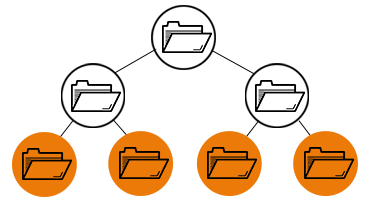
\includegraphics{Pictures/FileStorageHierarchy.png}
	\caption{File Storage: Aufbau des Hierarchiesystems, \citeauthor{redHat-storage}}
\end{figure}

File Storage wird häufig in Unternehmen und Organisationen eingesetzt, um gemeinsame Dateiserver bereitzustellen oder Daten in Cloud-Speicherdiensten wie Dropbox oder Google Drive zu speichern.
Auch wenn es von Betriebssystemen und Anwendungen gut unterstützt wird, kann die Performance und Skalierbarkeit von File Storage bei sehr großen Dateisystemen beeinträchtigt werden, was insbesondere bei stark frequentierten Anwendungen oder bei der Verarbeitung großer Datenmengen zum Problem werden kann. 

\begin{quote}
	Mit zunehmenden Datenvolumen erfordert das Skalieren von Dateispeichern das Hinzufügen neuer Hardwaregeräte oder den Austausch vorhandener Geräte durch solche mit höherer Kapazität. Dies kann im Laufe der Zeit teuer werden. \glqq As data volumes expand, scaling file storage requires [...]\grqq, (\cite{nx-fileScala}, Übersetzung des Autors)
\end{quote}

Laut Wahlmann (\citeyear{nx-fileScala}, Übersetzung des Autors) wird die Datenspeicherung bei zu vielen Daten nicht nur teuer, sondern auch unhandlich und zeitaufwändig. Der schnelle und einfache Zugriff auf jede einzelne Datei wird schwierig, wenn man zig Millionen von Dateien in Tausenden von Verzeichnissen auf Hunderten von Speichergrößen speichert. 

\newpage

\subsection{Block Storage}

Block Storage, auch genannt als Block-level Storage speichert Dateien auf SAN(Storage Area Networks) basierten Netzwerken oder auf Cloud-basierten Speicherumgebungen. Das System teilt Daten in Blöcke auf und speichert die separaten Teile jeweils mit einer eindeutigen Kennung, vgl. \cite{ibm-topics}.\\

Daten werden in Blöcken auf dem Datenträger gespeichert, die unabhängig voneinander adressiert werden können. Jeder Block ist eine feste Größe, typischerweise im Bereich von einigen Kilobytes bis hin zu einigen Megabytes. Diese Blöcke können im System an jeder Stelle gespeichert werden.

\begin{quote}
	Wenn auf Block Storage gespeicherte Daten abgerufen werden, verwendet das Server-Betriebssystem die eindeutige Adresse, um die Blöcke wieder zusammenzufügen und so die Datei zu erstellen. Der Vorteil besteht darin, dass das System nicht durch Verzeichnisse und Dateihierarchien navigieren muss, um auf die Datenblöcke zuzugreifen. Dadurch werden Effizienzen erzielt, da der Abruf von Daten schneller erfolgen kann, vgl. \cite{ibm-storage}.
\end{quote}

Typische Anwendungsbereiche des Block Storage sind Datenbanken, Virtualisierungsumgebungen und Anwendungen für Big Data-Analysen. Speicherung von strukturierten Daten wie Datenbanken, Virtuelle Maschinen und Betriebssysteme eignen sich besonders bei der Verwendung von Block Storage. Diese Art von Daten erfordert schnellen und direkten Zugriff auf bestimmte Bereiche des Speichers und muss häufig in Echtzeit ausgeführt werden. Block Storage eignet sich daher am besten für Anwendungen mit hohen Anforderungen an die Leistung und niedriger Latenzzeit.

\newpage

\subsection{Object Storage}

Object Storage hat sich als Speichertechnologie in den letzten Jahren immer stärker etabliert und wird von vielen Unternehmen als Alternative zu traditionellen Speicherlösungen wie Block- oder File Storage angesehen. Die ersten Object Storage Systeme wurden bereits in den 1990er Jahren entwickelt, aber erst mit dem Aufkommen von Big Data, IoT und der Cloud-Nutzung 
 hat es einen breiteren Einsatz gefunden. Heute bieten viele Cloud Provider wie Amazon Web Services (AWS) und Google Cloud Platform (GCP) Object Storage als einen ihrer Haupt-Cloud-Services an.
 
\begin{quote}
	Object Storage ist für den Umgang mit großen Datenvolumen und unstrukturierten Daten entwickelt wurden. Sie speichert Daten als eigenständige Objekte, die aus Daten und Metadaten bestehen und einen eindeutigen Identifier (UID) haben (\glqq Object storage (aka object-based storage) is a type of data storage used to [...]\grqq, \cite{dataCore-OS}, Übersetzung des Autors).
\end{quote}

Im Gegensatz zu hierarchischen Systemen wie beim File Storage ist das Speichersystem flach strukturiert. Durch die einfache API Anbindung kann es mit vorhandenen Anwendungen integriert werden. Nutzer können detaillierte Informationen wie beispielsweise Erstellerangaben, Schlüsselwörter sowie Sicherheit-und Datenschutzrichtlinien hinterlegen. Diese Daten bezeichnet man als Metadaten.\\

Laut \citeauthor{nx-fileScala}, 2022 ist Skalierbarkeit der Hauptvorteil, da bei der Speicherung von Petabyte und Exabyte alle Objekte in einem Namespace abgelegt werden. Selbst wenn dieser Namespace auf Hunderte von Hardwaregeräten und Standorten verteilt ist, können alle Objekte schnell abgerufen werden. Andere Vorteile von Objekt Storage beinhalten die Datenintegritätsprüfung, im Englischen bekannt als \glqq erasure coding\grqq und die Datenanalyse.\\

Auch Object Storage hat seine Nachteile. Laut \citeauthor{redHat-storage} muss das Objekt nach der Speicherung bei Veränderung komplett neu überschrieben werden. Sie sind für traditionelle Datenbanken nicht geeignet, da das Schreiben von Objekten Zeit beansprucht und man sich mit der API auseinandersetzen muss, vgl. \citeauthor{redHat-storage}.\\

Insgesamt bietet Object Storage eine skalierbare und flexible Methode zur Speicherung von unstrukturierten Daten. Organisationen sollten jedoch die Vor- und Nachteile von Object Storage im Kontext ihrer spezifischen Anwendungsfälle abwägen, um eine fundierte Entscheidung über die beste Speichermethode zu treffen.\\

%TODO Object Storage Entscheidung

Da leoticket Daten wie Rechnungen und Tickets als Dateien speichern und abrufen abruft, ist Object Storage die richtige Speicherart. 

Für leoticket ist die Object Storage Variante die am Besten geeignetste Speicherlösung, da ... %TODO Satz weiterschreiben

\newpage

\section{Aktuelle Speichertechnologien im Markt}

Die beiden größten Cloud-Speicheranbieter, Amazon Web Services (AWS) und Google Cloud Platform (GCP), bieten eine Vielzahl von Speicherlösungen an, die auf die Bedürfnisse von Unternehmen zugeschnitten sind.\\ 

In diesem Kapitel werden die aktuellen Speichertechnologien auf dem Markt untersucht, wobei der Fokus auf den Angeboten von AWS und GCP liegt. Um eine Vergleichsgrundlage zwischen AWS und GCP zu schaffen, werden die verschiedenen Aspekte wie sichere Speicherung, Hochverfügbarkeit, Leistung, Kosten, API Anbindung und die Bereitstellung der Dateien betrachtet. Dieses Vorgehen dient dazu, zu ermitteln, welche Speicherart sich am besten für welche Anforderungen eignet. Als Kontrast dazu wird das Open-Source-Objektspeichersystem MinIO betrachtet.\\

AWS bietet eine Reihe von Speicheroptionen an, darunter Amazon S3 (Simple Storage Service). Amazon S3 ist ein Object Storage-Service, der für die Speicherung und den schnellen Abruf von unstrukturierten Daten wie Videos, Fotos und Dokumenten ausgelegt ist.

Google Cloud Platform bietet ebenfalls eine Vielzahl von Speicherlösungen an, darunter Google Cloud Storage. Google Cloud Storage ist ein Object Storage-Service, der für die Speicherung von unstrukturierten Daten wie Bildern, Videos und Dokumenten ausgelegt ist.\\
 
Insgesamt bieten AWS und Google Cloud Platform eine Vielzahl von Speicherlösungen an, die auf die Bedürfnisse von Unternehmen zugeschnitten sind. Organisationen sollten jedoch die Vor- und Nachteile jeder Speicherlösung abwägen, um die beste Lösung für ihre spezifischen Anforderungen zu finden.

\newpage

\subsection{Eigenschaften}

Im vorliegenden Abschnitt werden Amazon S3 und Google Cloud Storage in Bezug auf verschiedene Kriterien untersucht. Dabei werden zunächst die Eigenschaften von AWS S3 erläutert, gefolgt von einer Betrachtung von GC Storage. Ziel ist es, die Unterschiede zwischen den beiden Anbietern hervorzuheben und eine Entscheidungshilfe zu bieten, welche Plattform für die Anforderungen von \glqq leoticket\grqq am besten geeignet ist. Die Auswahl der Kriterien erfolgt in Anlehnung an die spezifischen Anforderungen von \glqq leoticket\grqq.

%TODO Aws und GCP Definition?

\newpage

\subsubsection{Sichere Speicherung}

Viele Anbieter von Object Storage-Lösungen bieten integrierte Verschlüsselungsmöglichkeiten an, um sicherzustellen, dass Daten sowohl in Ruhe als auch in Bewegung geschützt sind. Dabei können unterschiedliche Verschlüsselungsmethoden zum Einsatz kommen. In Bezug auf die sichere Speicherung bieten sowohl AWS als auch GCP verschiedene Optionen für die Verschlüsselung von Daten.Die Sicherheit der gespeicherten Daten ist von entscheidender Bedeutung, um die Integrität und Vertraulichkeit der Daten zu gewährleisten.\\

\textbf{Amazon S3}\\

In diesem Unterabschnitt werden die verschiedenen Sicherheitsfunktionen von Amazon S3 untersucht.\\

IAM (Identity and Access Management) ist ein wichtiger Bestandteil von AWS und ermöglicht es Benutzern, Gruppen und Rollen zu erstellen, um den Zugriff auf S3 zu verwalten. Benutzer können individuelle Berechtigungen zugewiesen werden, während Gruppen und Rollen mehrere Benutzer mit denselben Berechtigungen zusammenfassen können. Auf S3-Buckets und Objekte kann man eine granuläre Zugriffssteuerung anwenden. Benutzer, Gruppen oder Rollen können so berechtigt werden, den Zugriff auf bestimmte Buckets und Objekte zu beschränken oder zu erlauben. "Beim Erteilen von Berechtigungen in Amazon S3 entscheiden Sie [...]."\cite{aws-iam-s3}\\

Eine weitere wichtige Sicherheitsfunktion von Amazon S3 ist die Datenverschlüsselung. S3 bietet eine Vielzahl von Verschlüsselungsoptionen für die serverseitige und clientseitige Verschlüsselung. Da für leoticket die clientseitige Verschlüsselung nicht in Frage kommt, liegt der Fokus auf der serverseitigen Verschlüsselung. Es gibt drei Methoden, darunter die serverseitige Verschlüsselung mit Amazon S3-verwalteten Schlüsseln (SSE-S3), mit KMS-verwalteten Schlüsseln (SSE-KMS) und die SSE-C. Diese Optionen ermöglichen es Benutzern, die Verschlüsselung auf ihre spezifischen Anforderungen abzustimmen und so die Sicherheit der Daten zu gewährleisten.

Laut \citeauthor{aws-iam-s3} nutzen Buckets standardmäßig die SSE-S3 Methode. Für die Verschlüsselung wird die 256-bit Advanced Encryption Standard (AES-256) verwendet. Seit dem 5. Januar 2023 sind alle neu erstellen Buckets auf SSE-S3 ausgelegt. Alle neuen Objekte sind beim Hochladen automatisch verschlüsselt, ohne weitere Zusatzkosten und keine Einbußung der Leistung.

\begin{quote}
	Die Serverseitige Verschlüsselung schützt die Daten at rest. Amazon S3 verschlüsselt jedes Objekt mit einem eindeutigen Schlüssel. Als zusätzliche Sicherheitsmaßnahme werden diese eindeutigen Schlüssel mit einem weiteren Schlüssel verschlüsselt, welches in regelmäßigen Abständen rotiert wird, vgl. \cite{aws-iam-s3}
\end{quote}

Amazon S3 stellt auch die SSE-KMS als Auswahl zur Verfügung. AWS-KMS ist ein Dienst, dass einen Schlüsselverwaltungssystem zur Verfügung stellt. Es verschlüsselt die Objekt Daten und speichert die S3 Checksum, das im Objekt Metadaten steckt, in verschlüsselter Form. Man kann die SSE-KMS in der AWS Management Konsole oder über die AWS KMS API verwalten. Jedoch gibt es zusätzliche Kosten bei der Verwendung der Methode. Dazu mehr im Kosten Abschnitt. Bei der Nutzung von AWS-SSE gibt es zwei Methoden. Einmal die AWS managed key oder die customer managed key. Es unterstützt die \glqq envelope encryption\grqq. Das bedeutet, das die Schlüssel für die Daten durch einen Master Key verschlüsselt wird. Dies erleichtert die Verwaltung der Schlüssel.\\

Bei der AWS managed key Variante wird automatisch ein Schlüssel erstellt, sobald ein Objekt in ein Bucket hochgeladen wird. Dieser generierte Schlüssel wird dann für die Ver- und Entschlüsselung der Daten verwendet. Wenn man einen eigenen Schlüssel bei KMS verwenden möchte, dann erstellt man zuerst einen symmetrischen Key vor der KMS Konfiguration. Bei der Bucket Erstellung kann man anschließend den selbst-erstellten Key angeben. Die Nutzung von Customer Managed Keys hat einige Vorteile, die den Anforderungen von leoticket entspricht. Selbsterstellte Schlüssel bieten mehr Flexibilität und Kontrolle. Man kann sie selber erstellen, rotieren und deaktivieren. Hinzufügend kann man auch Zugriffskontrollen und Auditierung für den Schutz der Daten konfigurieren.\\

Wenn man die SSE-KMS Variante aussucht, kann man auch die S3 Bucket Key Funktion aktivieren. Dies kann die Request Kosten bis zu 99 Prozent reduzieren, indem die Request Traffic von Amazon S3 zu AWS KMS reduziert wird. Durch die Aktivierung der S3 Bucket Key für einen Bucket werden unique data keys für die Objekte im Bucket erstellt. Diese Bucket Keys werden für eine bestimmte Zeit verwendet, welches Abrufe zu Amazon S3 nach AWS KMS reduziert um Verschlüsselungsoperationen durchzuführen.\\

Zuletzt gibt es noch die SSE-C (server-side encryption with customer-provided keys). Bei der SSE-C stellt der Customer seinen eigenen Schlüssel zur Verfügung. Dieser Schlüssel wird nicht von Amazon S3 gespeichert, im Gegensatz bei AWS KMS. Amazon S3 übernimmt mit dem bereitgestellten Schlüssel die Datenverschlüsselung beim Schreiben sowie die Datenentschlüsselung beim Zugriff auf Objekte. Amazon S3 entfernt anschließend den Schlüssel aus dem Speicher. Da Amazon S3 den Schlüssel nicht speichert, sepeichert er den zufällig generierten HMAC (Hash-baded Message Authentication Code) Wert vom Encryption Key um zukünftige Requests zu validieren."Note: Amazon S3 does not store the encryption key that you provide. [...]", \cite{aws-sse-c}.\\

Object Ownership ist eine weitere wichtige Sicherheitsfunktion von Amazon S3. Mit Object Ownership können Benutzer oder Gruppen die Eigentümerschaft von Objekten in S3-Buckets besitzen. Dies bedeutet, dass nur autorisierte Benutzer die Berechtigung haben, Objekte zu löschen oder zu ändern, was die Sicherheit der Daten erhöht.\glqq S3 Object Ownership ist eine Einstellung auf Amazon-S3-Bucket-Ebene, mit der Sie Zugriffskontrolllisten (ACLs) deaktivieren und das Eigentum an jedem Objekt in Ihrem Bucket übernehmen können, [...]." \cite{aws-iam-s3}\\ 

\newpage

AWS empfiehlt die ACL (Access Control List) auf Bucket-Ebenen deaktiviert zu lassen. Alle Objekte eines Buckets gehört so dem Bucket Owner. Laut \citeauthor{aws-iam-s3} verfügt Object Ownership über drei Einstellungen, mit denen man die Eigentümerschaft von Objekten steuern kann.

\begin{figure}[h]
\centering
	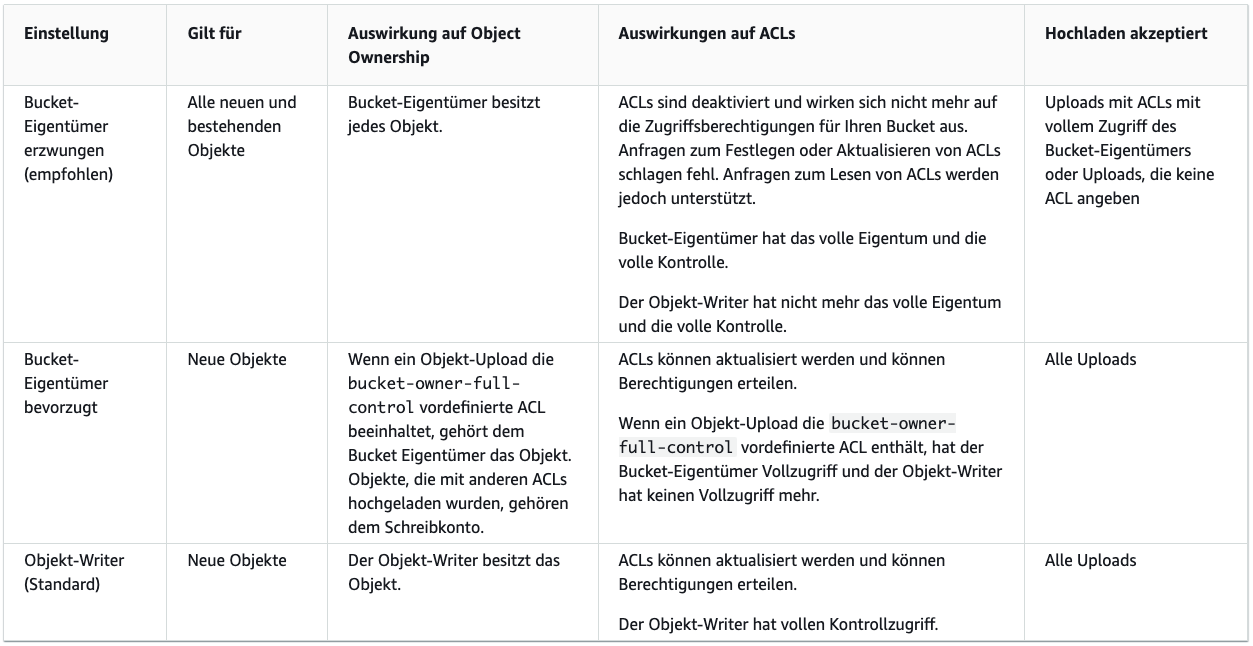
\includegraphics[width=13cm,keepaspectratio]{Pictures/objectOwnershipTable.png}
	\caption{Einstellungen für Object Ownership, \citeurl{aws-iam-s3}}
\end{figure}

Laut \citeauthor{aws-iam-s3} zeigt die obige Tabelle die Auswirkungen, die jede Einstellung für Object Ownership auf ACLs, Objekte, Objekteigentümer und Objekt-Uploads hat.\\

Logging ist ein weiterer Aspekt der Amazon S3-Sicherheit. S3 bietet verschiedene Logging-Optionen, darunter Bucket Logging und Object-Level Logging, die es Benutzern ermöglichen, Zugriffe auf S3-Objekte aufzuzeichnen und zu überwachen. Diese Funktionen sind entscheidend, um Compliance-Anforderungen zu erfüllen und verdächtige Aktivitäten zu erkennen. AWS bietet eine Vielzahl von tools zur Überwachung der Amazon S3 Ressourcen. Darunter die Amazon CloudWatch Alarms, AWS CloudTrail Logs, Amazon S3 Access Logs und die AWS Trusted Advisor.\\

%TODO compliance

\newpage

\textbf{Google Cloud Storage}\\

Auch Google Cloud bietet eine Vielzahl an Sicherheitsfunktionen, um sicherzustellen, dass Daten in der Cloud sicher gespeichert und geschützt sind. Unter anderem die Datenverschlüsselung. Google Cloud bietet genau wie Amazon S3 Serverseitige Verschlüsselung an. Hier unterscheidet man zwischen Google-managed Keys, Customer-managed encryption keys und die Customer-supplied encryption keys. Google-managed encryption ist die Standard Verschlüsselungsoption von Google Cloud. Cloud Storage verschlüsselt die Daten serverseitig, bevor die Daten auf die Festplatte geschrieben werden. 

\begin{quote}
	Die Standard Variante verwaltet für den Nutzer die Encryption Keys in ihrem eigenen Key Management System. Auch Google verwendet für die Verschlüsselung die AES-256 wie AWS. Als Nutzer muss man bei dieser Varianet keine Einstellungen berücksichtigen. Daten werden automatisch verschlüsselt beim Abruf, vgl. \cite{gcp-encrypt}.
\end{quote}

Wenn man mehr Kontrolle über die Schlüssel haben möchte, dann gibt es die Customer-managed encryption Option. Die Schlüssel werden von Cloud KMS (Cloud Key Management Service) erstellt und verwaltet. Diese Schlüssel werden vom Nutzer anschließend extern oder in einem HSM Cluster gespeichert. Customer Keys kann man für indivduelle Objekte benutzen oder einen Bucket so einstellen, dass er einen Standard Key für alle neuen Objekte verwendet. Der erstellte Schlüssel wird für die Verschlüsselung der Objektdaten, die CRC32C Checksum des Objekts und für die MD5 Hash verwendet. Als zusätzlichen Schutz gibt es die Service Agents, auch genannt als service accounts. Diesem Agent kann man bestimmte Rechte geben, sodass es Zugriff auf den gewünschten Encryption Key hat, um damit Objekte verschlüsseln zu können.\\

Zuletzt gibt es noch die Customer-supplied encryption keys. Als zusätzliche Sicherheitsebene zu Google-managed encryption keys können Nutzer ihren eigenen AES-256 Encryption Key bereitstellen, welches als Base64 encoded ist. Bei dieser Variante wird der Schlüssel nicht von Google Cloud gespeichert oder verwaltet. Die Nutzer müssen diese Schlüssel selber verwalten und speichern. Um zukünftige Requests zu validieren speichert Google Cloud einen kryptografischen Hash vom Schlüssel. Jedoch kann der Encryption Key nicht aus dem Hash regeneriert werden oder den Hash nicht zum Entschlüsseln anwenden.\\

Des weiteren gibt es auch in Google Cloud Zugriffskontrolleinstellungen, mit der Nutzer genau steuern können, wer auf ihre Daten zugreifen kann. Den Zugriff kann man auf Bucket- und Objektebene steuern und Benutzern und Gruppen bestimmte Rollen zuweisen. Dabei wird zwischen Uniform und Fine-grained unterschieden. Uniform Access Control (UAC) ermöglicht es, den Zugriff auf einen gesamten Bucket in Google Cloud Storage auf der Ebene von Rollen zuzuweisen. Dazu können verschiedene vordefinierte Rollen wie "Leser", "Schreiber" oder "Besitzer" verwendet werden, die festlegen, welche Aktionen ein Benutzer auf dem Bucket ausführen darf. UAC ist eine einfachere Methode zur Zugriffskontrolle, da die Zugriffsrechte auf Bucket-Ebene vergeben werden. Das bedeutet, dass alle Objekte in dem Bucket automatisch dieselben Zugriffsrechte haben.\\

Fine-Grained Access Control (FGAC) hingegen ermöglicht es, die Zugriffskontrolle auf die Ebene von Objekten oder sogar auf Teile von Objekten herunterzubrechen. Das bedeutet, dass jeder Benutzer oder jede Gruppe individuelle Zugriffsrechte auf bestimmte Objekte oder Teile von Objekten haben kann. Mit FGAC kann man sehr granulare Zugriffssteuerungen implementieren. Es ist eine mächtige Methode, aber auch komplexer und zeitaufwändiger zu implementieren als UAC. Mit Cloud IAM können auch rollenbasierte Zugriffssteuerungen für Bucket- unObjektebene ähnlich wie bei AWS umgesetzt werden.\\

Weitere Funktionen die Google Cloud anbietet ist Objekt Versioning, Audit Logging, Bucket Locks, VPC Service Controls, Data Loss Prevention und Identity-Aware Proxy.

\newpage

\subsubsection{Hochverfügbarkeit}

\textbf{Amazon S3}\\

Amazon S3 ist ein skalierbarer und hochverfügbarer Objekt Storage, der eine Verfügbarkeit von 99.99 Prozent garantiert.\glqq Designed to provide 99.999999999 percent durability and 99.99 percent availability of objects over a given year.\grqq, \cite{aws-availability}\\

Dies wird durch die Verwendung von Multi-Availability Zone Architekturen erreicht, die eine automatische Replikation von Daten in verschiedenen physischen Standorten ermöglichen. Die Multi-Availability Zone Architektur von Amazon S3 basiert auf der Aufteilung von Daten in mehrere geografisch getrennte Verfügbarkeitszonen (AZs). Jede AZ besteht aus mehreren physischen Rechenzentren, die sich in einem geografisch getrennten Gebiet befinden. Jede AZ ist vollständig unabhängig und bietet eine hohe Redundanz und Verfügbarkeit. Wenn ein Benutzer ein Objekt in Amazon S3 hochlädt, wird es automatisch in mehrere AZs repliziert.um sicherzustellen, dass das Objekt auch bei AUsfällen in einer AZ weiterhin verfügbar ist. Im Falle eines Ausfalls einer AZ wird Amazon S3 automatisch die Anfragen auf eine andere AZ umleiten, um eine ununterbrochene Verfügbarkeit des Objekts sicherzustellen. Durch die Cross-Region Replikation werden Daten automatisch in andere AWS-Regionen repliziert. Dadurch kann eine hohe Verfügbarkeit der Daten im Falle eines Ausfalls einer gesamten AWS-Region gewährleistet werden.\\

Amazon S3 bietet auch eine hohe Verfügbarkeit von Metadaten, die für den Zugriff auf Objekte verwendet werden. Metadaten werden automatisch in mehrere AZs repliziert, um sicherzustellen, dass die Metadaten auch im Falle eines Ausfalls einer AZ verfügbar bleiben. Zusätzlich zu Multi-Availability Zone Architekturen verwendet Amazon S3 auch Fehlerkorrektur- und Erkennungsmechanismen wie CRC-Prüfungen, um die Integrität von Daten sicherzustellen und sicherzustellen, dass die gespeicherten Daten stets korrekt sind.\\

Durch Aktivierung der Versionierung wird jeder Objektversion, die in einem Amazon S-Bucket gespeichert ist, eine eindeutige Versions-ID zugewiesen. Wenn eine Objektversion versehentlich gelöscht oder überschrieben wird, kann die vorherige Version wiederhergestellt werden.\\

Um eine hohe Verfügbarkeit bereitzustellen, stell Amazon S3 außerdem noch die S3-Transfer Acceleration zur Verfügung. Durch die Verwendung von Amazon S3-Transfer Acceleration können Benutzer die Übertragung großer Datenmengen beschleunigen, indem ein optimierter Netzwerkpfad genutzt wird. Dadurch kann de Verfügbarkeit der Daten verbessert werden, indem Verbindungsprobleme minimiert werden.\\

Um die Leistung von Amazon S3 zu überwachen und auf mögliche Probleme reagieren zu können wird CloudWatch bereitgestellt. Dadurch können Ausfallzeiten minimiert werden und herausfinden, an welchen Momenten die Verfügbarkeit am geringsten ist.

Insgesamt bietet Amazon S3 eine hochverfügbare und zuverlässige Speicherlösung, die durch Multi-Availability Zone Architekturen und Fehlerkorrekturmechanismen eine Verfügbarkeit von 99,99 Prozent gewährleistet.

\newpage

\textbf{Google Cloud Storage}\\

Laut \cite{gcp-sla} wird die Verfügbarkeit von Google Cloud Storage als Service Level Agreement (SLA) angegeben, das die garantierte Verfügbarkeit für den Dienst definiert. Gemäß dem aktuellen SLA von Google Cloud Storage beträgt die garantierte Verfügbarkeit für Multi-Regionaler Speicher 99,95 Prozent und für Regionale Speicher 99,9 Prozent. Diese Zahlen geben an, dass Google Cloud Storage darauf ausgelegt ist, eine sehr hohe Verfügbarkeit zu gewährleisten. In der folgenden Tabelle werden diese Werte nochmals belegt.

\begin{figure}[h]
	\centering
	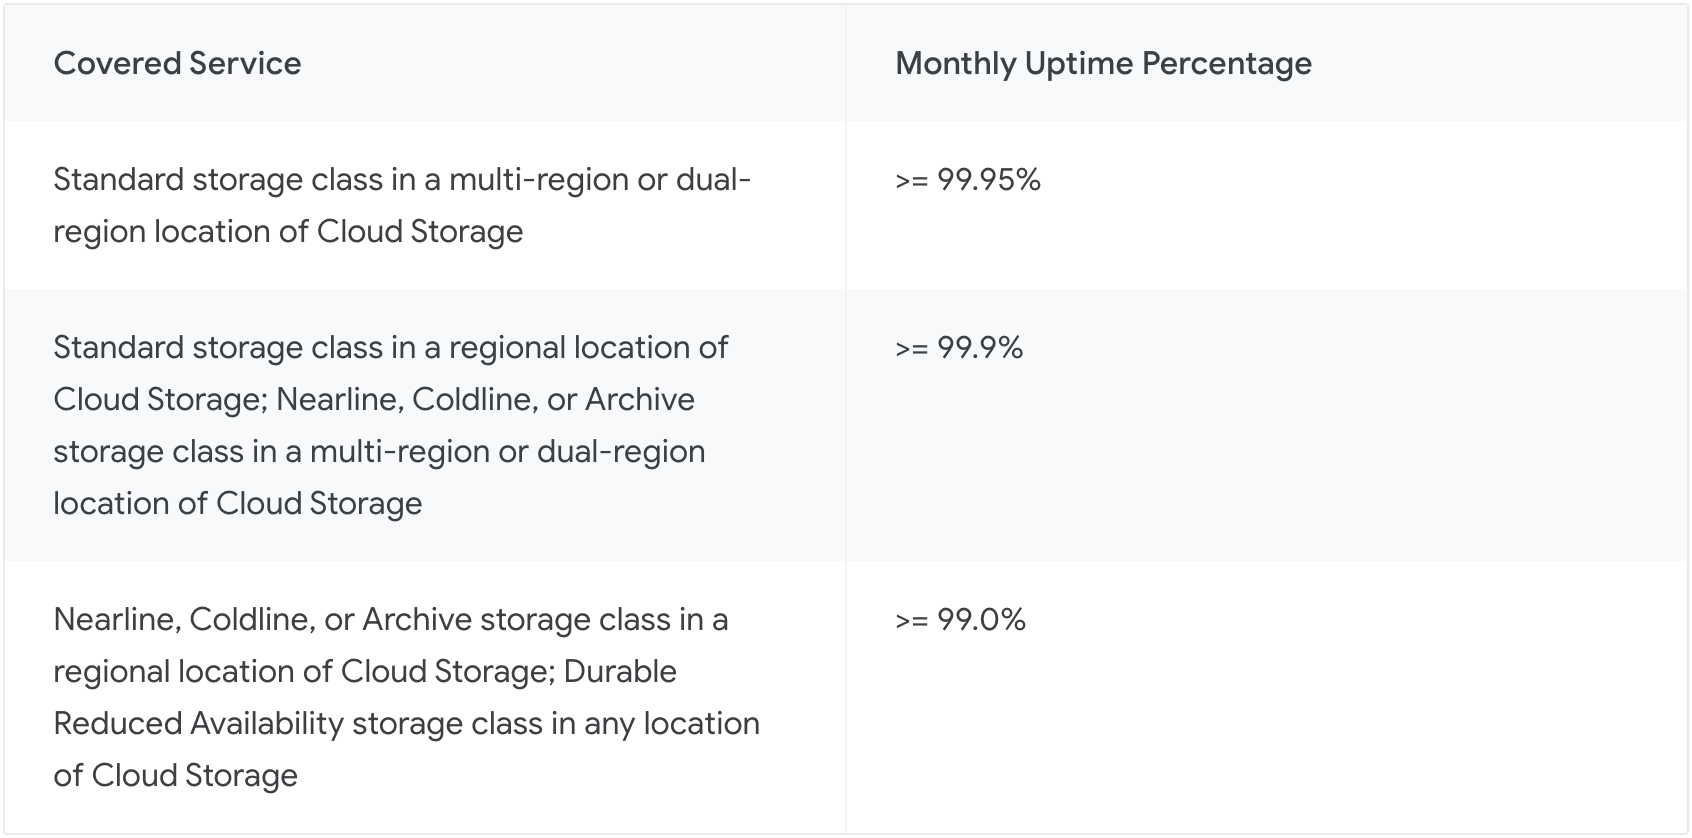
\includegraphics[width=12cm,keepaspectratio]{Pictures/GCSLA.png}
	\caption{Verfügbarkeit der Speicherklassen gemäß Google Cloud Storage SLA \citeurl{gcp-sla} }
\end{figure}

Es ist jedoch zu beachten, dass die tatsächliche Verfügbarkeit von Google Cloud Storage von mehreren Faktoren abhängt, einschließlich der spezifischen Konfiguration, dem Datenzugriffsmuster, der Netzwerkverfügbarkeit und anderen betrieblichen Variablen. Es ist daher möglich, dass die tatsächliche Verfügbarkeit in der Praxis leicht von der garantierten Verfügbarkeit abweicht.

Auch Google Cloud Storage bietet die Multi-Region Storage an. Dies ermöglicht die Speicherung von Daten in mehreren Regionen weltweit. Dadurch werden die Daten redundant repliziert und bleiben auch im Falle eines Ausfalls einer Region verfügbar.\\ 

Object Versioning bietet wie AWS die Möglichkeit Objektversionen beizubehalten. Dadurch können vorherige Versionen von Objekten wiederhergestellt werden, falls sie versehentlich gelöscht oder überschrieben werden.\\

Mit der Bucket- und Objekt Replikation können Daten automatisch in andere Regionen oder Projekte repliziert werden. Dies ermöglicht eine geografische Redundanz und verbessert die Verfügbarkeit der Daten. Google Cloud Storage verwendet verteilte Speichersysteme eine redundante Infrastruktur, um eine hohe Datensicherheit- und Verfügbarkeit zu gewährleisten. Die Daten werden in mehreren Datenzentren repliziert, um Ausfälle zu vermeiden.\\

Ein weiterer Punkt ist die Monitoring und Fehlererkennung wie Stackdriver Monitoring, um die Leistung und Verfügbarkeit von google Cloud Storage zu überwachen und auf potenzielle Probleme zu reagieren.

\newpage

\subsubsection{Kosten}

In diesem Abschnitt werden die Kosten von Amazon S3 und Google Cloud Storage betrachtet. Dabei werden die allgemeinen Kosten erläutert für welche die Cloud Provider Gebühren fordern. Bei der Kostenanalyse werden anschließend die Daten von leoticket genommen und eine grobe Abschätzung der Kosten durchgeführt.\\

Amazon S3 setzt Gebühren für die Speicherung, Anforderungen und Datenabrufe, Datenübertragung, Verwaltung und Analyse, Replikation und S3 Objekt Lambda. Für die Speicherung ist die Gebühr abhängig von der Größe der Objekte, der Speicherdauer während des Monats und der Speicherklasse. Es gibt verschiedene Speicherklassen zur Auswahl, die für verschiedenen Use Cases geeignet sind. Das wären die S3 Standard, S3 Intelligent-Tiering, S3 Standard – Infrequent Access, S3 One Zone – Infrequent Access, S3 Glacier Instant Retrieval, S3 Glacier Flexible Retrieval (früher S3 Glacier) und S3 Glacier Deep Archive. S3 Glacier wird in dieser Arbeit nicht behandelt, da leoticket keine Anwendung für diese Speicherklasse hat. Es werden die Speicherklassen S3 Standard, S3 Intelligent-Tiering, S3 Standard - Infrequent Access und S3 One Zone - Infrequent Access untersucht.

Um das Ganze zu veranschaulichen, werden die Preise durch die untere Tabelle präsentiert.

\begin{figure}[h]
	\centering
	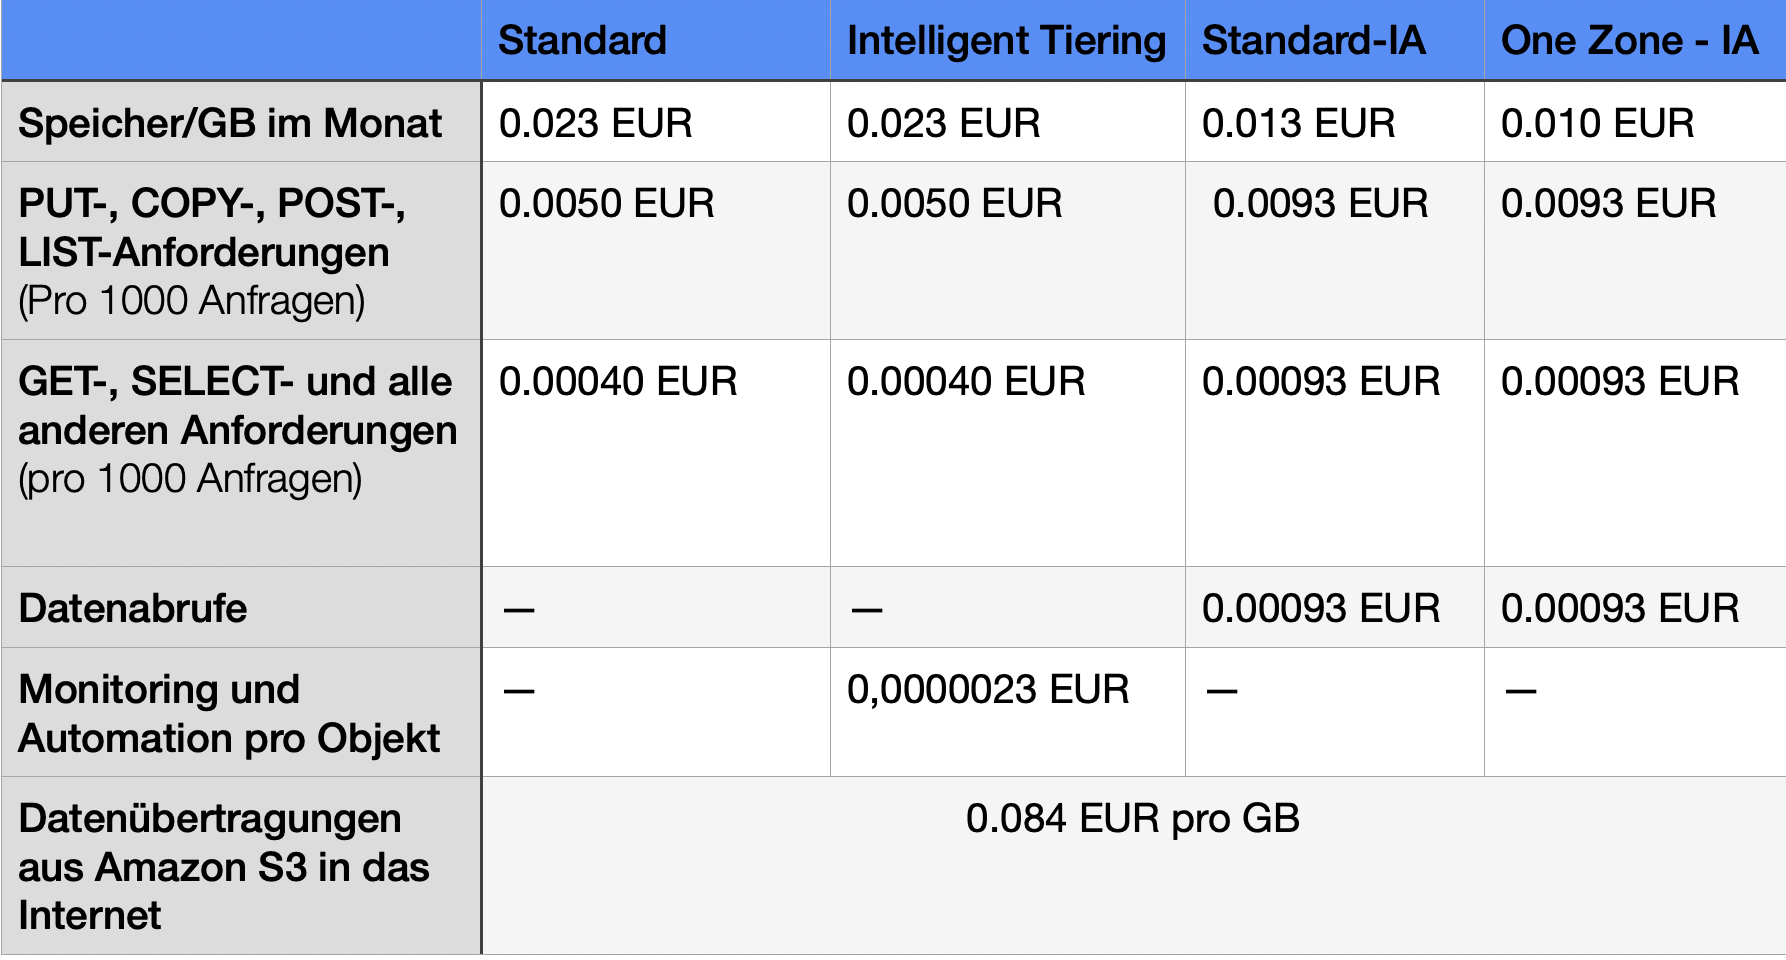
\includegraphics[width=12cm,keepaspectratio]{Pictures/AllgKostenAWS.png}
	\caption{Übersicht der Kosten der AWS S3 Speicherklassen}
\end{figure}

In der obigen Tabelle werden die Standard Preise von den verschiedenen Speicherklassen von Amazon S3 dargestellt. Die One Zone -IA hat dabei die niedrigsten kosten im Vergleich zur Standard Speicherklasse. Jedoch sind die Kosten für die Anfragen beim One zone - IA genauso wie beim Standard - IA höher als beim Standard und Intelligent Tiering. Zusätzlich werden bei Datenabrufen in den Fällen von Standard-IA und One Zone-IA Gebühren von 0.01 USD pro GB erhoben. So sind die Speicherklassen Standard und Intelligent Tiering für häufig abgerufene Daten, bei denen eine sofortige Verfügbarkeit und eine niedrige Latenzzeit erforderlich ist geeignet. Standard bietet eine hohe Leistung und ist ideal für Anwendungen, bei denen schneller Zugriff auf die Daten erforderlich ist. Die Intelligent Tiering eignet sich für Daten mit wechselndem Zugriffsverhalten. Sie analysiert das Zugriffsmuster der Objekte und verschiebt sie automatisch zwischen zwei Zugriffstiers. Dadurch kann man Kosten sparen, da man für den tatsächlichen Zugriff auf die Daten bezahlt und nicht für eine dauerhafte Speicherung in der teureren Speicherklassen.\\

Standard-IA und One Zone-IA bieten kostengünstigere Optionen für die Speicherung der Daten. Die Standard-IA ist für Daten geeignet, auf die weniger häufig zugegriffen wird, aber bei Bedarf schnell verfügbar sein müssen. Im Vergleich zur Standardklasse sind die Kosten für die Speicherung niedriger, aber es fallen zusätzliche Gebühren für den Datenabruf an. Wenn Daten von zwei Speicherklassen hergeschoben werden, dann fallen Kosten für den Speicherklassenwechsel an. Diese hängen von der Datenmenge ab, die verschoben werden.\\

Die One Zone-IA ist für Daten geeignet, auf die selten abgerufen werden, jedoch mit einer Einschränkung. Anders als bei den anderen Speicherklassen wird One Zone-IA nur in einem einzelnen Availability Zone in einer bestimmten Region gespeichert. Dies bedeutet, dass die Daten in einer einzigen AZ verfügbar sind und ein potenzieller Datenverlust auftreten kann, wenn diese AZ nicht verfügbar ist.\\

Bei der Replikation von Daten zahlt man gebühren für die Speicherung in den ausgewählten Ziel-S3-Speicherklassen, für die primäre Kopie, für Replikations-PUT Anforderungen und für anwendbare Gebühren für den Speicherabruf mit seltenem Zugriff. Laut aws preise zahlt man auch für den regionenübergreifenden Datentransfer OUT von S3 zu jeder Zielregion. Die Preise für Speicher- und PUT-Anfragen für die replizierte Kopie basieren auf den ausgewählten AWS-Zielregionen, während die Preise für Datenübertragungen zwischen den Regionen auf der AWS-Quellregion basieren. Wenn man S3 Replication Time Control nutzt, zahlt man eine Datenübertragungsgebühr für die Replikationszeitsteuerung sowie die Gebühren für S3-Replikationsmetriken, die zum selben Tarif abgerechnet werden wie angepasste Amazon-CloudWatch-Metriken. Die kosten für die S3 Replication Time Control-Datenübertragung beträgt pro GB 0.015 USD. https://aws.amazon.com/de/s3/pricing/ \\


Auch bei der Objekt Versionierung fallen Kosten an, wenn man ältere Versionen von Objekten beibehalten möchte. Die Kosten beziehen sich auf den zusätzlichen Speicherplatz, der für die Aufbewahrung der Versionen verwendet wird. Für das Tagging von benutzerdefinierten Metadaten bei Objekten selbst fallen keine direkten Kosten an. Allerdings können Kosten für das Abrufen von Tags über die S3-API(z.B. mit der ListObjects- oder GetObject-Operationen) anfallen, da dies als Datenabruf betrachtet wird und entsprechende Gebühren gemäß den AWS-Preisen Datenzugriff erhoben werden. Es ist zu beachten, dass die genauen Preise für Objektversionierung und Tagging von Amazon S3 sich im Laufe der Zeit ändern können.\\

Die genauen Preise und Kostendetails für S3 Standard IA können sich im Laufe der Zeit ändern. Es wird empfohlen, die aktuellsten Informationen auf der offiziellen AWS-Preisseite oder im AWS-Kostenrechner zu überprüfen, um eine genaue Kosteneinschätzung zu erhalten.

\newpage

\textbf{Google Cloud Storage}\\

Google Cloud Storage setzt Preise für die Komponenten Datenspeicher, Datenverarbeitung und Netzwerknutzung. Beim Datenspeicher ist wie bei Amazon S3 die Menge der in den Buckets gespeicherten Daten bedeutend. Preise für Speicher hängen von der Speicherklasse der Daten und dem Standort der Buckets ab. Bei der Datenverarbeitung werden Gebühren für die von Cloud Storage durchgeführten Verarbeitung, einschließlich Vorgangsgebühren, anwendbarer Abrufgebühren und Replikation zwischen Regionen erhoben. Bei der Netzwerknutzung werden Gebühren für die Menge der aus den Buckets gelesenen oder zwischen diesen verschobenen Daten erhoben. Google Cloud Storage bietet vier Speicherklassen an von denen drei untersucht werden. Die Standard, Nearline und Coldline. Diese drei Speicherklassen haben unterschiedliche Leistungseigenschaften und Kosten. Die Preise variieren je nach gewählter Speicherklasse.\\

Um den Vergleich zwischen Amazon S3 und Google Cloud Storage zu veranschaulichen wird eine Tabelle in der unteren Abbildung gezeigt.(siehe Abb. 2.2.3)

\begin{figure}[h]
	\centering
	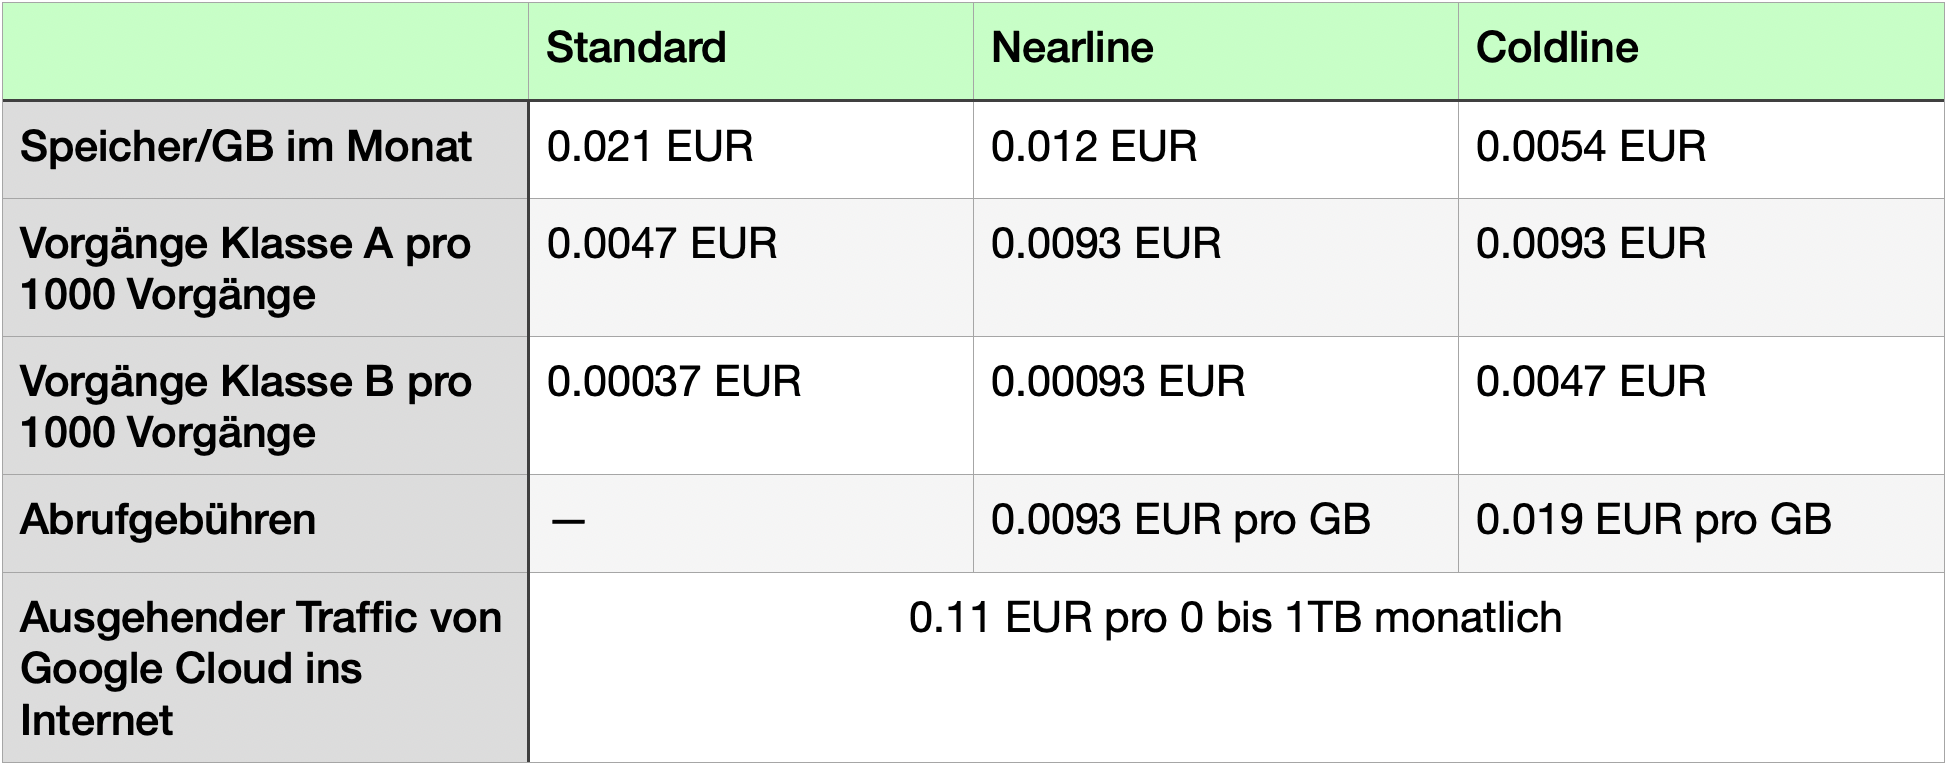
\includegraphics[width=12cm,keepaspectratio]{Pictures/GCStorageClassKosten.png}
	\caption{Vergleich der Kosten von Google Cloud Storage Speicherklassen}
\end{figure}

Ähnlich wie bei Amazon S3 sind die Speicherkosten der Nearline und Coldline geringer als die Standard Speicherklasse. Dafür werden Gebühren für die Datenabrufe bei Nearline und Coldline erhoben. Die verschiedenen Speicherklassen sind für unterschiedliche Anwendungsfälle ähnlich wie bei Amazon S3 konzipiert. Die Standard Storage-Klasse bietet hohe Performance, niedrige Latenzzeiten und hohe Verfügbarkeit. Sie eignet sich gut für häufig genutzte Daten, bei denen schneller Zugriff und gerine Latenz von Bedeutung sind. Beispiele dafür sind aktive Anwendungen, Datenbanken oder Inhalte mit hohem Durchsatz. Die Nearline Storage-Klasse ist für seltener genutzte Daten konzipiert, auf die jedoch mit niedriger Latenzzeit zugegriffen werden muss. Es bietet niedrigere Speicherkosten als die Standard Storage, jedoch mit einer etwas längeren Zugriffszeit. Es eignet sich für Backup-Daten, Archivierung und lange Speicherung. Letztere Speicherklasse, die Coldline Storage ist für Daten ausgelegt, auf die selten zugegriffen wird und bei denen eine längere Zugriffszeit akzeptabel ist. Es bietet die niedrigsten Speicherkosten an. Sie eignet sich gut für langfristige Archivierung, Compliance-Daten und Backup-Daten.\\ 

Zusätzliche Kosten, die nicht in der Tabelle aufgelistet sind, sind die Kosten für die Replikation der Daten. Auf Wunsch können Nutzer in Cloud Storage Daten innerhalb einer Region, in Dual-Regionen oder Multiregionen replizieren. Zusätzlich zu den Daten, die in den hochgeladenen Objekten enthalten sind, werden benutzerdefinierte Metadaten auf die monatliche Speichernutzung angerechnet. Für die benutzerdefinierten Metadaten "NAME:VALUE" erfasst Google Cloud Storage beispielsweise jedes Zeichen in NAME und VALUE als Byte, das mit dem Objekt gespeichert wird.\\

Beim vorzeitigen Löschen eines Objektes aus den Speicherklassen Coldline und Nearline werden Gebühren erhoben, da eine Mindestspeicherdauer angesetzt ist. Das vorzeitige Löschen beim Nearline beträgt pro GB pro Tag ca. 0.00043 USD und beim Coldline 0.0002 USD. Auch für Tags fallen Gebühren pro Monat von 0.005 USD an, dass für Buckets angehängt werden.\\

Auch hier fallen Kosten für die Objektversionierung an. Die Kosten setzen sich aus zwei Hauptkomponenten zusammen. Einmal den Speicher und die Anfragen.Jede Version eines Objekts belegt Speicherplatz im Bucket. Die kosten basieren auf der Größe der Objekte und der Anzahl der Versionen, die gespeichert sind. Das Hochladen, Herunterladen oder LÖschen von Objektversionen führt zu Anfragen an den Storage-Dienst. Für diese Anfragen können GEbühren anfallen, die sich nach der Anzahl der Anfragen richten. Es ist wichtig zu beachten, dass die Kosten für die Objektversionierung zusätzlich zu den regulären Kosten für die Speicherung und den Datenverkehr in Google Cloud Storage anfallen. Daher sollten die potenziellen Kosten der Objektversionierung in den Kalkulation einbezogen werden.

\newpage

\subsubsection{Performance}

\textbf{Amazon S3}\\

Amazon S3 bietet verschiedene Funktionen und Dienste, die die Performance und Skalierbarkeit der Datenzugriffe verbessern. In der offiziellen Dokumentation \cite{performance-guide} werden verschiedene Best Practices Guidelines empfohlen, die die Leistung erhöhen können. Es wird empfohlen HTTP Analyse Tools zu verwenden, um die Leistung von DNS lookup times, Latenzen und die Datentransfergeschwindigkeiten zu messen.\\

Eine andere Methode, die die Leistung erhöhen kann, ist die horizontale Skalierung von Connections. Da Amazon S3 als ein sehr großes verteiltes System gilt, können dadurch Requests über getrennte Verbindungen verteilt werden, um auf die maximale Bandbreite zu kommen. \glqq Amazon S3 doesn't have any limits for the number of connections made to your bucket.\grqq, \cite{performance-guide}.\\Außerdem verspricht Amazon S3, dass Requests beim wiederholten Mal wahrscheinlicher erfolgreich und schneller sind, da sie einen anderen Pfad als beim ersten Request nehmen.\glqq[...] if the first request is slow, a retried request is likely to take a different path and quickly succeed.\grqq, \cite{performance-guide}.\\

Weitere Funktionen die für die Leistungserhöhung beitragen sind die S3 Transfer Acceleration, S3 Select und die S3 Cross-Replication. Die S3 Transfer Acceleration ermöglicht schnelle, einfache und sichere Übertragungen von Dateien über große geografische Distanzen hinweg zwischen dem Client und S3 Buckets. Die Daten werden über eine optimierte Route an Amazon S3 weitergeleitet. Diese Funktion ist für Daten in Größe von Gigabytes zu Terabytes geeignet, die regelmäßig verschickt werden müssen. Um die Geschwindigkeit zu messen, bietet Amazon S3 die S3 Transfer Acceleration Speed Comparison Tool an, um beschleunigte und nicht-beschleunigte Uploads zu messen.\\

S3 Select ermöglicht das effiziente Abrufen von spezifischen Daten aus Objekten in Amazon S3. Anstatt ein gesamtes Objekt herunterladen zu müssen, können mit S3 Select nur die benötigten Daten abgefragt werden. Dies reduziert den Datenverkehr und beschleunigt den Abrufvorgang erheblich,  insbesondere bei großen Daten.\\

S3 Cross-Region Replication ermöglicht die Replikation von Daten zwischen verschiedenen AWS-Regionen. Durch die Replikation in geografisch entfernte Regionen kann die Leistung verbessert werden, indem Daten näher an den Benutzer oder Anwendungen bereitgestellt werden. Dadurch werden niedrigere Latenzzeiten und eine bessere Verfügbarkeit erzielt.\\

Die AWS SDK stellt eine einfache API und wird regelmäßig geupdatet, um die neuesten Technologien anzubieten. Die SDK beinhaltet die automatische Retry Request bei HTTP 503 Fehlern. Es beinhaltet auch den Transfer Manager, der dafür sorgt Connections automatisch horizontal zu skalieren. Damit können tausende von Requests pro Sekunde erreicht werden.

\newpage

\textbf{Google Cloud Storage}\\

Google Cloud Storage ermöglicht die Auswahl des geeigneten Speicherorts für Daten, um die Latenzzeiten zu minimieren. Man kann zwischen multi-regionalen Speicherstandorten oder regionalen Speicherstandorten wählen, um Daten näher an den Benutzer oder Anwendungen zu speichern und den Zugriff zu beschleunigen.\\ 

Durch die Integration mit Content Delivery Networks (CDNs) kann die globale Verteilung von Daten optimiert und die Bereitstellung beschleunigen. Das CDN stellt eine Zwischenspeicherung von Inhalten in Edge-Servern weltweit bereit, um den Zugriff auf Daten schneller und effizienter zu machen.\\

Bei der Performance spielt die Request Rate auch eine bedeutsame Rolle. Das bietet das Auto-Scaling von GCP an. Cloud Storage ist ein multi-tenant Service, was bedeutet, dass Benutzer die zugrunde liegenden Ressourcen gemeinsam nutzen. Um die gemeinsam genutzten Ressourcen optimal zu nutzen, haben Buckets eine anfängliche I/O Kapazität."Cloud Storage is a multi-tenant service, meaning that users share the same set of underlying resources.[...]", \cite{gcp-autoscale} (Übersetzung aus Google Cloud)

 \begin{quote}
 	Diese Kapazitäten betragen etwa 1000 Schreibzugriffsanfragen pro Sekunde für Objekte, einschließlich Hochladen, Aktualisieren und Löschen von Objekten. Es ist zu beachten, dass Cloud Storage auch eine kleinere Begrenzung für wiederholte Schreibvorgänge mit demselben Objektnamen hat. Auf Lesezugriffsanfragen po Sekunde betragen sie bei 5000, einschließlich Auflisten von Objekte, Lesen von Objektdaten und Lesen von Objektmetadaten, vgl. \cite{gcp-autoscale}.
 \end{quote}
 
 Wenn die Anfragehäufigkeit für einen bestimmten Bucket steigt, skaliert Cloud Storage automatisch und erhöht die I/O Kapazität für diesen Bucket, indem die Anfragelast auf mehrere Server verteilt wird.\\
 
Cloud Storage ermöglicht den parallelen Upload und Download von Daten, um die Übertragungs-geschwindigkeit zu maximieren. Es können mehrere Threads oder Prozesse verwenden werden, um Daten gleichzeitig hochzuladen oder herunterzuladen und so die Leistung zu verbessern.\\

Der Google Cloud Storage Transfer Service ermöglicht den schnellen und effizienten Transfer von großen Datenmengen. Daten können aus anderen Cloud-Speicherlösungen, On-Premise-Speichern oder öffentlichen Datensätzen in Google Cloud Storage übertragen werden, um Zeit und Bandbreite zu sparen.

\newpage

Während die out-of-the-box Performance bereits stabil ist, gibt es einige Einstellungen und Empfehlungen von Google Cloud, um die Performance auf den Anwendungsfall zu optimieren. Umm die Leistung messen zu können, bietet Google Cloud die "perfdiag" Tool an. Der Autor McAnlis empfiehlt in seinem Block \citetitle{gcp-blog} dieses Tool zu verwenden, dass eine Reihe von Tests durchläuft, die die aktuelle Performance von einem Cloud Bucket protokolliert. Des Weiteren empfiehlt er die Nutzung des "gsutil" Tools von Google Cloud, um kleinere Dateien schneller hochzuladen. Wenn man 20 000 Dateien, die jeweils 1kb groß sind, hochladen möchte, dann dauert der Overhead bei jedem individuellen Upload länger als die gesamte Uploadzeit gemeinsam. Deshalb sollte man Batch Operationen verwenden, da diese den Overhead reduzieren und die Leistung verbessern. Das gsutil Tool bietet die Option an Batch Operationen durchzuführen. Auf dem folgenden Diagramm wird ein Test mit 100 mal 200 000 Dateien mit individuellem Upload und Batch Upload angezeigt, das mit "gsutil -m cp" in ein Storage Bucket hochgeladen wird.

\begin{figure}[h]
	\centering
	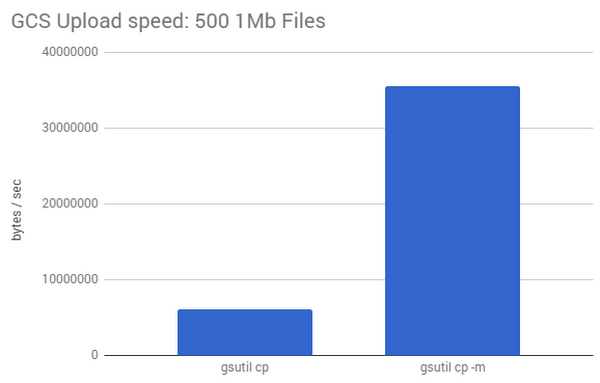
\includegraphics[width=12cm,keepaspectratio]{Pictures/cloud-storage-performance.png}
	\caption{GCS Upload Geschwindigkeit, \citeurl{gcp-blog}}
\end{figure}

Hier sieht man, wie die Leistung sich dabei um das fünffache erhöht im Gegensatz zu den inidivduellen Uploads.\\

Das Auto-balancing von Google Cloud sorgt für die Verteilung der Upload-Connections auf "Backend Shards". Das funktioniert durch die Name/Pfad der Datei und kann die Upload Geschwindigkeit erhöhen, wenn sich die Dateien in unterschiedlichen Ordnern befinden oder auch verschiedene Namensgebungen haben. Falls sich die Dateien zu sehr ähneln, kann dies die Upload Geschwindigkeit reduzieren, da die Connections alle in den gleichen Shard übergehen.\\

Eine weitere Methode, die die Performance steigern kann, sind Requests in Größe ab 1MB. Bei kleineren Requests sollte man die Requests versuchen zu parallelisieren, damit die fixen Latenzkosten überlappen.\\

Es ist zu beachten, dass die Performance auch von anderen Faktoren abhängt, wie die Anwendungsarchitektur, die Netzwerkverbindung und die Implementierung in der Anwendung. Es können spezifische Konfigurationsoptionen genutzt werden, um die Leistung weiter zu optimieren, wie Caching, asynchrone Operationen oder die Nutzung von optimierten Bibliotheken oder Frameworks. 

\newpage

\subsubsection{API Anbindung}

\textbf{Amazon S3}\\

Die API-Anbindung von Amazon S3 ist umfangreich und bietet Entwicklern eine Vielzahl von Möglichkeiten zur Interaktion mit dem Speicherdienst. Amazon S3 bietet eine RESTful API (Application Programming Interface) sowie verschiedene SDKs (Software Development Kits) und Tools, die die Integration und Nutzung erleichtern.\\

Amazon S3 bietet eine RESTful API, die auf dem HTTP-Protokoll basiert. Mit dieser API können Entwickler HTTP-Anfragen wie GET, PUT, POST und DELETE verwenden, um auf Buckets und Objekte in Amazon S3 zuzugreifen, sie zu erstellen, zu lesen, zu aktualisieren und zu löschen. Jedoch empfiehlt Amazon die Nutzung der AWS SDK, da man bei der REST API den nötigen Code für die Kalkulierung der validen Signatur schreiben muss, um sich zu authentifizieren.\glqq It requires you to write the necessary code to calculate a valid signature to authenticate your requests.\grqq, \cite{aws-api}.\\

Die AWS SDK authentifziert Requests durch die Bereitstellung der Access Keys, so fällt das Schreiben des Codes dafür weg. Die SDK ist in verschiedenen Programmiersprachen zugänglich, daruner Java, Javascript, Python, .NET, Ruby, PHP, IOS und Android. Die folgende Tabelle zeigt alle unterstützten Programmiersprachen an.

\begin{figure}[h]
\centering
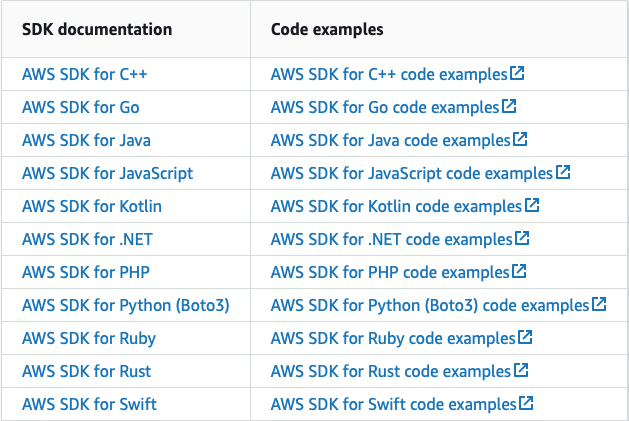
\includegraphics[width=9cm,keepaspectratio]{Pictures/SDKProgrammiersprachen.png}
	\caption{Unterstützte Programmiersprachen von AWS SDK, \citeurl{aws-sdk} }
\end{figure}

Sie bietet eine abstrakte Schnittstelle, um die Entwicklung von Anwendungen zu erleichtern und die Interaktion mit Amazon S3 zu vereinfachen. Darüber hinaus gibt es auch Drittanbieter-Tools und Open-Source Bibliotheken, die die Integration mit Amazon S3 unterstützen. Spring Boot stellt eine Bibliothek für die alte und neue Version von AWS SDK zur Verfügung. Intellij Idea bietet einen Plugin \glqq AWS Toolkit\grqq an, mit dem man seine Amazon Credentials zur Verfügung stellen kann. Diesen Plugin gibt es auch für Eclipse und Visual Studio Code.\\

Außerhalb der AWS SDK stellt Amazon S3 auch die AWS CLI (Command Line Interface) bereit, um API Calls durchzuführen. Amazon S3 ermöglicht die Durchführung von Batch-Operationen, um mehrere Objekte in einem einzigen API-Aufruf zu verarbeiten. Dies erleichtert die effiziente Verarbeitung großer Datenmengen und reduziert die Anzahl der API-Anfragen.\\

Die API-Anbindung von Amazon S3 erfordert eine geeignete Authentifizierung und Autorisierung, um sicherzustellen, dass nur autorisierte Benutzer auf die Daten zugreifen können. Dies erfolgt in der Regel mithilfe von Zugriffsschlüsseln, die über AWS Identity and Access Management (IAM) verwaltet werden.

\newpage

\textbf{Google Cloud Storage}\\

Auch Google Cloud Storage bietet umfangreiche API-Integrationen, um die Einbindung in eigene Anwendungen zu ermöglichen. Eine davon sind die Client Libraries für verschiedene Programmiersprachen wie Java, Python, Node.js, Go, Ruby und .NET. Diese Bibliotheken erleichtern die Integration von Google Cloud Storage in Anwendungen und bieten eine benutzerfreundliche Schnittstelle für die Interaktion mit den Speicherressourcen.\\ Auch in Cloud Storage wird eine RESTful API ähnlich wie in Amazon S3 angeboten. Diese ermöglicht es Entwicklern über HTTP-Anfragen auf die Speicherressourcen zuzugreifen. Sie unterstützt CRUD Operationen für Buckets und Objekte sowie erweiterte Funktionen wie das Setzen von Metadaten, das Verwalten von Zugriffssteuerungen und das Durchführen von Batch-Anfragen.\\

Google Cloud Storage bietet sowohl JSON- als auch XML-APIs für die Interaktion mit dem Speicherdienst. Die JSON-API ist die bevorzugte Option und bietet eine moderne, leichtgewichtige Syntax für die Kommunikation mit dem Dienst anstelle der RESTful API. Neben der direkten API-Anbindung stellt Google auch das Google Cloud SDK zur Verfügung, das verschiedene Befehlszeilentools enthält, mit denen auf Speicherressourcen zugegriffen werden und sie verwalten können. Das SDK bietet auch eine Reihe von Clientbibliotheken für verschiedene Programmiersprachen. Neben den Client-Bibliotheken werden auch Tools wie gsutil (ein Befehlszeilen-Dienstprogramm), das ermöglicht, Cloud Storage von der Befehlszeile aus zu verwalten, sowie Cloud Storage FUSE, das es ermöglicht, Cloud Storage als Dateisystem zu mounten und direkt darauf zuzugreifen.\\

Die API-Anbindung von Google Cloud Storage erfordert ebenfalls eine Authentifizierung und Autorisierung, um sicherzustellen, dass nur autorisierte Benutzer auf die Daten zugreifen können. Dies wird mithilfe von Google Cloud IAM (Identity and Access Management) verwaltet, das Zugriffsrichtlinien und Rollenverwaltung bietet.

\newpage

\subsection{Bereitstellung der Dateien}

In diesem Abschnitt werden Methoden für die Bereitstellung der Dateien durch signierte URL's von Amazon S3 und Google Cloud präsentiert. Unternehmen stehen und Organisationen stehen vor der Herausforderung, Dateien sicher und effizient für ihre Benutzer bereitzustellen. Eine häufig verwendete Methode, um diesen Anforderungen gerecht zu werden, ist die Verwendung von signierten URL's.\\

Signierte URLs ermöglichen es, auf einfache Weise temporäre Zugriffsrechte für Dateien zu gewähren, ohne dass komplexe Zugriffskontrollmechanismen implementiert werden müssen. Sowohl Amazon Web Services (AWS) S3 als auch Google Cloud Storage bieten die Möglichkeit, signierte URLs für die Dateibereitstellung zu generieren.\\

\textbf{Amazon S3}\\

In Amazon S3 sind alle Objekte und Buckets standardmäßig privat. Durch die Verwendung von presigned URLs können Objekte durch Links geteilt werden ohne AWS Sicherheitscredentials.\glqq All objects and buckets are private by default. However, you can use a presigned URL to [...]\grqq, \cite{aws-signed-urls}. 

\begin{quote}
	Presigned URLs werden für die Generierung von Links verwendet, um auf S3 Buckets und Objekte zugreifen zu können. Bei der Erstellung eines solchen URLs können andere Nutzer von außerhalb AWS ohne Credentials auf die gewünschten Daten zugreifen. Jeder der diesen Link hat, kann darauf zugreifen und Aktionen ausführen. Der Link wird bei Konfiguration nach einer bestimmten Zeit die Gültigkeit verlieren. Amazon S3 überprüft das Verfallsdatum des Links während des HTTP Requests, vgl. \cite{aws-signed-urls}. 
\end{quote}

Durch die Nutzung des URL können Nutzer entweder ein Objekt lesen oder ein Objekt hochladen. In dem Fall von leoticket liegt das Lesen des Objekts im Fokus. Die URL beinhaltet spezielle Parameter, welches von einer Anwendung gesetzt werden. Es gibt drei Parameter um den Zugriff für den Nutzer einzuschränken. Diese sind einmal Einschränkung des Buckets. Das bedeutet, das ein Nutzer nicht auf jeden Bucket zugreifen kann, sondern nur auf den Bucket, indem sich das Objekt befindet. Der zweite Parameter ist der Name des Objekts und zuletzt die Zeitspanne in der die URL gültig ist. Sobald die Zeit abgelaufen ist, kann der Nutzer nicht mehr auf den Link zugreifen.\\

Für leoticket bedeutet das, Tickets und Rechnungen nicht mehr als Email-Anhänge bereitstellen zu müssen. Durch die Methode der presigned URLs können diese Links über die Email an die Clients versendet werden.\\

\newpage

\textbf{Google Cloud Storage}\\

In Google Cloud Storage funktioniert die signed URL mit dem ähnlichen Prinzip wie in Amazon S3. Durch zeiteingeschränkte Links können Nutzer, die den Link besitzen, auf Objekte und Buckets zugreifen ohne Google Cloud Credentials. Dabei bietet Cloud Storage mehrere Methoden zur Generierung der Signed URL an. Die V4 signing with service account authentication, Signing with HMAC authentication und die V2 signing with service account authentication. Letztere Methode wird ausgeschlossen, da sie von Google Cloud selbst nicht empfohlen wird. Ein Beispiel wie eine signed URL aussehen kann:

\newpage

\section{Auswahl des Speichersystems}

In diesem Kapitel werden anhand der Anforderungen an leoticket Konfigurationseinstellungen empfohlen. Um der Anforderung der sicheren Speicherung an leoticket zu entsprechen bieten beide Cloud Provider verschiedene Funktionen an, die im vorherigen Kapitel unter Eigenschaften untersucht worden sind. Beide Cloud Provider bieten ähnliche Funktionen für die Erstellung von Benutzern, Gruppen und Rollen um den Zugriff auf die Dienste einzuschränken. Die IAM Funktion bei beiden Cloud Providern ermöglicht es den Zugriff auf S3 und Cloud Storage zu beschränken. Bei der IAM-Funktion in AWS S3 werden einige bewährte Vorgehensweisen empfohlen, um die Sicherheit und den Zugriff auf S3-Ressourcen zu verbessern. Zum einen das Prinzip des geringsten Privilegs. Benutzern und Anwendungen sollten nur die Berechtigungen, die sie zum Durchführen Ihrer Aufgaben benötigen, gewähren. Übermäßige Berechtigungen, um potenzielle Sicherheitsrisiken zu minimieren, sollten vermieden werden. Für leoicket bedeutet dies, wenn eine Anwendung Dateien nach S3 hochladet, dann sollte diese Anwendung nur die benötigten Rechte haben. Dies wären beispielsweise Rechte für das Schreiben und Abrufen von Objekten. Andere Rechte wie beispielsweise das Hinzufügen von Policies können ebenfalls vergeben werden. Diese Empfehlung gilt auch für die IAM Funktion in Google Cloud. Für die Authentifizierung für Anwendungen gibt es Service Accounts, die spezielle Rechte haben, die für die Anwendung relevant sind. Für jeden Dienst oder Anwendung kann ein eigener Service Account erstellt werden.\\

Auch bei der Datenverschlüsselung bieten beide Cloud Provider ähnlichen Möglichkeiten an, mit Encryption Keys umzugehen. Da leoticket eine sichere Speicherung anfordert, kommt die SSE-KMS customer-managed Variante in Frage. Durch die selbstständige Generierung des Schlüssels und Verwaltung, hat der Nutzer mehr Kontrolle im Gegensatz zum S3-managed oder Google-managed Keys. Die generierten Schlüssel werden jedoch bei den Cloud Providern im Key Management Service gespeichert. Wenn für SSE KMS entschieden wurde, kann die Funktion "Bucket Keys" in S3 aktiviert werden. Dadurch hat man einen Master Key, der die Schlüssel der einzelnen Objekte verschlüsselt. Dies reduziert die Request Kosten bis zu 99 Prozent, indem die Request Traffic von S3 zu AWS KMS reduziert wird.\\

Um noch unabhängiger vom Cloud Provider zu sein, kann die Variante customer-supplied in Google Cloud oder die customer-managed Variante in S3 in Frage kommen. Hier hat der Nutzer die volle Verantwortung für die Schlüssel. Das bedeutet, die Schlüssel werden extern vom Nutzer generiert, verwaltet und gespeichert. Dabei besteht das Risiko, den Schlüssel zu verlieren und nicht mehr auf die Objekte in S3 zugreifen zu können. Außerdem ist der Aufwand für die selbstständige Verwaltung des Schlüssels höher als die Verwendung des KMS.\\

Beide Cloud Provider bieten die Möglichkeit, ACLs auf Objekte anzuwenden. Das bedeutet, das für jedes Objekt Zugriffskontrollen eingestellt werden. Jedoch wird bei beiden Cloud Providern empfohlen diese Einstellung deaktiviert zu lassen und nur bei besonderen Fällen zu verwenden.\\

Für die Sicherheit und Verfügbarkeit der Daten wird empfohlen Object Versioning zu aktivieren, um mehrere Versionen von Objekten bereitzustellen. Dies kann Objekte beim versehentlichen Löschen oder Überschreiben wiederhergestellt werden. Beide Cloud Provider bieten diese Funktion beim Erstellen eines Buckets an. AWS und Google Cloud bieten eine Auswahl von Speicherklassen zur Verfügung. Beide Provider versprechen eine Verfügbarkeit von mindestens 99.9 Prozent. Die Speicherklasse Standard-Infrequent Access von S3 und Nearline von Cloud Storage können für leoticket empfohlen werden. Da in leoticket die Anforderungen an das Abrufen von Dateien innerhalb Millisekunden liegt, fallen die Speicherklassen von S3 Glacier weg, da das Abrufen von Dateien Tage oder Stunden dauern kann. Die Daten in leoticket müssen auf Abruf zur Verfügung stehen, jedoch wird davon ausgegangen, das Objekte im Durchschnitt zweimal abgerufen werden. Einmal von der Anwendung und einmal von den Kunden, die die Tickets gekauft haben. Durch die geringe Abrufanzahl eines einzelnen Objekts und die 10 Jahre Speicherung von Daten kommen die Speicherklassen Standard-IA und Nearline in Frage. Diese Speicherklassen sind für Daten geeignet, auf die weniger häufig zugegriffen werden, aber bei Bedarf schnell verfügbar sein müssen. Sie bieten gleichzeitig eine kostengünstigere Option für die Speicherung der Daten. Die One Zone-IA von S3 speichert die Daten in nur einer AZ und wird aufgrund des Risikos der Verringerung der Verfügbarkeit bei Ausfall der AZ nicht empfohlen. Dadurch kann das Abrufen der Daten länger dauern. Die Coldline Speicherklasse von Google Cloud kann in Frage kommen, wenn Daten für eine sehr lange Zeit nicht mehr abgerufen worden sind und auch in nächster Zeit nicht mehr zugegriffen werden wird. Denn die Coldline ist für Daten ausgelegt, auf die selten zugegriffen werden und bei denen eine längere Zugriffszeit akzeptabel ist.  Sie eignet sich gut für die Archivierung.\\

Bei der API Integration unterscheiden sich die beiden Provider in wenigen Punkten. Für leoticket ist es wichtig, dass die API in die leoticket Anwendung integrierbar ist, ohne viel Aufwand. Dies ist bei beiden Providern der Fall, denn beide bieten SDKs, CLIs und REST APIs an, die leicht in die eigene Anwendung integrierbar sind. Frameworks wie Spring Boot bieten Dependencies zu der AWS SDK Version 1 und 2 und auch für Google Cloud an. AWS hat den Vorteil, dass On-Premise Anwendungen wie MinIO die AWS API verwendet und so eine S3-Kompatibilität verschafft. Dies hat den Vorteil, dass man sich bereits mit der API auskennt und über MinIO Dateien nach S3 hochladen und herunterladen kann. Dies ist zwar auch über Google Cloud möglich, aber wenn man sich noch nicht mit der AWS API auskennt, ist es nötig sich in die Technologie einzuarbeiten. Um sich mit der API authentifizieren zu können ist es empfehlenswert bei der Google SDK Service Accounts zu verwenden. Jedoch gibt es auch andere Methoden zur Authentifizerung.  Über die ADC in Google Cloud kann entschieden werden mit welcher Methode authentifziert wird. AWS bietet für die Authentifzierung das \glqq AWS Toolkit \grqq an, dass von IntelliJ, Eclipse und anderen IDEs unterstützt wird. Über das Toolkit ist die Authentifzierung empfohlen.\\

Um die beste Performance für leoticket zu gewährleisten ist es ratsam, Performance Analysen durchzuführen. Dafür gibt es Tools, die AWS und Google Cloud anbieten. Bei Google Cloud kann man mit dem "gsutil" CLI eine Performance Diagnose durchführen. Dies muss auch durchgeführt werden, wenn man den Support von Google Cloud kontaktiert, um eine Fehlerbehebung zu finden. AWS bietet in diesem Punkt Metrics direkt in dem S3 Bucket an. Es werden verschiedene Widgets für Request Metrics bereitgestellt, die man analysieren kann. Im Kapitel "Prototypische Umsetzung" werden Messungen für die Performance Analyse durchgeführt und anschließend analysiert, um die beiden Cloud Anbieter in diesem Punkt besser vergleichen zu können.\\ 

Die Entscheidung zwischen den Cloud Providern liegt sowohl an den Anforderungen an leoticket als auch an den Präferenzen der Entwickler. Wenn sich Entwickler bereits mit einem Cloud Provider auskennen und beschäftigt haben, dann ist es ratsam sich für diesen Provider zu entscheiden. Dies hat den Vorteil, dass man sich nicht auf eine neue Technologie einarbeiten muss und Zeit sparen kann bei der Implementierung und Integration der API. Es ist legitim zu sagen, das beide Anbieter viele Funktionen und ähnliche Produkte anbieten, die auf die Anforderungen von Leoticket angepasst werden können. Diese Arbeit dient lediglich dazu, eine Hilfestellung bei der Entscheidung zu sein, um sich am Ende für eines entscheiden zu können. 

\newpage

\subsection{Kostenanalyse}

Bei der Kostenanalyse werden die Gebühren aus dem Kosten Abschnitt übernommen und eine Kostenabschätzung für Amazon S3 und Cloud Storage durchgeführt. Es werden die Kosten für die Speicherung, Abrufen und Datenübertragung verglichen und dargestellt. Die Berechnungsdaten stammen aus leoticket und dienen der groben Kosteneinschätzung. Die Kosten können von verschiedenen Faktoren voneinander abweichen. Der aktuelle Stand der Kosten ist gleich dem Abgabedatum der Arbeit.\\

Für die grobe Einschätzung der Kosten wird von 800 000 Bestellungen im Durchschnitt über leoticket pro Jahr ausgegangen. Pro Monat sind das ca. 67 000 Bestellungen mit jeweils 4 Objekten pro Bestellung. Die Größe eines Objektes beträgt dabei im Durchschnitt 100kb. Pro Bestellung werden im Durchschnitt drei Tickets gekauft, wobei noch eine Rechnung hinzugefügt wird. Diese 4 Objekte machen eine Bestellung mit insgesamt 400kb aus. Es wird davon ausgegangen, dass es monatlich ungefähr 67 000 POST Requests nach Amazon S3 verschickt werden. Außerdem wird davon ausgegangen, dass Objekte jeweils zweimal im Monat abgerufen werden können. Einmal von Leomedia und von den Kunden aus. Insgesamt werden es 134 000 GET Requests von Amazon S3 aus geben.\\

Die Speichergröße ergibt sich aus den 67 000 Bestellungen pro Monat mal die 400kb Größe pro Bestellung. Diese werden geteilt durch 1024 und das Ergebnis nochmal durch 1024 um die GB Einheit zu bekommmen. Das ergibt 25GB pro Monat an Speicher. Wenn man die Retention von 10 Jahren dabei bedenkt, dann sind das ungefähr 3TB Daten die gespeichert werden müssen, wenn Daten erst nach 10 Jahren gelöscht werden. Mit diesen gewonnen Daten werden die Preisrechner von AWS und Google Cloud verwendet und die entsprechenden Daten eingesetzt.\\

%TODO Preisrechner Links hier einsetzen

\textbf{Amazon S3}\\

Im Folgenden wird die folgende Tabelle bereitgestellt, um die Kosten für die verschiedenen Speicherklassen darzustellen.

\begin{figure}[h]
\centering
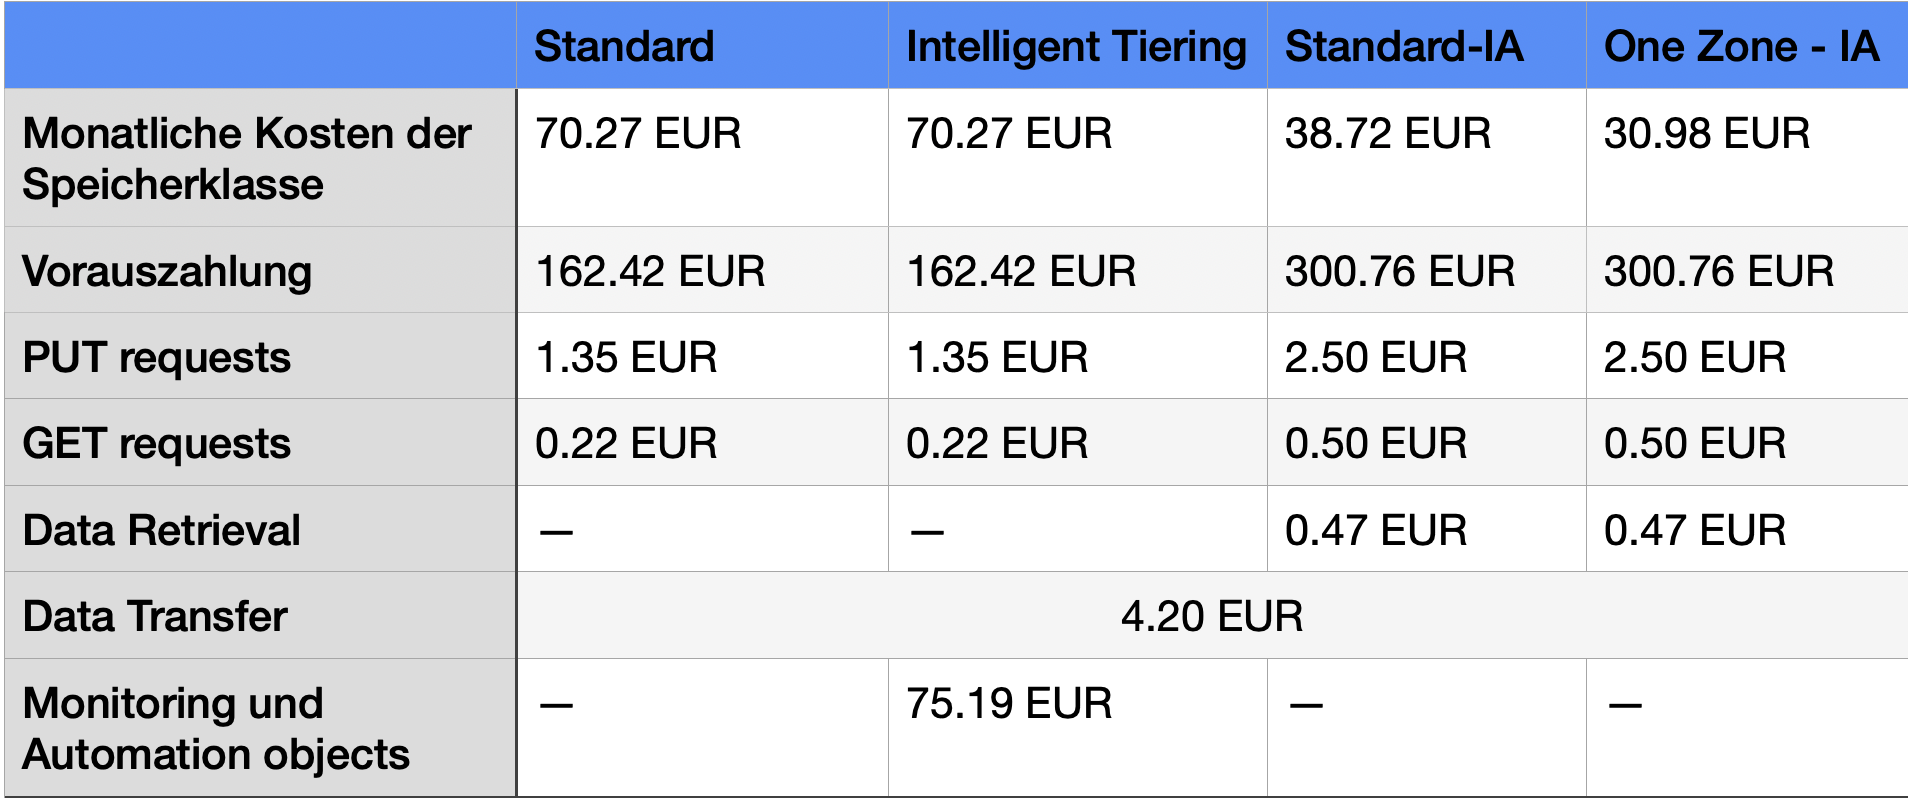
\includegraphics[width=12cm,keepaspectratio]{Pictures/AWSKostenOhneGesamt.png}
\caption{Gesamtkosten der Datenspeicherung in Amazon S3}	
\end{figure}

Zuerst werden die Einheitsumwandlungen durchgeführt. Dabei werden die angegebenen 3TB im Monat mal die 1024GB multipliziert, um die exakte Menge an GB auszurechnen. Dies ist bei 3072GB. Danach wird die Objektgröße von 400kb in GB umgerechnet, was 0.000095367432 GB ergibt. Anschließend werden die Preise kalkuliert. 

\newpage

\begin{align}
	\frac{3072 \text{ GB per Month}}{0.000381469728 \text{ GB average item size}} = 8.053.064 \text{ number of objects}\\
	3072 \text{ GB} \times 0.0135 \text{ USD} = \text{41.472 USD Standard-IA costs}\\
	67.000 \text{ PUT requests} \times 0.00001 \text{ USD per request} = 0.67 \text{ USD (PUT requests cost)}\\
	134.000 \text{ GET requests} \times 0.000001 \text{ USD per request} = 0.134 \text{ USD (GET requests cost)}\\
	50 \text{ GB} \times 0.01 \text{ USD} = 0.50 \text{ USD (data retrievals cost)}\\
	41.472 \text{ USD} + 0.67 \text{ USD} + 0.134 \text{ USD} + 0.50 \text{ USD} = \underline{\textbf{42.78  USD (Total Standard-IA)}}\\
	8.053.064 \text{ number of objects} \times 0.00001 \text{ USD} \\ = \text{80.53 USD (Cost for PUT, COPY, POST requests for initial data)}
\end{align}

Die obigen Formeln sind ähnlich wie bei der Standard und One Zone-IA, wenn man dabei die jeweiligen Gebühren aus dem Kosten Abschnitt übernimmt. Bei der Intelligent Tiering gibt es noch den Unterschied, dass die Kosten für Monitoring und Automation dazu kommt und die Einteilung des Speichers in Prozent auf drei Speicherklassen. In der letzten Zeile der abgebildeten Tabelle werden die Gesamtkosten gemeinsam mit den Kosten des Datentransfers, Vorauszahlung und die puren monatlichen Speicherkosten der jeweiligen Speicherklassen addiert.\\

\textbf{Google Cloud Storage}\\

In der folgenden Tabelle werden die Kosten von Google Cloud Storage für drei Speicherklassen zusammengefasst:

\begin{figure}[h]
\centering
	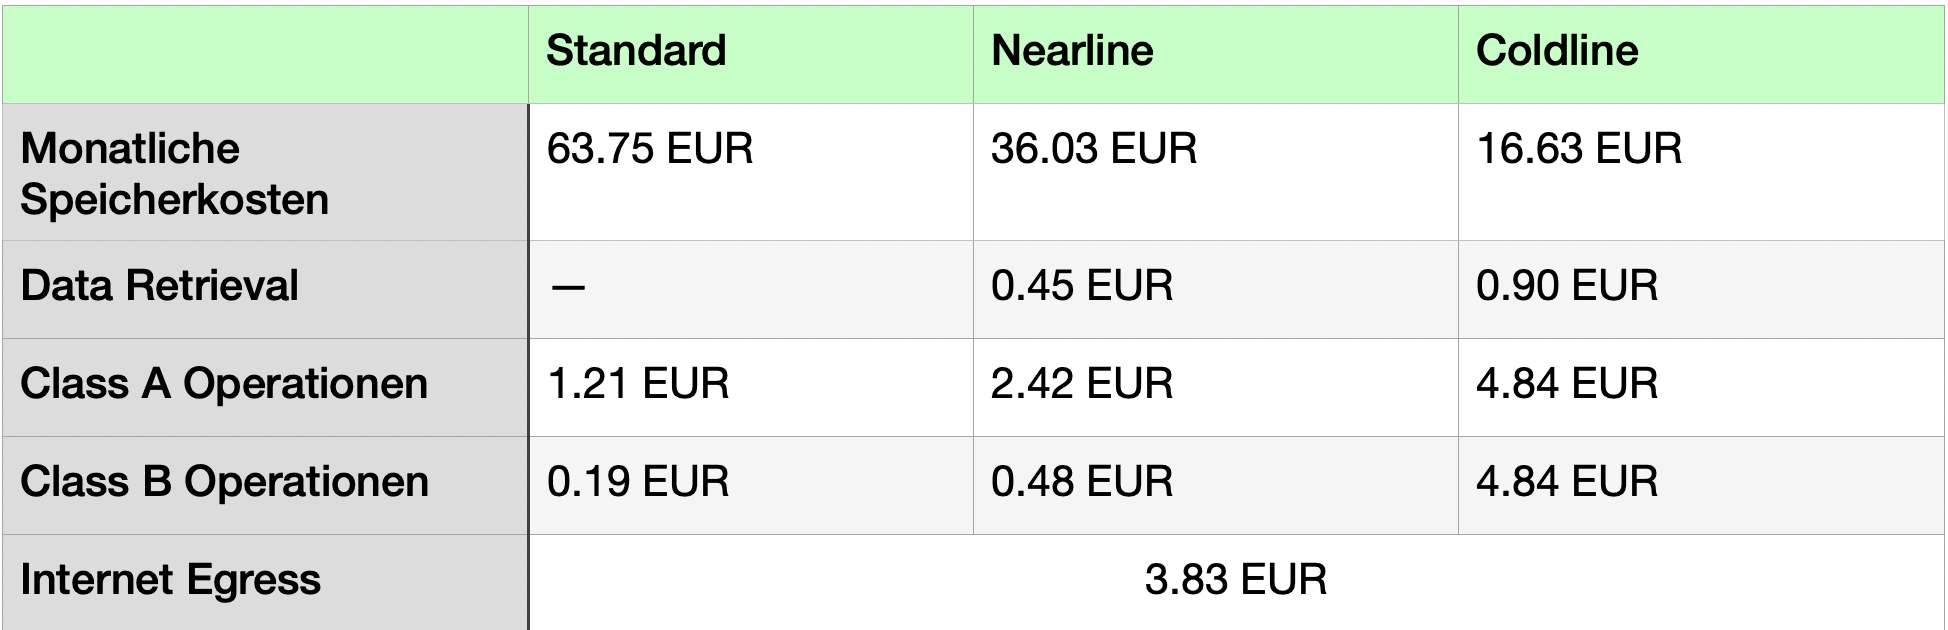
\includegraphics[width=12cm,keepaspectratio]{Pictures/GCKostenOhneGesamt.png}
	\caption{Gesamtkosten der Datenspeicherung in Google Cloud Storage}
\end{figure}

Die teuerste Speicherklasse mit 64.10 Euro ist die Standard Klasse. Die billigste mit 16.63 Euro ist die Coldline Klasse. Die Nearline Speicherklasse ist mit 36.03 Euro teurer als die Coldline. Bei der Standard Klasse gibt es keine Gebühren für die Daten Retrieval.
\chapter{Prototypische Umsetzung}     

Im folgenden Kapitel wird der Prototyp genauer betrachtet und die verschiedenen Aspekte seiner Entwicklung und Implementierung werden erläutert. Es werden dabei die verwendeten Technologien und die Art der Speicherung und Bereitstellung von Binärdaten beleuchtet. Um die Performance zu bewerten, werden Messungen auf generierte Testdaten durchgeführt. Insgesamt dient das Kapitel als Grundlage für weitere Untersuchungen und die Optimierung des Prototyps.\\                               

\section{Überblick und Vorgehensweise}

Zunächst wird auf die eingesetzten Technologien eingegangen, die bei der Entwicklung des Prototyps verwendet werden. Dies umfasst das Framework Spring Boot und Programmiersprachen, die zur Umsetzung des Prototyps genutzt werden. Ein besonderes Augenmerk wird auf die Speicherung der Binärdaten gelegt. Hier werden verschiedene Ansätze betrachtet, wie beispielsweise die Verwendung von dem AWS SDK und der Google Client Libraries. Des Weiteren wird die Bereitstellung der Binärdaten behandelt. Hier wird die Methode der Signed URLs betrachtet, um die Daten effizient an die Anwender zu übertragen. Um die Leistung des Prototyps zu bewerten, werden Testdaten mit zufälligem Inhalt generiert. Dies ermöglicht eine realistische Simulation der Tickets und Rechnungen in leoticket und erlaubt eine Bewertung der Performance der Cloud Provider. Die Messungen werden auf einem virtuellen Server durchgeführt, um eine isolierte Umgebung zu gewährleisten. Dies ermöglicht es, Performance Messungen unabhängig von anderen Prozessen oder Anwendungen auf dem Host-System durchzuführen, ohne Störungen zu verursachen.\\

\newpage

\section{Eingesetzte Technologien}

Für die Umsetzung des Prototyps werden die folgenden Technologien eingesetzt:

\begin{itemize}
	\item Spring Boot v3
	\item AWS SDK 2.0 Version
	\item GC Storage client library
	\item Java SDK v17
	\item Apache Maven v3.9.1
	\item Maven Schema v4.0.0
	\item AWS Toolkit
	\item aws cli
	\item gcloud cli
\end{itemize}

Für die Implementierung wurde die Entwicklungsumgebung IntelliJ IDEA Ultimate verwendet. IntelliJ bietet ein Plugin namens \verb|AWS Toolkit| an. Als Framework wurde die aktuellste Version von Spring Boot (Version 3) zum Zeitpunkt der Erstellung des Prototyps verwendet. Spring Boot stellt SDKs beider Cloud-Provider als Maven-Abhängigkeiten zur Verfügung.

\begin{quote}
	Am 17. März 2021 wurde die neue Version des Spring Cloud AWS 2.3 veröffentlicht. Spring Cloud GCP und Spring Cloud AWS sind nicht mehr Teil des Spring Cloud Releases. Nicht Teil des Releases zu sein bedeutet auch, dass sie aus der Spring Cloud Organisation auf Github herausgenommen worden sind und dadurch neue Maven Package Namen haben. Das neue Package für Spring Cloud AWS heißt nun \glqq io.awspring.cloud\grqq, vgl. \cite{spring-cloud}. 
\end{quote}

Die unten aufgeführten Maven Abhängigkeiten werden für AWS S3 und Cloud Storage verwendet:

\begin{lstlisting}[language=XML]
	<dependency>
        	<groupId>com.google.cloud</groupId>
        	<artifactId>spring-cloud-gcp-starter-storage</artifactId>
    </dependency>
\end{lstlisting}

\begin{lstlisting}[language=XML]
	dependency>
        	<groupId>io.awspring.cloud</groupId>
        	<artifactId>spring-cloud-aws-s3</artifactId>
        	<version>3.0.0</version>
    </dependency>
\end{lstlisting}

Als Spring Cloud GCP Version wird die 4.2.0 verwendet. Beide Spring Cloud Abhängigkeien werden von der Community auf Github verwaltet und aktualisiert. Für die Erstellung des Spring Boot Projekts wurde der Spring Initializier von Spring selbst verwendet (\url{https://start.spring.io/}). Zudem wird das Java SDK Version 17 verwendet. Für Apache Maven wird die Version 3.9.1 verwendet. Das Listing 8.1 im Anhang beinhaltet die vollständige pom.xml Datei, in der die Abhängigkeiten des Prototyps dargestellt werden.

Für die Authentifizierung wird das \verb|gloud| cli verwendet. Dieses wird über die offizielle Dokumentation installiert. Siehe \url{https://cloud.google.com/sdk/docs/install?hl=de}. Das AWS Toolkit wird für die Authentifizierung mit AWS angewendet. Um sich mit GC zu verbinden wird eine Methode des ADC verwendet, welches im nächsten Abschnitt genauer erläutert wird.

\newpage

\section{Speicherung von Binärdaten}

Um Daten in S3 oder Cloud Storage speichern zu können, wurde der Prototyp so implementiert, dass der Nutzer sich zwischen S3 oder Cloud Storage entscheiden kann. Dies geschieht über die Klasse \verb|CloudStorageServiceFactory|, (siehe Listing 8.3 im Anhang). Hier kann der Nutzer über die Umgebungsvariable \verb|cloud_provider| den gewünschten Provider mit \verb|aws| oder \verb|google cloud| angeben. Dabei wird die Groß-, und Kleinschreibung nicht berücksichtigt. Die Umgebungsvariablen können unter Linux, OSX und Unix im System durch \verb|export <EnvironmentVariable>=<value>| exportiert werden. Wenn eine IDE wie Intellij verwendet wird, können sie unter den Run-Einstellungen eingefügt werden. Nach der Eingabe des Cloud Providers wird das Programm die entsprechende Klasse aufrufen. Für AWS die Klasse \verb|AWSS3StorageService| und für GC die Klasse \verb|GCStorageService|. Beide Klassen implementieren das Interface \verb|CloudStorageService|. Dieses definiert zwei Methoden, die zum Hoch- und Herunterladen der Daten zuständig sind:

\begin{lstlisting}[language=Java]
void uploadObject(String bucketName, String key, String file, String encryptionKey, String storageClass) throws IOException;
\end{lstlisting}

\begin{lstlisting}[language=Java]
URL getPresignedUrl(String bucketName, String key, Integer minutes, String encryptionKey);
\end{lstlisting}
	
Der \verb|uploadObject| Methode wird der Bucket Name, der Name des Objekts, der Pfad des Objekts und der Encryption Key übergeben. Der Encryption Key kann dabei der Schlüssel sein, der in AWS KMS oder GC KMS generiert wurde. Die Implementierung dieser Methode ist für beide Cloud Provider ähnlich gestaltet.

\begin{lstlisting}[language=Java, caption=Prototyp Code Snippet - Hochladen eines Objekts nach S3]
@Override
public void uploadObject(String bucketName, String key, String file, String encryptionKey, String storageClass) {
    try {

(1)     PutObjectRequest putObjectRequest = PutObjectRequest.builder()
(2)             .bucket(bucketName)
(3)             .key(key)
(4)             .serverSideEncryption(ServerSideEncryption.AWS_KMS)
(4)             .ssekmsKeyId(encryptionKey)
(5)             .storageClass(storageClass)
                .build();

(6)     Path filePath = Paths.get(file);
(7)     byte[] fileBytes = Files.readAllBytes(filePath);
(8)     RequestBody requestBody = RequestBody.fromBytes(fileBytes);

(9)     this.s3Client.putObject(putObjectRequest, requestBody);
        logger.info(
        "File " + file + " uploaded to bucket " + bucketName + " as " + key
        );

    } catch (S3Exception | IOException e) {
        logger.error(e.getMessage());
    }
}
\end{lstlisting}

\newpage

Der vorliegende Code (3.1) beschreibt den Vorgang des Speicherns eines Objekts in AWS S3. Zunächst wird ein PUT-Request-Objekt erstellt (1), wobei Parameter wie der Bucket-Name (2), der Objektname als Key (3) und die Authentifizierungsmethoden (4) angegeben werden. Dabei wird die AWS KMS-Methode verwendet und der entsprechende Schlüssel bereitgestellt (4). Anschließend wird die Speicherklasse angegeben, in der das Objekt gespeichert werden soll (5). In diesem Beispiel wird die Standard-IA-Klasse verwendet. Danach wird der Pfad der angegebenen Datei gelesen (6), in ein Byte-Array umgewandelt (7) und dem \verb|RequestBody| übergeben (8). Der RequestBody wird mit dem \verb|PutObjectRequest| an den \verb|S3Client| übergeben und mit der AWS \verb|.putObject()| Methode in S3 hochgeladen (9). AWS S3 verschlüsselt das Objekt mit dem angegebenen Schlüssel und lädt es in S3 hoch.\\

Das folgende Code Snippet zeigt die Methode der Klasse \verb|GCStorageService|. Ähnlich wie bei der Methode für AWS S3 wird auch hier ein Objekt nach Cloud Storage hochgeladen:

\begin{lstlisting}[language=Java, caption=Prototyp Code Snippet - Hochladen eines Objekts nach Cloud Storage]
@Override
public void uploadObject(String bucketName, String key, String file, String encryptionKey, String storageClass) throws IOException {

    Map<String, String> kmsKeyName = new HashMap<>();
    kmsKeyName.put("kmsKeyName", encryptionKey);

    // Get a reference to the bucket
(1) BlobId blobId = BlobId.of(bucketName, key);
(2) BlobInfo blobInfo = BlobInfo.newBuilder(blobId)
            .setMetadata(kmsKeyName)
            .build();

    Storage.BlobWriteOption precondition;
    if (this.storage.get(bucketName, key) == null) {
        precondition = Storage.BlobWriteOption.doesNotExist();
    } else {
        precondition =
                Storage.BlobWriteOption.generationMatch(
                        this.storage.get(bucketName, key).getGeneration());
    }
(3) this.storage.createFrom(blobInfo, Paths.get(file), precondition);

    logger.info(
    "File " + file + " uploaded to bucket " + bucketName + " as " + key
    );

}
\end{lstlisting}

Dabei werden ähnliche Parameter der Methode wie in AWS S3 übergeben. Um ein Objekt in einen Bucket hochladen zu können, wird eine Referenz zu diesem erstellt. Dies geschieht durch die \verb|BlobId|, welche den Bucket Namen und den Namen des Objekts beinhaltet (1). 
Anschließend wird diese blobId dem \verb|BlobInfo| Objekt übergeben und der Encryption Key über die Metadaten \verb|kmsKeyName| gesetzt (2). Nachdem überprüft worden ist, ob das Objekt bereits im Bucket existiert, wird das Objekt hochgeladen (3).\\

Um das Programm auszuführen, wird die Hauptklasse \verb|CloudGcStorageAwsS3Application| gestartet. Damit das Programm erfolgreich läuft, müssen die Umgebungsvariablen im System exportiert werden. Alle Umgebungsvariablen sind in der \verb|application.properties| hinterlegt, (siehe Listing 8.2 im Anhang). Diese werden beim Start des Programms gelesen und angewendet. Außerdem müssen die AWS und GC Credentials hinterlegt werden. Dies kann entweder über das AWS Toolkit Plugin gesteuert werden oder in der Kommandozeile mit dem Befehl \verb|aws configure|. Für GC Credentials kann mit dem Befehl:\\ \verb|export GOOGLE_APPLICATION_CREDENTIALS=<service-account-json-file>| der Service Account hinterlegt werden oder durch Ausführen des Befehls \verb|gcloud auth application-default login| in der Kommandozeile, was die Credentials lokal speichert und für ADC verwendet wird.

\newpage

\section{Bereitstellung der Binärdaten}

Bei der Bereitstellung von Binärdaten in leoticket geht es darum, den Kunden Dateien über Links zugänglich zu machen. Hierfür werden signierte URLs verwendet. Im folgenden Abschnitt werden die Implementierungen und Erläuterungen des entsprechenden Codes von beiden Cloud Providern vorgestellt.\\

Folgender Code Snippet (3.3) zeigt die Methode \verb|getPresignedUrl| zur Generierung einer signierten URL der Klasse \textbf{AWSS3StorageService}:

\begin{lstlisting}[language=Java, caption=Prototyp Code Snippet - Generierung einer signierten URL durch AWS]
@Override
public URL getPresignedUrl(String bucket, String key, Integer minutes, String encryptionKey) {
    try {

(1)     GetObjectRequest getObjectRequest = 
			GetObjectRequest.builder()
(2)             .bucket(bucket)
(3)             .key(key)
                .build();

        GetObjectPresignRequest getObjectPresignRequest =                  
             GetObjectPresignRequest.builder()
(4)             .getObjectRequest(getObjectRequest)
(5)             .signatureDuration(Duration.ofMinutes(minutes))
                .build();

        PresignedGetObjectRequest presignedGetObjectRequest =                  
(6)          presigner.presignGetObject(getObjectPresignRequest);

(7)     URL url = presignedGetObjectRequest.url();

        logger.info("Presigned URL: " + url);

        return url;

    } catch (S3Exception e) {
        logger.error(e.getMessage());
    }

    return null;
}
\end{lstlisting}

Die Methode erhält ähnlich wie beim Hochladen des Objekts die Parameter Bucket-Name und Objektname. Zudem wird eine Zeitdauer in Minuten übergeben, die festlegt, wie lange der generierte Link gültig sein soll. Für die Entschlüsselung der Daten muss der gleiche Encryption Key wie beim Hochladen verwendet werden. Das \verb|GetObjectRequest| Objekt wird erstellt (1) und mit dem Bucket-Namen (2) und dem Objektnamen (3) versehen. Anschließend wird dieses Objekt an das \verb|GetObjectPresignRequest| Objekt übergeben (4) und die Gültigkeitsdauer der Signatur angegeben (5). Diese bestimmt, wie lange die signierte URL valide ist.\\

Um die signierte URL zu generieren, wird das \verb|GetObjectPresignRequest| Objekt an den \verb|S3Presigner| übergeben (6), auf welche die Methode \verb|presignGetObject()| aufgerufen wird (6). Das generierte \verb|PresignedGetObjectRequest| wird als URL gespeichert (7) und ausgegeben.\\

Folgende Abbildung zeigt die Methode zur Generierung einer signierten URL der \\Klasse \verb|GCStorageService|:

\begin{lstlisting}[language=Java, caption=Prototyp Code Snippet - Generierung einer signierten URL durch GC]
@Override
public URL getPresignedUrl(String bucketName, String key, Integer minutes, String encryptionKey) {
    try {
        Map<String, String> kmsKeyName = new HashMap<>();
        kmsKeyName.put("kmsKeyName", encryptionKey);

        // Define resource
(1)     BlobInfo blobInfo = BlobInfo.newBuilder(BlobId.of(bucketName, key))
                .setMetadata(kmsKeyName)
                .build();

(2)     URL url = this.storage.signUrl(
(3)             blobInfo,
(4)             minutes,
                TimeUnit.MINUTES,
(5)             Storage.SignUrlOption.withV4Signature()
        );

        logger.info("Generated GET signed URL: " + url);

(6)     return url;

    } catch (StorageException e) {
        logger.error(e.getMessage());
    }

    return null;
}
\end{lstlisting}

Ähnlich wie bei S3 wird eine Referenz zum Objekt erstellt, indem der Bucket Name und der Name des Objekts dem \verb|BlobInfo| Objekt mitgegeben wird (1). Anschließend kann die URL durch Aufrufen der Methode \verb|.signUrl()| erstellt werden (2). Hier werden das \verb|BlobInfo| Objekt (3), die Minuten (4) und die Signatur Methode (5) übergeben. Zuletzt wird die URL ausgegeben (6).\\

Mit signierten URLs können die Anforderungen von leoticket an die sichere Speicherung und Bereitstellung der Daten berücksichtigt werden. Dies bedeutet, Kunden können über diese Links, die durch Emails versendet werden, die Dateien für Tickets und Rechnungen herunterladen. Die Herausforderung von leoticket, große Email-Anhänge zu versenden, kann vermieden werden.\\

\newpage

\section{Messung der Performance}

In diesem Abschnitt erfolgt die Messung der Performance für die Dienste von AWS und GC. Dabei werden bis zu 1000 generierte Dateien sowohl für den Upload als auch für den Download betrachtet. Die Performance Analyse wird auf einer virtuellen Maschine in der Hetzner Cloud ausgeführt, um eine isolierte Umgebung zu gewährleisten. Die Performance-Messung beim Hoch- und Herunterladen kann jedoch von verschiedenen Faktoren wie Netzwerklatenz, verfügbarer Bandbreite, Serverkapazität, Datenmenge und der Auslastung der Server beeinflusst werden. Außerdem kann der Hetzner Server näher an AWS oder GC liegen und dies könnte dazu führen, dass die Dauer des Hoch- und Herunterladens aus diesem Grund kürzer ist. Die Messungen dienen lediglich dem groben Vergleich beider Cloud Provider. Die Performance-Messung wird auf verschiedene Speicherklassen durchgeführt, um einen Vergleich zwischen diesen zu ermöglichen und eine Grundlage für die Bewertung ihrer Leistungsfähigkeit zu schaffen.\\

\textbf{AWS}\\

AWS bietet Dienste für die Performance Analyse. Unter anderem die Amazon CloudWatch, S3 Storage Lens und die S3 Transfer Acceleration. Die AWS CLI stellt einfache Methoden zum S3 Upload und Download Tests vor. Beispielsweise kann man mit dem Befehl:

\begin{lstlisting}
	aws s3 cp <lokaler_pfad> s3://<Bucket_Name>/<Ziel_Dateipfad>
\end{lstlisting}

Dateien hoch- und herunterladen und die Zeit für die benötigte Request messen. Auch mit dem AWS SDK können Performance Test Skripte geschrieben werden. Diese Methode wird für den Prototypen angewendet. Dabei werden Tests bereitgestellt, die mehrere Dateien automatisch hoch- und herunterladen und dabei die vergangene Zeit messen.\\ 

\textbf{GC Storage}\\

GC bietet ein eigenes \verb|gsutil| Tool für die Performance Analyse. Wie im Abschnitt Performance bereits erwähnt, können durch die \verb|perfdiag| Funktion Performance Diagnosen erstellt werden.\\ 

Mehrere Testdateien werden aus einem angegebenen Bucket hoch- und heruntergeladen. Nach der Analyse werden alle Testdateien nach erfolgreicher Diagnose gelöscht. Die \verb|gsutil| Performance kann von Faktoren wie vom Client, Server oder Netzwerk beeinflusst werden. Möglich sind die Leistung, der verfügbare Speicher, die Netzwerk Bandbreite, Firewalls und Fehlerraten zwischen \verb|gsutil| und den Google Servern. Die \verb|perfiag| Funktion wurde bereitgestellt, damit Nutzer Messungen durchführen können, die beim Troubleshooting von Performance Problemen helfen, vgl. \cite{gc-perfdiag}.

\newpage

Um die Performance Diagnose auszuführen, kann der folgende Befehl verwendet werden:

\begin{lstlisting}
	gsutil perfdiag -o test.json -n 67000 -s 400kb gs://leoticket-bucket
\end{lstlisting}

Die \verb|-o| Option schreibt den Output des Ergebnisses in eine Datei. Die Output Datei ist eine JSON Datei mit System Informationen und enthält die Performance Diagnose Ergebnisse. Die -n Option setzt die Anzahl der Objekte, die heruntergeladen und hochgeladen werden sollen während des Tests. Mit der \verb|-s| Option kann man die Objektgröße angeben. Zum Schluss wird der Name des Buckets angegeben.\\

Um die Performance der SDKs zu analysieren, werden Objekte mit jeweils 100 KB Objektgröße in verschiedenen Speicherklassen hoch- und heruntergeladen. Anschließend wird die Performance über das SDK von Cloud Storage ähnlich wie bei AWS getestet. Der Test wird ebenfalls auf einer virtuellen Maschine von Hetzner ausgeführt.\\

Die Performance wird in Zehner-Vielfachen gemessen, beginnend mit einer Datei bis hin zu 1000 Dateien. Dies bedeutet, dass Messungen für eine Datei, zehn Dateien, 100 Dateien und 1000 Dateien durchgeführt werden. Zur Durchführung der Messung wird eine Jar Datei des Prototyps erstellt, in der die Testmethoden (siehe Listing 8.4 bis 8.8 im Anhang) ausgeführt werden. Diese generieren zunächst Testdaten, die mit zufälligen String-Werten der Größe 100 KB gefüllt werden, (siehe Listing 8.9 und 8.10 im Anhang). Anschließend werden die Testmethoden in der Kommandozeile ausgeführt. 

\newpage

\subsection{Messungsergebnisse}

In diesem Abschnitt werden die Messungsergebnisse der Performance Messung in Millisekunden präsentiert. Die Speicherklassen Standard, Standard-IA und One Zone-IA von AWS wurden jeweils mit Standard, Nearline und Coldline von GC verglichen. Im Folgenden werden die Ergebnisse der Upload und Download Dauer aller Speicherklassen präsentiert: 

\begin{table}[!h]
\centering
\begin{tabular}{ |s|p{3cm}|p{3cm}| }
\hline
\rowcolor{pink!35}
 & \textbf{Standard-IA} & \textbf{Nearline}\\
\hline
\textbf{1 Datei} &  &  \\
Upload & 705 & 841 \\
Download   &  18 & 26 \\
\textbf{10 Dateien}  & &  \\
Upload & 1862 & 3217\\
Download   &  35 & 94 \\
\textbf{100 Dateien}  & &  \\
Upload & 16681 & 22683\\
Download   &  129 & 269 \\
\textbf{1000 Dateien}  & & \\
Upload & 71175 & 185134\\
Download   &  663 & 1489 \\
\hline
\end{tabular}
\caption{Ergebnisse der Upload und Download Dauer der Speicherklassen Standard-IA und Nearline}
\end{table}


\begin{table}[!h]
\centering
\begin{tabular}{ |s|p{3cm}|p{3cm}| }
\hline
\rowcolor{pink!35}
 & \textbf{Standard S3} & \textbf{Standard GCS}\\
\hline
\textbf{1 Datei} &  &  \\
Upload & 585 & 660 \\
Download   &  28 & 19 \\
\textbf{10 Dateien}  & &  \\
Upload & 1369 & 3002\\
Download   &  70 & 108 \\
\textbf{100 Dateien}  & &  \\
Upload & 8110 & 20750\\
Download   &  180 & 396 \\
\textbf{1000 Dateien}  & & \\
Upload & 73992 & 176004\\
Download   &  650 & 1619 \\
\hline
\end{tabular}
\caption{Ergebnisse der Upload und Download Dauer der Speicherklassen Standard S3 und Standard GCS}
\end{table}

\newpage

\begin{table}[!h]
\centering
\begin{tabular}{ |s|p{3cm}|p{3cm}| }
\hline
\rowcolor{pink!35}
 & \textbf{OneZone-IA} & \textbf{Coldline}\\
\hline
\textbf{1 Datei} &  &  \\
Upload & 505 & 636 \\
Download   &  28 & 18 \\
\textbf{10 Dateien}  & &  \\
Upload & 1105 & 2855\\
Download   &  65 & 89 \\
\textbf{100 Dateien}  & &  \\
Upload & 7539 & 20391\\
Download   &  187 & 250 \\
\textbf{1000 Dateien}  & & \\
Upload & 73086 & 163661\\
Download   &  701 & 1559 \\
\hline
\end{tabular}
\caption{Ergebnisse der Upload und Download Dauer der Speicherklassen OneZone-IA und Coldline}
\end{table}

Die Ergebnisse werden im Kapitel 4.2 Zusammenfassung der Ergebnisse untersucht und dargestellt.

\newpage

\section{Zusammenfassung der Implementierung}

Der Prototyp soll einen Vergleich zwischen den beiden Cloud Providern bieten. Das Ziel dabei ist es, ähnliche Technologien von beiden Providern zu verwenden und die Performance mit Testdaten messen zu können.\\ 

Der Prototyp implementiert zwei wesentliche Funktionen: Das Hochladen und Herunterladen von Dateien unter Berücksichtigung der Anforderungen von leoticket. Dabei werden signierte URLs zur Bereitstellung der Dateien verwendet und die SSE KMS von beiden Providern für die Datenverschlüsselung angewendet. Der Prototyp soll auch als externe Bibliothek für eigene Anwendungen integriert werden können. Bei der Implementierung wurden die offiziellen Dokumentationen von AWS und Google Cloud verwendet, um die aktuellsten Versionen zum Zeitpunkt der Arbeit zu verwenden. Auf Wunsch von Leomedia wurde Spring Boot als Framework gewählt, um eine Enterprise-Anwendung bereitzustellen. Java wurde aus Präferenzgründen als Programmiersprache gewählt, obwohl beide Provider viele weitere Sprachen, die bereits im Kapitel zur API-Anbindung erwähnt wurden, unterstützen.\\

Der Prototyp umfasst eine Implementierung, die es ermöglicht, über eine Umgebungsvariable zwischen AWS und GC zu wählen. Die Klasse \verb|CloudStorageServiceFactory| stellt diese zwischen AWS und GC zur Verfügung. Je nachdem welchen Cloud Provider der Nutzer angegeben hat, wird die entsprechende Klasse instanziiert und aufgerufen. Die Klassen \verb|AWSS3StorageService| und \verb|GCStorageService| implementieren die Methoden des Interfaces \verb|CloudStorageService|.\\

Die bereitgestellten Tests dienen der Performance Messung. Dabei werden Dateien automatisch als 100 KB große Objekte erstellt und durch die Testmethoden verwendet, um Objekte hoch-, und herunterzuladen. Sie unterstützen dabei, die Dauer der verschiedenen Funktionen zu messen.\\

Da die Maven Abhängigkeiten kein Teil der Spring Cloud Release Train sind, hängt es von der Community ab, die Versionen aktuell zu halten. Für AWS bedeutet dies, dass die AWS SDK 2.0 Version nicht komplett abgedeckt ist. Jedoch ist sie so weit, dass S3 bereits unterstützt wird.\\

 
\chapter{Ergebnisse dieser Arbeit}

In diesem Kapitel werden die Funktionalitäten des Prototyps beschrieben. Zum Schluss werden die Kalkulationsergebnisse der Kostenanalyse als Tabelle und die Messungsergebnisse der Performance Messung als Liniendiagramm bereitgestellt und auf einzelne Ergebnisse eingegangen. Außerdem dient dieses Kapitel zur schnellen Information über die Ergebnisse der Performance und Kosten. 

\section{Beschreibung und Funktionalität des Prototyps}

Der Prototyp hat die Funktionalität des Uploads und Downloads von Objekten nach S3 oder Cloud Storage. Der Nutzer kann sich zwischen AWS und GC entscheiden, indem die cloud\_provider Environment Variable vor dem Ausführen des Programms gesetzt wird. Damit das Programm erfolgreich durchlaufen kann, müssen alle Environment Variablen in der application.properties Datei gesetzt werden. Außerdem wird eine Authentifizierung für GC und AWS verlangt, sonst schlägt das Programm fehl. Die Authentifizierung für GC kann über die ADC erfolgen. In der offiziellen Dokumentation werden die verschiedenen Methoden aufgelistet. Für den Prototypen wurde die lokale Entwicklungsumgebung für die Authentifizierung durch 

	\begin{code}
		export GOOGLE\_APPLICATION\_CREDENTIALS=jsonKeyPath
	\end{code} 
	
	oder durch das gcloud cli Befehl 
	
	\begin{code}gcloud auth application-default login \end{code} 
	
	verwendet. Dabei ist der jsonKeyPath der Pfad zum erstellten Service Account, die Rechte für das Uploaden und Downloaden besitzt. Siehe auch: \href{https://cloud.google.com/docs/authentication/provide-credentials-adc}{Set Up ADC Credentials}.\\
	
Für die Authentifizierung mit AWS benötigt es lediglich das AWS Toolkit Plugin. Diese Toolkit stellt AWS für einige IDEs zur Verfügung. Unter anderem für Visual Studio, Eclipse und JetBrains. Falls das AWS Toolkit nicht zur Verfügung steht, dann kann die Authentifizierung auch über die aws cli erfolgen. Durch aws configure können die Credentials gesetzt werden. Siehe auch: \href{https://docs.aws.amazon.com/sdk-for-java/latest/developer-guide/setup-basics.html}{Set Up AWS Credentials}. Nachdem die Authentifizierungseinstellungen und die Environment Variablen gesetzt wurden, kann das Programm gestartet werden. Damit die Dateien in die richtige Speicherklasse hochgeladen werden können, muss für GC der richtige Bucket Name angegeben werden. In AWS muss jedoch die gewünschte Speicherklasse angegeben werden, damit das Objekt in die richtige Speicherklasse geschrieben wird. Dieser Unterschied besteht, da in GC die Speicherklasse für ein Bucket ausgewählt werden kann. In AWS ist dies jedoch nicht möglich, deshalb haben alle Buckets in AWS bei Erstellung die Standard Speicherklasse eingestellt. Das Objekt wird durch die SSE KMS verschlüsselt hochgeladen. Die Verschlüsselung wird automatisch von beiden Cloud Providern durchgeführt. Dabei muss der entsprechende KMS Schlüssel des ausgewählten Cloud Providers der Environment Variable sse\_kms\_key\_id\_arn übergeben werden. Beim Herunterladen des Objekts muss dieser Schlüssel erneut mitgegeben werden, damit das Objekt entschlüsselt werden kann. Die Hauptklasse \textbf{HandsonAwsGcApplication} ruft die entsprechende Klasse für AWS oder GC auf und initialisiert diese. Vorher müssen die Parameter für die .uploadObject(bucketName, key, filePath, encryptionKey, storageClass) und .getPresignedUrl(bucketName, key, minutes, encryptionKey) übergeben werden. Die Minuten stellen die Zeit ein, in der die generierte signierte URL gültig ist. Der storageClass Parameter gilt nur für die AWS Funktion und kann die Werte STANDARD, STANDARD\_IA und ONEZONE\_IA annehmen.\\

Über Terraform werden die Buckets erstellt und die Konfigurationen eingestellt. Diese Konfigurationen sorgen für die Einhaltung der Anforderungen an leoticket. Die Buckets müssen vor dem Programmstart bereits existieren. Die Terraform Dateien werden im entsprechenden Ordner bereitgestellt. Diese werden vor dem Programmstart als erstes ausgeführt, um die benötigten Ressourcen zu erstellen.\\

Der Prototyp dient außerdem dazu die APIs miteinander zu vergleichen und jeweils die ähnlichen Funktionalitäten für beide Provider bereitzustellen.

\newpage

\section{Zusammenfassung der Ergebnisse}

In diesem Abschnitt werden die Kosten der verschiedenen Speicherklassen nochmal aufgegriffen und die Gesamtkosten als Tabelle dargestellt. Auch werden die Messungsergebnisse der Performance Analyse als Liniendiagramm bereitgestellt und die Zahlen der Kosten und Messungen untersucht.

\subsection{Kalkulationsergebnisse}

Im folgenden werden die Gesamtkosten der Speicherklasse von beiden Cloud Providern dargestellt und untersucht. Zuerst werden in der unteren Abbildung die Kosten von AWS untersucht:

\begin{figure}[h]
	\centering
	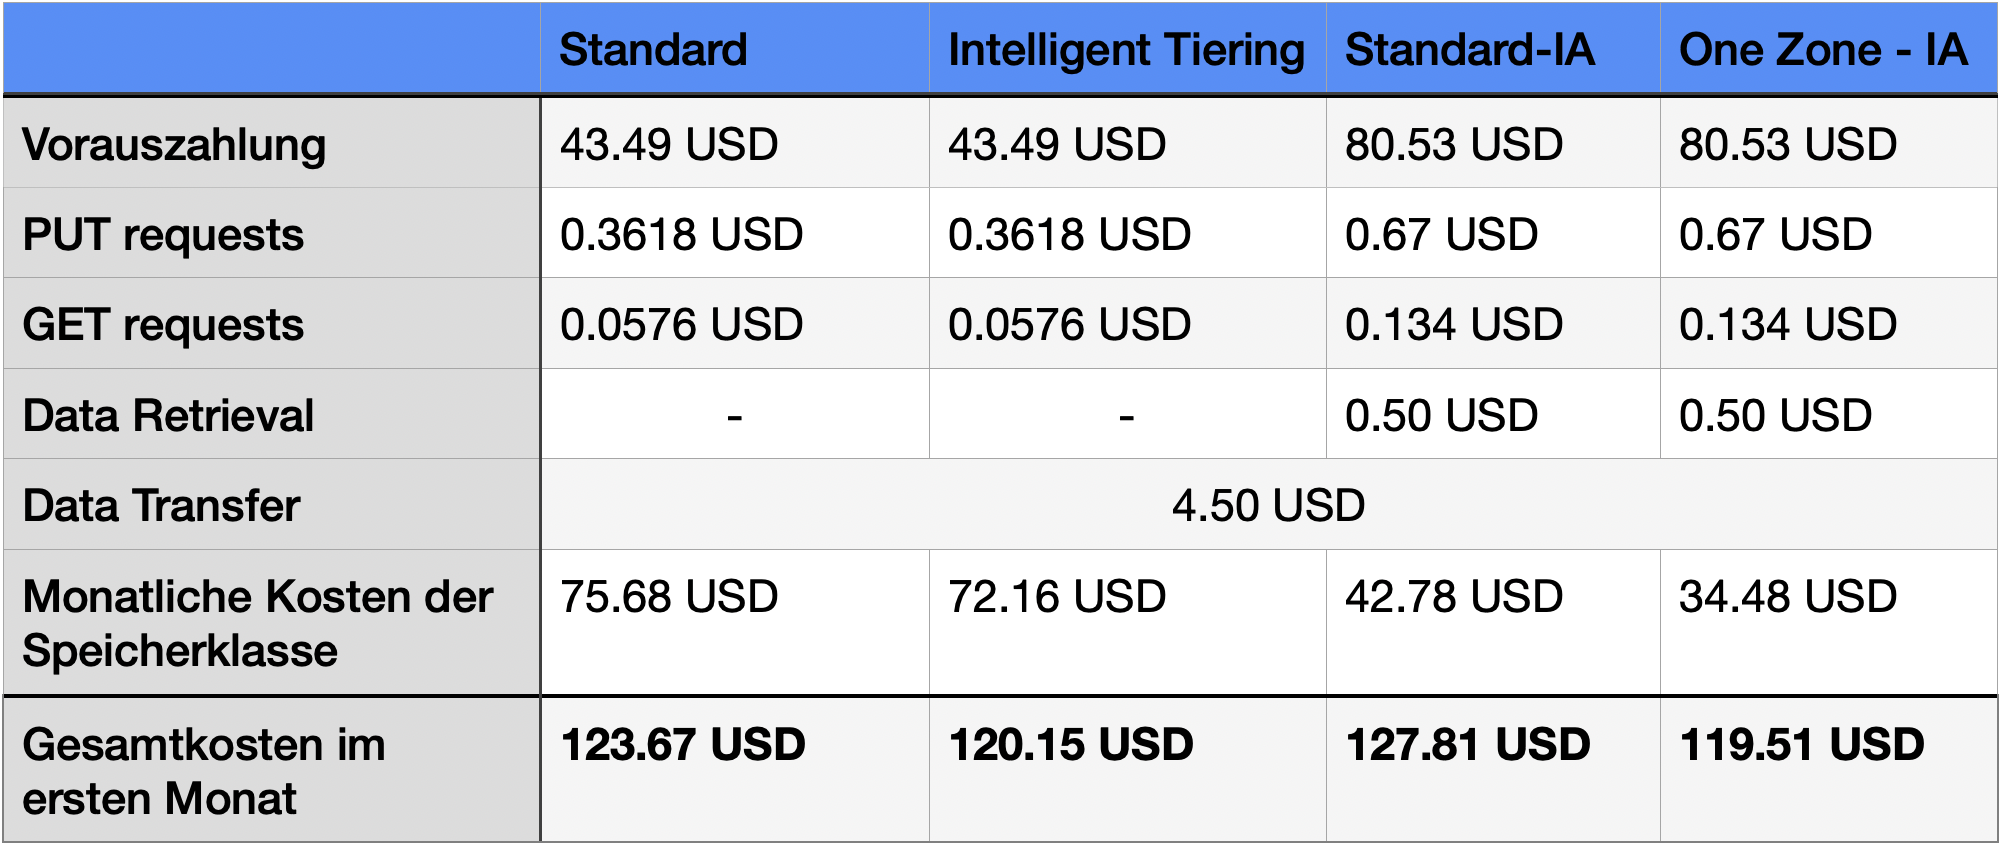
\includegraphics[width=13cm,keepaspectratio]{Pictures/AWSGesamtkosten.png}
	\caption{Zusammenfassung der Gesamtkosten für AWS S3 pro Speicherklasse}
\end{figure}

In dieser Abbildung werden in der letzten Zeile der Tabelle die Gesamtkosten der Speicherklassen pro Monat veranschaulicht. Die Gesamtkosten im ersten Monat der Speicherklasse Standard beträgt 123.67 USD. In diesen Kosten stecken die Vorauszahlungskosten, die PUT und GET Request Gebühren und die Datenübertragungsgebühren. Im Intelligent Tiering und Standard sind die Datenabrufgebühren nicht enthalten, da es dafür keine Gebühren abgezogen werden. Die Gesamtkosten des Intelligent Tiering pro Monat beträgt 120.15 USD. Die Kosten des Intelligent Tiering hängen jedoch von der Speicherverteilung ab. Die Kosten sind grobe Werte und können von der Verteilung des Speichers in verschiedene Speicherklassen in Prozent abhängen. Bei der Standard-IA Speicherklasse sind es mit 127.81 USD Kosten die teuersten Kosten im Vergleich zu den anderen Speicherklassen. Die One Zone-IA ist mit 119.51 USD die billigste Speicherklasse.

\newpage        

In Google Cloud gibt es keine Vorauszahlungen im Vergleich zu AWS. Hier unterscheiden sich die Gesamtkosten der verschiedenen Speicherklassen zu AWS. In der folgenden Abbildung werden die Gesamtkosten zusammengefasst:

\begin{figure}[h]
	\centering
	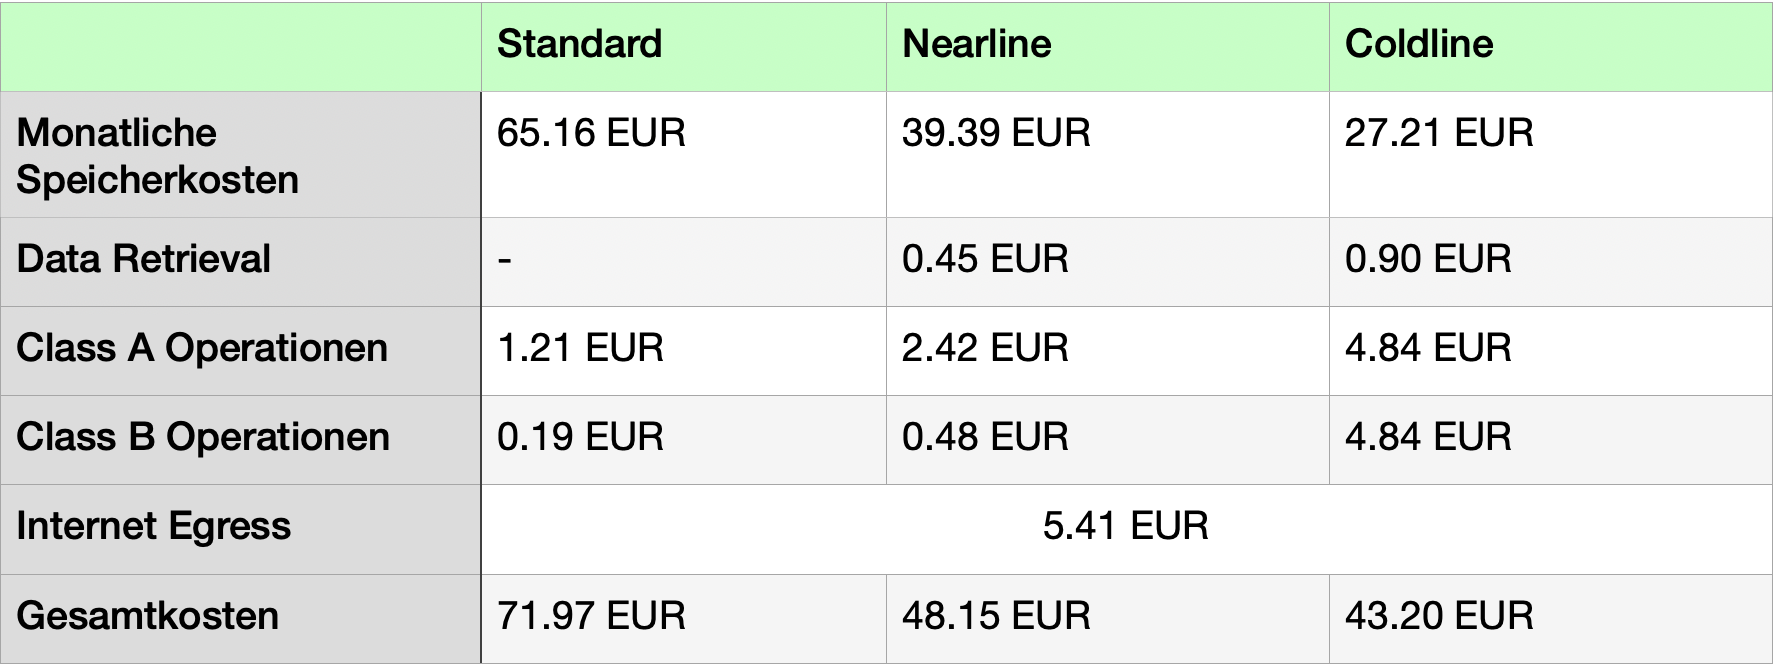
\includegraphics[width=13cm,keepaspectratio]{Pictures/GCgesamtkosten.png}
	\caption{Zusammenfassung der Gesamtkosten für GC Storage pro Speicherklasse}
\end{figure}

Die Gesamtkosten bilden sich hauptsächlich aus den Datenabrufen, Class A und Class B Operationen, was die PUT und GET beinhalten und die Internet Egress, ausgehend von Google Cloud zum Internet, beispielsweise beim Abrufen von Dateien. Wobei keine Gebühren für die Datenabrufe der Standard Speicherklasse anfallen. Die Gesamtkosten des Standards beträgt 69.86 Euro, der Nearline 42.61 Euro und des Coldline 25.36 Euro. 

\newpage
\subsection{Messungsergebnisse}

In diesem Abschnitt werden die Messungsergebnisse der Performance Analyse bereitgestellt. Die Speicherklassen Standard, Standard-IA und One Zone-IA von AWS wurden jeweils mit Standard, Nearline und Coldline von GC verglichen. Im folgenden werden die Ergebnisse der Upload Geschwindigkeit aller Speicherklassen als Liniendiagramm dargestellt:

\begin{figure}[h]
	\centering
	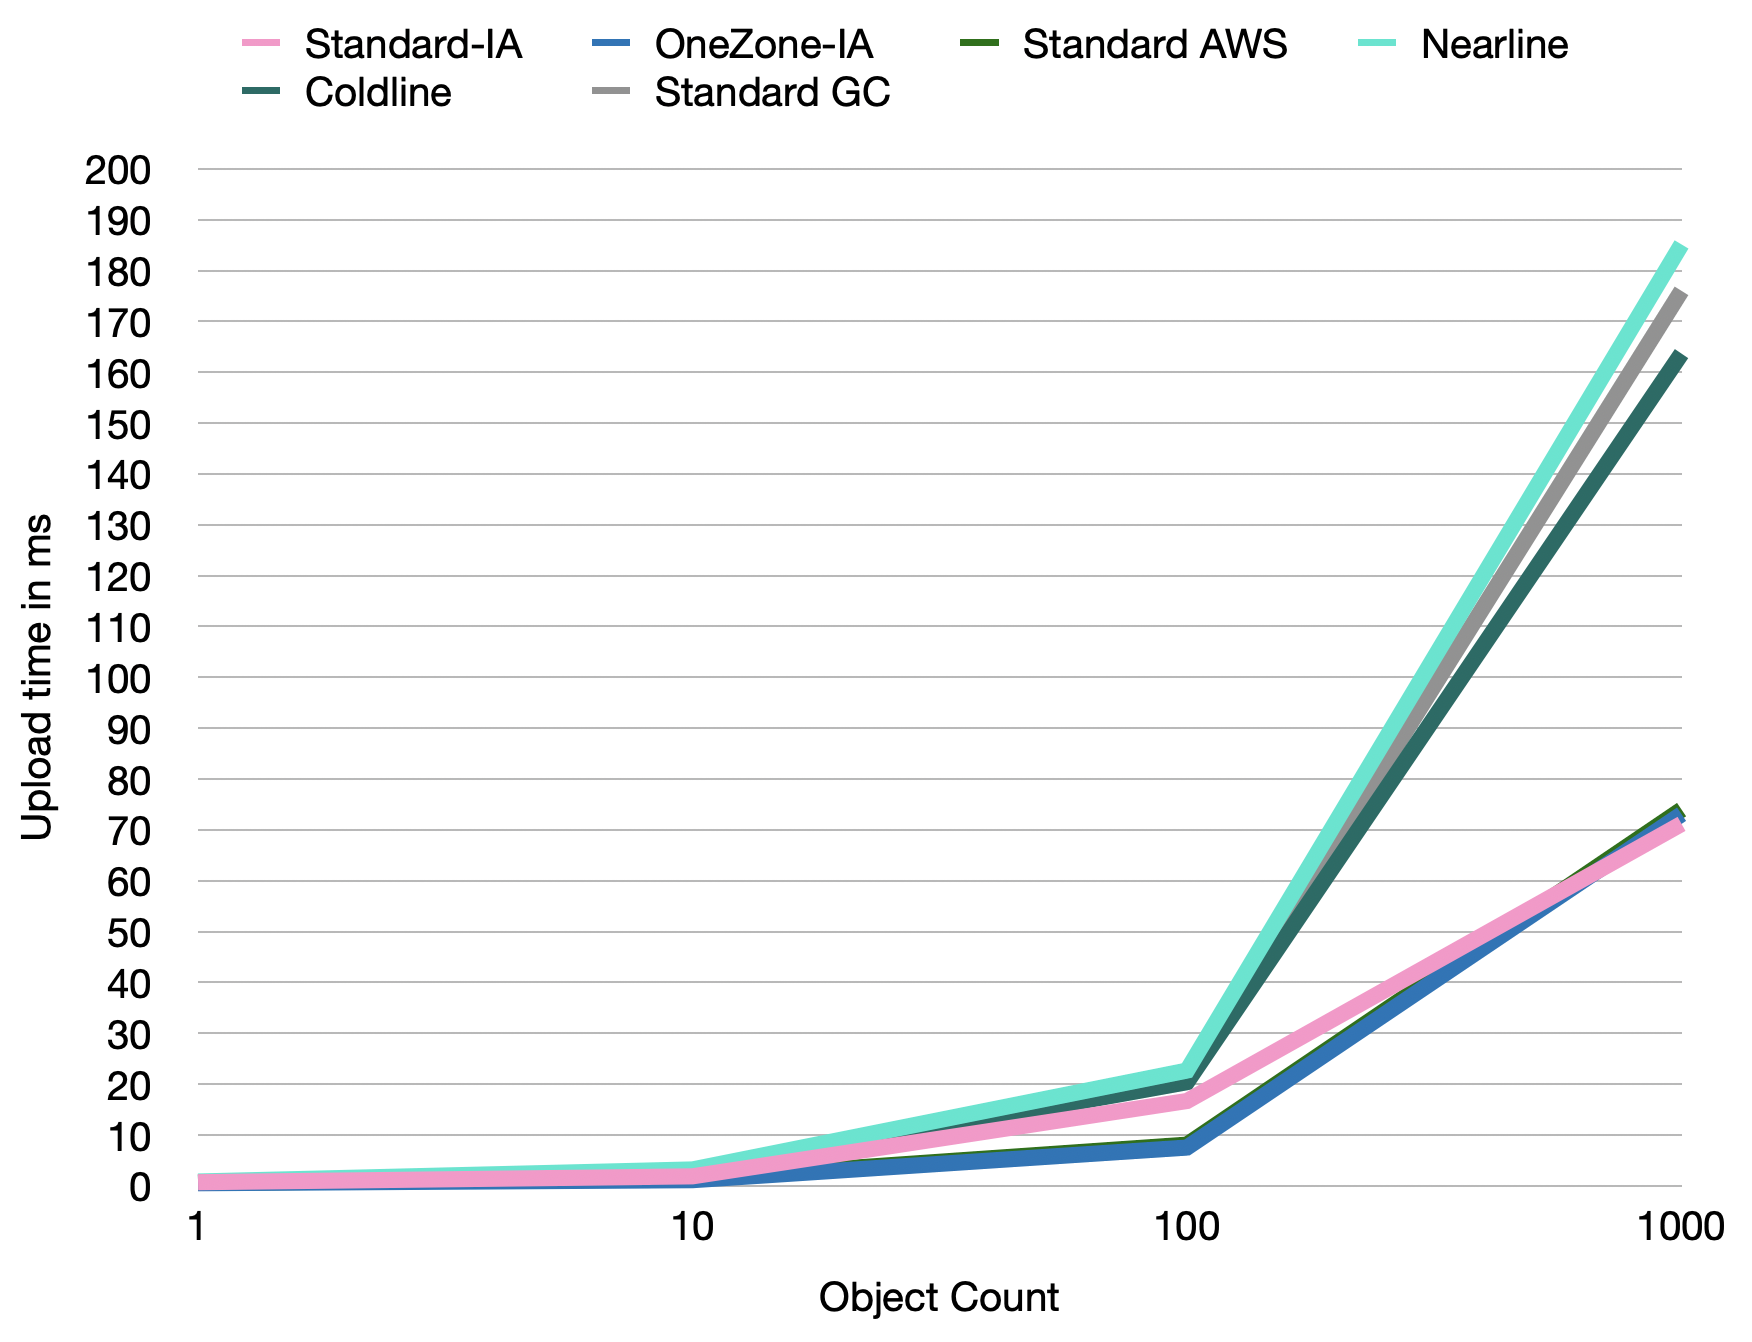
\includegraphics[width=13cm,keepaspectratio]{Pictures/UploadTime.png}
	\caption{Liniendiagramm - Upload Zeit der verschiedenen Speicherklassen}
\end{figure}	

In der obigen Abbildung wird die Upload Geschwindigkeit in Millisekunden auf der Y-Achse beschrieben. Die X-Achse beschreibt die Objektanzahl, die für jede Speicherklasse hochgeladen wurde. Die Farben unterscheiden die verschiedenen Speicherklassen voneinander, wobei die Speicherklassen von AWS jeweils nebeneinander platziert sind, genauso wie für die Speicherklassen von GC. Die genauen Zahlen vom Abschnitt 3.5.1 wurden in diesen Diagramm eingefügt, um die Unterschiede zwischen den Speicherklassen beider Provider zu visualisieren. So liegen die Speicherklassen von AWS im Graph nah beieinander, ähnlich wie mit den Speicherklassen von GC. Beim Hochladen von einer Datei bis hin zu zehn Dateien gibt es minimale Unterschiede und sind sehr nah beieinander. Diese Werte liegen unter 3033 Millisekunden, was ungefähr 3 Sekunden entspricht. Die Linien gehen ab dem Hochladen von 11 bis 1000 Dateien stärker auseinander. Die drei Speicherklassen von GC entfernen sich von den drei Speicherklassen von AWS. Ab 100 Dateien gibt es erneut einen Knick und die Speicherklassen von GC entfernen sich weiter von den AWS Speicherklassen. Die GC Speicherklassen wachsen steiler nach oben als bei AWS und bewegen sich in höheren Millisekunden Bereichen von ungefähr 20 000 Millisekunden bis hin zu 190 000 Millisekunden, umgerechnet bei ungefähr 20 bis 190 Sekunden. AWS bewegt sich dabei maximal bis 140 000 Millisekunden, umgerechnet bis 140 Sekunden. 

\newpage

Bei der Download Geschwindigkeit unterscheiden sich die Werte vom Upload stärker, denn die Zahlen für den Download bewegen sich in Bereichen von 16 bis hin zu 1556 Millisekunden. Hier steigen die Werte nicht höher als 2 Sekunden. In der folgenden Abbildung wird dies veranschaulicht:

\begin{figure}[h]
	\centering
	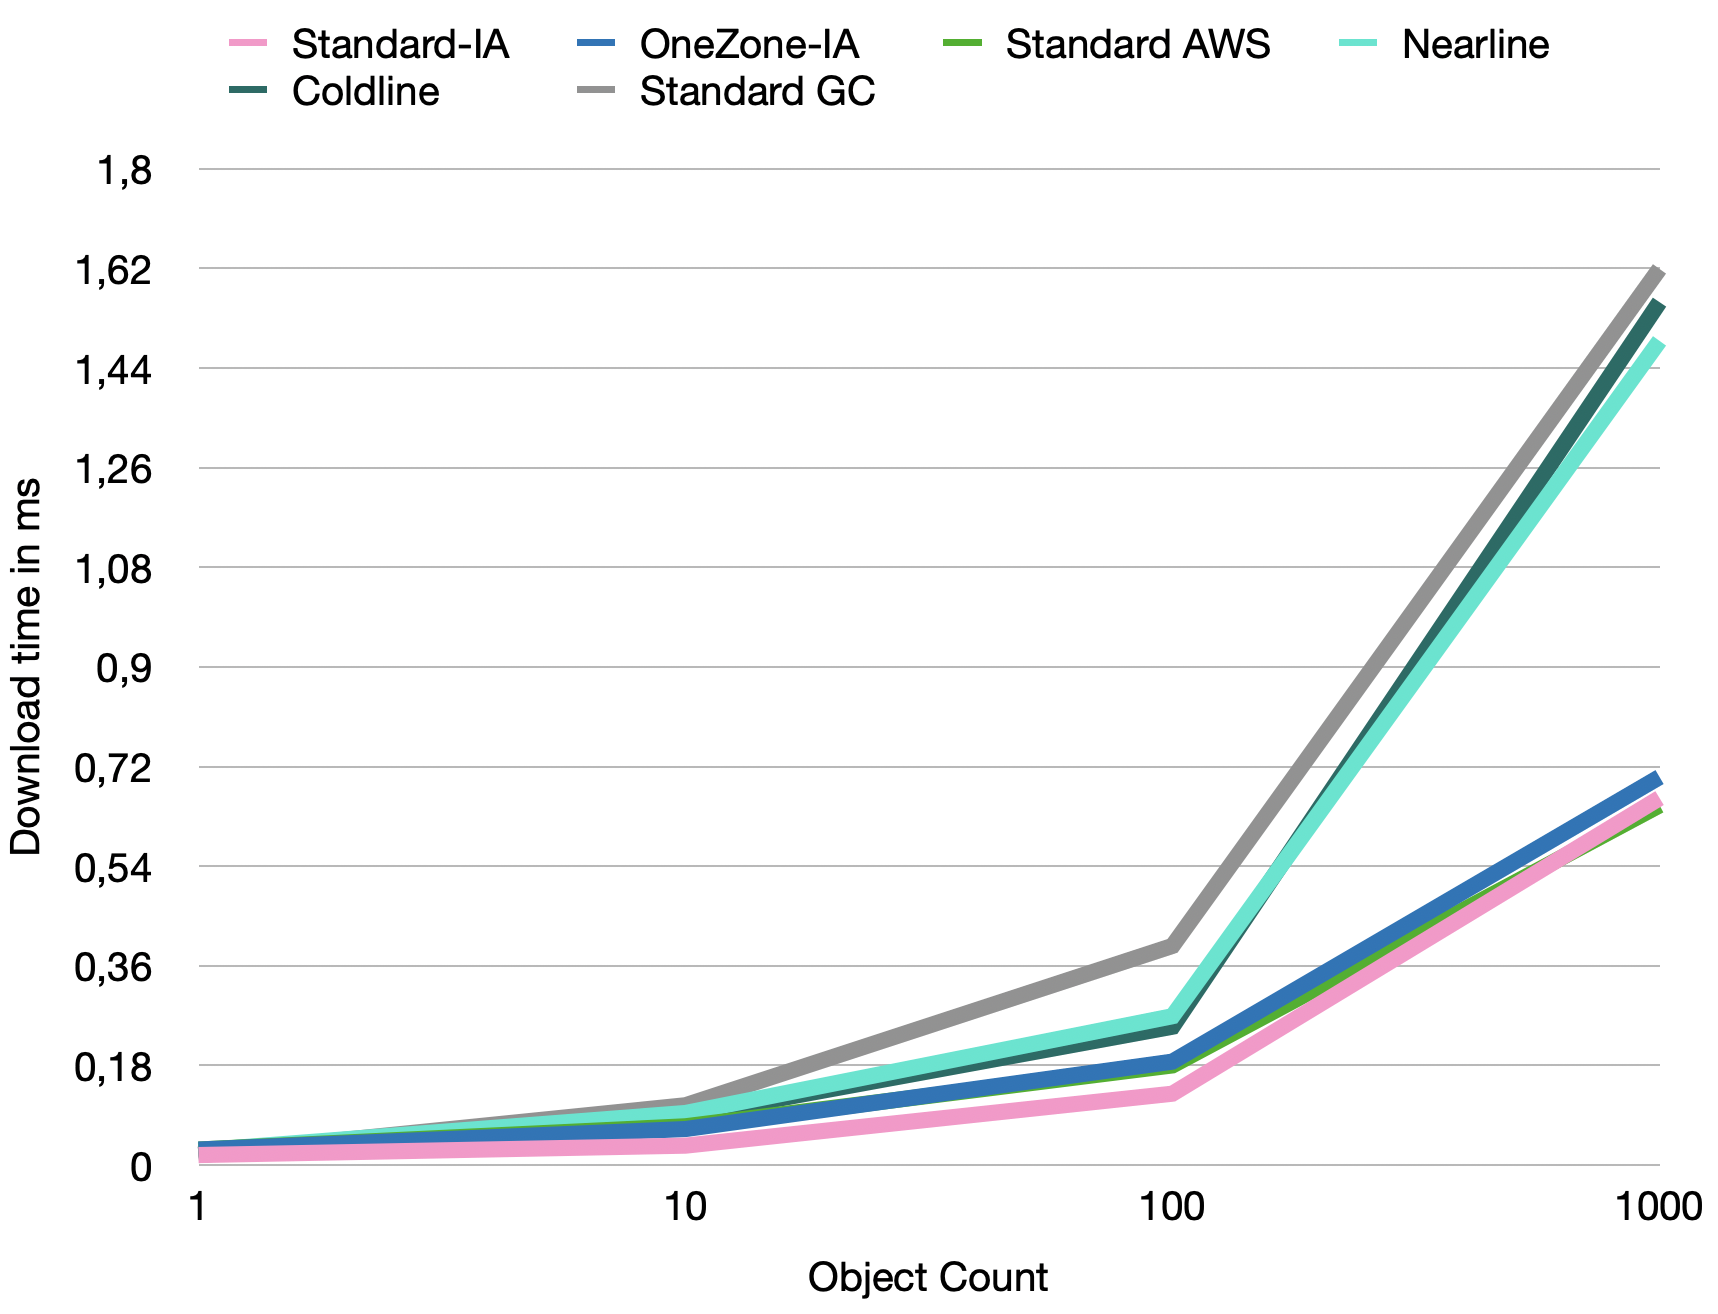
\includegraphics[width=13cm,keepaspectratio]{Pictures/DownloadTime.png}
	\caption{Lininediagramm - Download Zeit der verschiedenen Speicherklassen}
\end{figure}

Dieser Graph ähnelt dem Graph für den Upload in Abbildung 4.2.3. Denn auch hier entfernen sich die Linien für die GC Speicherklassen von den Linien der AWS Speicherklassen. Ab Downloads von zehn Dateien trennen sich die Cloud Provider voneinander. Die Coldline Speicherklasse von GC hat dabei am längsten mit 1556 Millisekunden für den Download von 1000 Dateien gebraucht. Die schnellste Speicherklasse von AWS ist die OneZone-IA mit 569 Millisekunden beim Download von 1000 Dateien. Wobei die Speicherklassen von AWS nah beieinander liegen und weniger als 1 Sekunde für den Download gebraucht haben. Bei GC dauern die Downloads von 1000 Dateien mindestens 1.5 Sekunden. Im Bereich von einer bis zehn Dateien bewegen sich die Speicherklassen in unter 160 Millisekunden Bereichen. Jedoch gibt es bei zehn Dateien bereits erste minimale Unterschiede die langsam wachsen.\\
 
\chapter{Diskussion}

In diesem Kapitel werden die Kalkulations-, und Messergebnisse der Performance analysiert und interpretiert. Anschließend wird der Prototyp bewertet und dabei auf dessen Grenzen eingegangen.
  
\section{Analyse und Interpretation der Ergebnisse}

Basierend auf der Kostenanalyse und den Ergebnissen der Kalkulation ergibt sich, dass die Speicherklassen OneZone-IA von AWS und Coldline von GC die niedrigsten Kosten für die Speicherung von Daten aufweisen. Jedoch sind Datenabrufe in diesen Speicherklassen als kostenintensiv zu betrachten. In der Coldline-Klasse belaufen sich die Kosten für Klasse A-, und B-Operationen jeweils auf 4,84 Euro, während bei AWS PUT-Anfragen, die mit Klasse A gleichzusetzen sind, 2,50 Euro und GET-Anfragen, die mit Klasse B gleichzusetzen sind, 0,50 Euro betragen. Insgesamt sind die Kosten für die Coldline-Klasse im Vergleich zur OneZone-IA-Klasse jedoch günstiger.\\ 

Die Entscheidung für OneZone-IA als Speicherklasse birgt das Risiko auf die Nicht-Verfügbarkeit von Daten bei Ausfall der AZ, da die Daten nur in einer Verfügbarkeitszone gespeichert werden. Dies steht im Widerspruch zu den Anforderungen von leoticket an eine hohe Verfügbarkeit. Obwohl die Speicherkosten in dieser Klasse am niedrigsten sind, sind die Kosten für Datenabrufe im Vergleich zu anderen Speicherklassen höher. Für leoticket ist es jedoch von Bedeutung, auf Objekte mindestens zweimal zugreifen zu können und sie den Kunden zur Verfügung zu stellen. Bei älteren Daten, die mehrere Jahre zurückliegen, kann es ratsam sein, die Objekte in S3 Glacier Instant Retrieval oder in GC Archive Storage zu verschieben, um Kosten für die Archivierung einzusparen und die Daten in Bereichen von Millisekunden zur Verfügung stehen können.\\

Die Verfügbarkeit der Coldline-Klasse ähnelt der OneZone-IA-Klasse. Die Datenabrufe in dieser Klasse können mehrere Stunden dauern. Sie ist nicht für Szenarien geeignet, die einen sofortigen Zugriff auf Daten erfordern oder in denen häufiger auf die Daten zugegriffen werden muss. Im Gegensatz zur OneZone-IA ist die Coldline-Klasse jedoch nicht auf eine einzelne Verfügbarkeitszone beschränkt. Aufgrund ihrer geringeren Kosten und der Verfügbarkeit in mehreren Availability Zones ist Coldline die bessere Option für die langfristige Archivierung von Daten. Da die Kosten für Datenabrufe in dieser Klasse höher sind als in allen anderen Speicherklassen, ist sie nicht geeignet für Daten, auf die mehr als einmal zugegriffen werden muss.\\

Im Rahmen der Performance-Analyse zeigte die OneZone-IA-Klasse eine bessere Leistung als die Coldline-Klasse. Bereits beim Upload von zehn Dateien war die OneZone-IA-Klasse deutlich schneller. In diesem Szenario war sie 20.6\% schneller wie die Coldline-Klasse. Beim Upload von 100 Dateien wurde ein Unterschied von 63\% festgestellt, wobei die Coldline-Klasse etwa 20 Sekunden und die OneZone-IA-Klasse nur etwa sieben Sekunden benötigte. Bei 1000 Dateien bewegten sich beide Speicherklassen im Minutenbereich, wobei auch hier die OneZone-IA-Klasse 55.34\% schneller wie die Coldline-Klasse war. Beim Download von Dateien bewegten sich beide Klassen in Millisekunden Bereichen. Ab 1000 Dateien war die Coldline-Klasse ungefähr 55\% langsamer als die OneZone-IA-Klasse.\\

Die Speicherklassen Standard-IA und Nearline weisen bei den Speicherkosten nur geringfügige Preisunterschiede  auf, die sich auf maximal zwei Euro belaufen. Dabei ist Nearline maximal zwei Euro günstiger als Standard-IA. Die Standard-IA eignet sich für seltene Datenabrufe, die jedoch eine schnellere Zugriffszeit erfordern, wenn sie benötigt werden. Die Nearline-Klasse ähnelt der Standard-IA und ist ebenfalls für Daten gedacht, die gelegentlich im Zeitraum von Wochen oder Monaten abgerufen werden. Sie ist ideal für Datensicherung, Datenmigration und Datenarchivierung. Beide Speicherklassen bieten einen Kompromiss zwischen Kosteneinsparungen und Datenzugriffszeiten.\\

Während der Performance Analyse wurden diese beiden Speicherklassen verglichen, da sie ähnliche Eigenschaften aufweisen. Es stellte sich heraus, dass sich die Dauer des Uploads und Downloads erst ab 10 Dateien zu unterscheiden began. Dabei war die Standard-IA beim Hochladen und Herunterladen der zehn Dateien fast dreimal so schnell wie die Nearline-Klasse. Die Nearline-Klasse schnitt beim Hochladen schlechter ab. Beim Herunterladen von Dateien gab es jedoch nur minimale Unterschiede, wobei die Nearline bei 1000 Dateien 61.55\% langsamer war wie die Standard-IA.\\

Die Standardklassen beider Anbieter weisen kaum Unterschiede bei den PUT- und GET-Anfragen auf. Allerdings sind die Speicherungskosten in der Standardklasse von AWS 9.27\% höher als bei GC. Beide Klassen eignen sich für Daten, auf die häufig zugegriffen wird und die eine hohe Verfügbarkeit, schnelle Zugriffszeiten und geringe Latenzzeiten erfordern. Beide Standardklassen sind für den allgemeinen Gebrauch optimiert, wobei die Speicherungskosten in diesen Klassen im Vergleich zu anderen Speicherklassen am höchsten sind.\\

Bei der Performance-Analyse schnitt die Standardklasse von AWS ab zehn Dateien etwa 54.4\% besser ab als die entsprechende Klasse von GC. Beim Hochladen von 100 Dateien war die AWS-Standardklasse etwa 60.9\% schneller und bei 1000 Dateien etwa 58\% schneller wie die GC Standardklasse. Beim Herunterladen von Dateien waren die Unterschiede nicht groß genug, um eine eindeutige Aussage über die Überlegenheit einer Klasse zu treffen. Allerdings war die AWS-Standardklasse bei 1000 Dateien etwa 60\% schneller.\\

Es ist anzumerken, dass bei den AWS Kosten auch die Vorabzahlung der Speicherung aller Objekte enthalten ist. Bei GC gibt es hingegen keine Vorabzahlung für die Speicherung von Objekten. Aus diesem Grund und auch durch die niedrigeren Gebühren der Speicherung ist GC die kostengünstigere Datenspeicherung.\\

Insgesamt war die Dauer des Uploads und Downloads der Speicherklassen von AWS in der Performance-Analyse niedriger als bei GC. Ab einer Datei traten bereits erste Unterschiede auf, wobei GC mehr Zeit in Anspruch nahm. Die Performance-Messungen basieren jedoch lediglich auf groben Schätzungen innerhalb einer virtuellen Umgebung, die von Hetzner Cloud bereitgestellt wurde. Hier ist anzumerken, dass der Hetzner Server näher am AWS Server liegen und deshalb bessere Ergebnisse in der Performance als GCP erzielen kann. Faktoren wie die Auslastung des Netzwerks können die Ergebnisse beeinflussen und stellen keine aussagekräftigen Performance-Ergebnisse dar.\\

\section{Bewertung des Prototyps}

Für die Bewertung des Prototyps wurden die Anforderungen von leoticket herangezogen. Dabei war es wichtig, den Prototypen so zu bauen, dass die sichere Speicherung gedeckt war. Für die Deckung der sicheren Speicherung wurden verschiedene Methoden betrachtet, die beide Cloud Provider anboten. Dabei implementiert der Prototyp die SSE-KMS Methode beider Provider. Durch die eigene Erstellung des Schlüssels in der KMS von AWS und GC hat der Nutzer mehr Kontrolle, da die Schlüssel von ihm selbst erstellt werden. Der Schlüssel wird vom KMS gespeichert und muss daher nicht vom Nutzer extern gespeichert und verwaltet werden. Der Prototyp kann jedoch so umgebaut werden, dass auch eine andere Methode wie die SSE-C verwendet werden kann. Die SSE-C bietet eine höhere Sicherheit, da der Nutzer den Schüssel selbst generieren und speichern muss. Dies führt aber auch zum Risiko, den Schlüssel zu verlieren. In diesem Fall kann auf die Objekte im Bucket nicht mehr zugegriffen werden. Noch ein Kriterium von leoticket war die hohe Verfügbarkeit der Daten. Der Prototyp wurde so gebaut, dass der Nutzer die Speicherklasse für AWS selbst wählen kann. In GC funktioniert das, indem das Bucket die richtige Speicherklasse bereits eingestellt hat. Für die Verfügbarkeit sind jedoch die Cloud Provider verantwortlich. Hier versprechen beide Provider eine Verfügbarkeit von mindestens 99.5\%. Diese Verfügbarkeit hängt von den verschiedenen Speicherklassen ab. Über Terraform werden Buckets automatisch mit den Einstellungen konform zu den Anforderungen von leoticket erstellt. Diese beinhalten die Konfigurationen von:

\begin{itemize}
	\item Object Versioning
	\item Lifecycle Rules
	\item Object Ownership
	\item Data Encryption
	\item Object Logging
	\item Bucket ACL
	\item Public Access Block
\end{itemize}

Die Objekt Versionierung dient zur Steigerung der Verfügbarkeit, falls Daten unerwünscht gelöscht oder überschrieben werden. Für die Anforderung der Integration in Software-Produkte wie leoticket sorgen die SDKs der beiden Provider. Diese unterstützen verschiedene Programmiersprachen. Sie werden durch Spring Boot unterstützt und können auch mit Maven oder Gradle gebaut werden. Die Anbindung verläuft gemäß der offiziellen Dokumentation der beiden Cloud Provider. Die Dokumentationen sind verständlich und auf dem aktuellsten Stand und beschreiben deren API. AWS und GC bieten auch neue Versionen an und updaten die SDKs. Die Generierung der signierten URLs ist für die Bereitstellung der Dateien zuständig. Diese Anforderung war das Hauptmerkmal von leoticket. Dabei ist es bei beiden Providern möglich, signierte, zeitlich begrenzte URLs zu generieren und diese Nutzern bereitzustellen. Empfänger der URL können so ihre Tickets und Rechnungen herunterladen. Für die Performance Analyse wird eine Methode zur Verfügung gestellt, die Testdateien in der Größe von 100 KB erstellen und in Buckets hoch- und herunterladen kann.\\

Insgesamt ist der Prototyp ausbaufähig und stellt für diese Arbeit einen Vergleich zwischen beiden Cloud Providern dar. Für den besseren Vergleich beider Cloud Provider wurden die Technologien ausprobiert und genutzt. Durch Änderungen an der Terraform Konfiguration, der Speicherklassen Variable für AWS und an der Methode der Datenverschlüsselung kann der Prototyp angepasst werden. Eine Schwäche des Prototyps besteht darin, dass keine genauen Performance Messungen durchgeführt werden können aufgrund genannter Einflüsse, welche die Ergebnisse beeinflussen können. Er dient lediglich dem groben Vergleich. Eine weitere Schwäche des Prototyps besteht darin, dass Entwickler bei der Integration des Prototyps in eigenen Anwendungen Anpassungen durchführen müssen, indem die Hauptklasse des Prototyps so umgebaut werden muss, dass sie dem gewünschten Verhalten entspricht.
\chapter{Fazit}

In diesem Kapitel werden die zuvor gestellten Fragen beantwortet. Darüber hinaus wird die potenzielle Anwendung des Prototyps diskutiert.

\section{Beantwortung der Forschungsfrage}

Folgende Fragen wurden am Anfang gestellt:

\begin{itemize}
	\item Welches Speichersystem ist im Hinblick auf Kosten, Performance und Verfügbarkeit für die Persistenz von Binärdaten besonders geeignet? 
	\item Wie können Daten durch sichere, zeitlich begrenzte URLs bereitgestellt werden?
\end{itemize}

Um die erste Frage zu beantworten, werden die Punkte des theoretischen Teils aufgegriffen. Es wurden verschiedene Speicherarten wie Objekt-, Block-, und File Storage untersucht. Dabei stellte sich heraus, dass Objekt Storage als Speichersystem für die Anforderungen von leoticket geeignet ist. Einige Cloud Provider stellen Objekt Storage zur Speicherung von Daten zur Verfügung und sind im Markt stark vertreten. Es wurden die zwei größten Cloud Provider AWS und GCP betrachtet und eine Vergleichsbasis hergestellt im Hinblick auf Kosten, Performance, Verfügbarkeit, Sicherheit, Bereitstellung der Daten und API Anbindungen. Bei der sicheren Speicherung war es wichtig, dass die Daten vertraulich gespeichert werden und nur Berechtigte Zugriff auf sie haben.\\

 Datenverschlüsselungsmethoden wurden bei beiden Cloud Providern betrachtet und dabei festgestellt, dass die SSE C zwar die stärkste unabhängige Sicherheit bietet, jedoch das Risiko besteht, selbstverwaltete und gespeicherte Schlüssel zu verlieren. Außerdem müssten Mitarbeiter dafür geschult werden, was extra Aufwand bedeutet. Aus diesem Grund wurde für die Implementierung des Prototyps die SSE-KMS customer-managed Methode verwendet, damit der Nutzer die Schlüssel in der KMS von den Providern selbst erstellen und verwalten kann. So bleibt die Kontrolle erhalten und verschafft höhere Sicherheit. Je nach den gewählten Speicherklassen versprechen beide Anbieter eine Verfügbarkeit von mindestens 99.5\%. Bei der Untersuchung der Speicherklassen in Verbindung mit Kosten und Performance stellte sich heraus, dass die Standard-IA von AWS und die Nearline von GC besser zu den Anforderungen von leoticket passen. Da die Latenz für leoticket kein Kriterium darstellt und vernachlässigt werden kann, fallen die Standard Klassen beider Provider weg. Die Standardklassen bieten zwar eine leistungsfähige Speicherlösung, jedoch gehen die eingesetzten Mittel über das hinaus, was tatsächlich benötigt wird. Da Daten über einen Zeitraum von bis zu zehn Jahren gespeichert werden müssen, sind die Speicherkosten für die Standardklassen im Vergleich zu anderen Optionen zu hoch. Die Speicherung der Daten auf längerer Sicht steht mehr im Fokus, da auf eine Datei im Durschnitt nur zweimal zugegriffen wird. Die OneZone-IA fällt ebenfalls weg, da die Daten nur in einer Availability Zone gespeichert werden. Das Risiko ergibt sich durch Nicht-Verfügbarkeit der Daten durch Speicherung in lediglich einer Zone. Daten müssen auf Abruf schnell zugreifbar sein, deshalb sind die OneZone-IA und die Coldline nicht geeignet, da sie eher für selten abgerufen Daten angepasst sind. Die Abrufkosten dieser Speicherklassen sind am höchsten und nicht zu empfehlen.\\

Insgesamt wird für die Persistenz von Binärdaten ein Object Storage mit den Speicherklassen Standard-IA von AWS und Nearline von GC empfohlen. Sie bieten die nötigen Funktionen an, um die Anforderungen zu decken und kostengünstig Daten für längere Zeit zu speichern und dabei eine hohe Verfügbarkeit und Performance zu bieten. Die Entscheidung hängt auch von den persönlichen Präferenzen des Unternehmens ab. Beide Provider bieten eine gute Objektspeicherung kostengünstig und leistungsfähig an.\\

Bei der zweiten gestellten Frage geht es um die Bereitstellung der Daten durch signierte zeitlich begrenzte URLs. Diese Frage wurde durch Vergleichen der SDKs bei der Implementierung des Prototypen untersucht und bewertet. Es stellt sich heraus, dass beide Cloud Provider die Funktionen anbieten, signierte URLs zu erstellen und zeitlich begrenzt bereitzustellen. Mithilfe des Prototypen kann man Dateien hochladen und sie durch URLs bereitstellen. Durch Klicken auf den generierten Link werden die Daten heruntergeladen. So kann verhindert werden, Dateien direkt in Email Anhängen hinzuzufügen, sondern durch Links bereitzustellen. Diese Dateien werden von den Buckets entschlüsselt heruntergeladen und Nutzer können ohne AWS oder GC Credentials darauf zugreifen. Über den Prototypen kann man die Minuten, in denen der Link valide ist, angeben. GC und AWS stellen ausführliche Dokumentationen auf den offiziellen Seiten bereit, um diese Funktionen zu implementieren und in verschiedenen Programmiersprachen anzuwenden.\\

So kann leoticket vom alten System zu der neuen empfohlenen Speicherlösung wechseln, um Daten sicher und schnell bereitzustellen und für längere Zeit zu speichern. Es ist zu beachten, dass diese Arbeit lediglich dem Vergleich und der Veranschaulichung beider Cloud Provider dient und dass jedes Unternehmen unterschiedliche Anforderungen aufweist. Diese Arbeit dient als Stütze und zum Testen der Technologien auf Basis des Prototypen. 

\section{Potenzielle Anwendung des Prototyps}

Der Prototyp wurde entwickelt, um sich mit den Technologien der Cloud Provider auseinanderzusetzen. Durch die Anwendung konnten Performance Analysen durchgeführt werden, die zur Auswahl des Speichersystems beitragen. Die Anwendung kann ausgebaut werden, sodass sie den Bedürfnissen der Unternehmen entspricht. Sie stellt eine Bibliothek dar, die in eigene Anwendungen integriert werden kann. Um sich mit den Technologien vertraut zu machen, können Dateien hoch- und heruntergeladen werden. Außerdem ist es möglich Terraform Buckets mit den benötigten Einstellungen und Rechten zu erstellen ohne die Cloud Konsole verwenden zu müssen.\\

Der Prototyp wurde dabei an die Anforderungen von leoticket angelehnt und angepasst, damit er in das Produkt integriert werden kann. Er dient zur Hilfestellung für das Wechseln von Galera Cluster in ein neues Objekt Storage System für Binärdaten. 

\chapter{Danksagung}



%%%%%%%%%%%%%%%%%%%%%%%%%%%%%%%%%%%%%%%%%%%%%%%%%%%%%%%%%%%%%%%%%%
% Literaturverzeichnis ausgeben
%%%%%%%%%%%%%%%%%%%%%%%%%%%%%%%%%%%%%%%%%%%%%%%%%%%%%%%%%%%%%%%%%%
\chapter{Literaturverzeichnis}
\markboth{Literaturverzeichnis}{Literaturverzeichnis}
\printbibliography[heading=literatur,keyword=literatur]
\clearpage
\printbibliography[heading=pdf,keyword=pdf]
\clearpage
\printbibliography[heading=online,keyword=online]
\clearpage
\phantomsection

% Anhang

\chapter{Anhang}

\section{Repositories}
\subsection{Github Link}

\large{Prototyp Repository:}\\

HTTPS: \url{https://github.com/gmzbae/handson-cloud-storage.git}

\begin{verbatim}SSH: git clone git@github.com:gmzbae/bachelor-thesis-latex.git\end{verbatim}\\				

\large{Thesis Repository:}\\

HTTPS: \url{https://github.com/gmzbae/bachelor-thesis-latex.git}

\begin{verbatim}SSH: git clone git@github.com:gmzbae/bachelor-thesis-latex.git \end{verbatim}\\

\subsection{Dokumentation}

Code Dokumentation\\
Entwickler Handbuch

\subsection{Code Snippets}

\clearpage

\end{document}






